\documentclass[12pt,a4paper, twoside,]{report}
\usepackage[utf8]{inputenc}
\usepackage{graphicx}
\graphicspath{{graphics/}}

% language
\usepackage[english]{babel}

% color setting
\usepackage[dvipsnames]{xcolor}
\definecolor{halfgray}{gray}{0.55}
%\pagecolor{Gray}
%% dvipsnames color palette: https://www.overleaf.com/learn/latex/Using_colours_in_LaTeX

% cross reference :)
\usepackage{hyperref}
\hypersetup{
    colorlinks=true,
    linkcolor=MidnightBlue,
    citecolor=Periwinkle,      
    urlcolor=BlueViolet,
}
% footnote colour
\renewcommand\thefootnote{\textcolor{RoyalPurple}{\arabic{footnote}}}

% The following sets margins 
\usepackage[a4paper,left=2.5cm, right=2.5cm,top=2.5cm,bottom=2.5cm]{geometry}

% Set line spacing between paragraphs and no indentation
\usepackage[parfill]{parskip}
\setlength{\parskip}{0.3cm} 
% line space
\usepackage{setspace}
\linespread{1.3}
% page layout
\usepackage{fancyhdr}
\pagestyle{fancy}
\fancyhead{}
\fancyhead[RE,LO]{\rightmark}
\fancyhead[RO,LE]{\thepage}
\renewcommand{\headrulewidth}{0pt}
\fancyfoot{}
\fancyfoot[RE,LO]{\thepage}
\fancyfoot[RO,LE]{\leftmark}

% font
\usepackage{times}


% title spacing
\usepackage[newparttoc]{titlesec}

% parts
\titleclass{\part}{top}
\titleformat{\part}[display]
  {\huge\bfseries\centering}{\vspace{5cm}\color{CadetBlue}\partname~\thepart}{0pt}{}
\titlespacing*{\part}{0pt}{40pt}{40pt}

%chapters
\titleformat{\chapter}[display]{\huge}{\color{CadetBlue}\raggedleft{Chapter \thechapter}}{10pt}{\titlerule}


% abstract format
\makeatletter
\renewenvironment{abstract}{%
    \if@twocolumn
      \section*{\abstractname}%
    \else %% <- here I've removed \small
      \begin{center}%
        {\bfseries \huge\abstractname\vspace{\z@}}%  
      \end{center}%
      \quotation
    \fi}
    {\if@twocolumn\else\endquotation\fi}
\makeatother

% table of content format
\usepackage{titletoc}
%part
\titlecontents{part}% <section-type>
  [0pt]% <left>
  {\addvspace{0.5cm}\large\bfseries}% <above-code>
  {\thecontentslabel\quad}% <numbered-entry-format>
  {}% <numberless-entry-format>
  {\hfill\contentspage}% <filler-page-format>

%chapter
\titlecontents{chapter}% <section-type>
  [0pt]% <left>
  {\bfseries}% <above-code>
  {\chaptername\ \thecontentslabel:\quad}% <numbered-entry-format>
  {}% <numberless-entry-format>
  {\hfill\contentspage}% <filler-page-format>
 
 %section
\titlecontents{section}
[5em]
{}
{\contentslabel{3.2em}}
{}
{\titlerule*[1pc]{.}\contentspage}% 
% subsection
\titlecontents{subsection}
[7em]
{} 
{\contentslabel{3.2em}}
{}
{\titlerule*[0.5pc]{.}\contentspage}% 

% glossary
% long-name-desc-loc style
\usepackage[stylemods=longextra]{glossaries-extra}
\setglossarystyle{long-name-desc-loc}
\setglossarypreamble{This list contains the most relevant versions of definitions to this research project}
\makeglossaries
\newglossaryentry{gle}
{
        name=GLE,
        description={(Genomic Location Effect) \\ the influence of a nucleotide's location on the tendency for it to mutate}
}

\newglossaryentry{nucleotide}
{
        name=nucleotide,
        description={same as base; a component of the DNA sequence, \textit{e.g.} A for adenine}
}

\newglossaryentry{base}
{
        name=base,
        description={same as nucleotide; a component of the DNA sequence, \textit{e.g.} A for adenine}
}

\newglossaryentry{sce}
{
        name=SCE,
        description={(Sequence Context Effect) \\ the influence of the flanking bases on a nucleotide's location on the tendency for it to mutate}
}

\newglossaryentry{or}
{
        name=$OR$,
        description={(Odds ratio) \\ a statistic that measures the degree bias for two characteristics to occur. In my case, I measured how mutations favour closed over open chromatin regions}
}

\newglossaryentry{glm}
{
        name=GLM,
        description={(Generalised Linear Model) \\ A class of model that allows the errors (residuals) to follow a different distribution than the normal distribution. The ordinary linear model is one example of this class}
}

\newglossaryentry{pcawg}
{
        name=PCAWG,
        description={(Pan-cancer analysis of whole genome) \\ an international project that sequenced samples of different cancer types. Part of the project also identified somatic mutations and passenger mutations.}
}

\newglossaryentry{icgc}
{
        name=ICGC,
        description={(International Cancer Genome Consortium) \\ an organisation that contributes to the PCAWG project. Access to the mutation file (\textit{i.e.} non US data) from ICGC is not restricted}
}

\newglossaryentry{tcga}
{
        name=TCGA,
        description={(The Cancer Genome Atlas) \\ another contributor to the PCAWG project. Access to the mutation file (\textit{i.e.} US data) from TCGA is restricted}
}

\newglossaryentry{encode}
{
        name=ENCODE,
        description={(Encyclopedia of DNA Elements) \\ a project that studies various genetics and epigenetics data}
}

\newglossaryentry{dhs}
{
        name=DHS,
        description={(DNase Hypersensitivity) \\ a measure of chromatin status - how accessible a genomic region is. Applying the threshold to dnase accessibility helps identify open vs closed genomic regions. This project used data from ENCODE for DHS, where open and closed chromatin regions of the genome have been identified}
}

\newglossaryentry{chromatin}
{
        name=chromatin,
        description={a complex of DNA with histone protein. A genomic region with a very dense complex is not easily accessible to factors like transcription and DNA repair. Such a region is called closed chromatin region, vice versa for open chromatin regions}
}

\newglossaryentry{null}
{
        name=$H_o$,
        description={(Null hypothesis) \\ The null hypothesis assumes a certain characteristic is the same between 2 or more different classes}
}

\newglossaryentry{alternative}
{
        name=$H_a$,
        description={(Alternative hypothesis) \\ The alternative hypothesis assumes a certain characteristic is different between 2 or more different given classes.}
}

\newglossaryentry{f1}
{
        name=$F_1$,
        description={(F1-Score) \\ A measure of accuracy that takes into account both the sensitivity and specificity of the classifier}
}

\newglossaryentry{sensitivity}
{
        name=sensitivity,
        description={a measure of accuracy for how well a classifier can identify certain classes. The sensitivity for a class is the ratio between the number of observations correctly identified and the total number of observations available for that class}
}

\newglossaryentry{specificity}
{
        name=specificity,
        description={a measure of accuracy for how well a classifier can exclude the possibility of other classes when identifying certain classes. The specificity for a class is the ratio between the number of observations correctly identified as that class and the total number of observations identified as that class}
}

\newglossaryentry{confusion matrix}
{
        name=confusion matrix,
        plural=confusion matrices,
        description={a way to report accuracy of a classifier. In this case the row labels are the true classes and the column labels are the predicted classes. The more data points on the diagonals, the higher the accuracy}
}

\newglossaryentry{ml}
{
        name=ML,
        description={(Machine Learning) \\ the process of building a model to learn the patterns of data}
}

\newglossaryentry{model}
{
        name=model,
        description={all the statistical assumptions about the properties and patterns of data}
}

\newglossaryentry{classifier}
{
        name=classifier,
        description={a model that predict categorical data. In other words, the responses of the model are categorical, not numeric}
}

\newglossaryentry{kde}
{
        name=KDE,
        description={(Kernel Density Estimation) \\ the use of a kernel function to estimate the density of a particular data point}
}

\newglossaryentry{kernel function}
{
        name=kernel function,
        description={any function that belongs to a class of continuous and symmetric functions commonly used in density estimation and computation of ``similarity'' between 2 vectors. When applied on every pair of vectors to obtain a kernel matrix, this matrix is positive semi-definite.}
}

\newglossaryentry{positive semi-definite}
{
        name = positive definite,
        description={a matrix $M$ is positive definite if for every element vector $z$, $zMz^\intercal > 0$. In other words, the eigenvalues of $M$ are positive. Additionally, $M$ is positive semi-definite if its eigenvalues are non-negative}
}

\newglossaryentry{density}
{
        name=density,
        description={the density measures the likelihood of finding data $f(x)$ at a particular location $x$. The density throughout the domain of the data is restricted to be 1}
}

\newglossaryentry{intensity}
{
        name=intensity,
        description={the intensity of a data point is the product of its density and the sample size of the data. Accordingly, while ``inheriting'' some characteristics of the density, the intensity throughout the domain of the data is not restricted to be 1}
}

\newglossaryentry{knn}
{
        name=KNN,
        description={($k$-nearest neighbours) \\ a machine learning algorithm that predicts the labels of a data point based on the information from the closest data points to it. The number of closest data points $k$ is a hyper-parameter to be pre-defined. The choice of the distance measures used to identify the closest data points usually depend on the nature of the data}
}

\newglossaryentry{svm}
{
        name=SVM,
        description={(Support Vector Machines) \\ a machine learning algorithm that predicts the labels of a data point based on finding the boundaries between different classes based on the data points near the border of each class. Those data points are also called the support vectors}
}

\newglossaryentry{pval}
{
        name=$p$-value,
        description={the probability for an event to occur assuming the null hypothesis $H_o$ is true. The smaller the $p$, the more evidence we have to reject the null hypothesis}
}

\newglossaryentry{jackknife}
{
        name=jackknife,
        description={a statistical re-sampling technique which is generally used to estimate the variance in a particular statistic of a data sample. This technique re-computes the statistic of interest upon removing one data point from the given sample. The departure of the re-computed statistic from the original statistic indicates how extreme and influential the removed data point is. Repeating the procedure for every data point outputs a collection of re-computed statistics, which represents the estimated range for that statistic}
}

\newglossaryentry{bootstrap}
{
        name=bootstrap,
        description={a statistical re-sampling technique that reconstructs the original data set by randomly drawing data points from that original data set. The idea is that the reconstructed data set should inherit the properties of the original set, and the departure arises mainly from random noise. Similar to the jackknife, the bootstrap can be used to estimate data variance. However, in this project, the bootstrap was used for hypothesis testing}
}

\newglossaryentry{kmer}
{
        name=$k$-mer,
        description={a $k$ base long DNA sequence unit. For example, ACC and GAT are 3-mers while GCTAC is a 5-mer}
}

\newglossaryentry{re}
{
        name=$RE$,
        description={Relative Entropy \\
        a statistic that measures the amount of information available. Generally, information essentially implies variation. Here $RE$ is derived from a GLM.}
}

\newglossaryentry{sommut}
{
        name=somatic mutation,
        description={a mutation that arises in a somatic (non-germline) cell. This mutation can be passed on to the daughter cells of that somatic cell, but not to the offspring of the person that has the mutation}
}

\newglossaryentry{germline_mut}
{
        name=germline mutation,
        description={a mutation that arises in a germline cell. This mutation might be passed on to the offspring of the person that has the mutation.}
}

\newglossaryentry{point_mut}
{
        name=point mutation,
        description={a mutation where there is one single base change to another base}
}


% These Commands create the label style for tables, figures and equations.
\usepackage[labelfont={small,bf}, textfont=small]{caption}
\captionsetup{labelformat=simple, labelsep=period}
\newcommand\num{\addtocounter{equation}{1}\tag{\theequation}}
\renewcommand{\theequation}{\arabic{equation}}



% reference
\usepackage{natbib}



% maths symbols 
\usepackage{amssymb}
\usepackage{amsmath}
\usepackage[cal=pxtx]{mathalfa}


%%%%%%%%%%%%%%%%%%%%%%%%%%%%%%%%%%%%%%%%%%%%%%%%%%%%%%%%%%%%%%%%%%%%%%%%%%%%%%%%%%%%%%%%%%%%%%%%%%%%



\pagenumbering{roman}

\begin{document}
\begin{titlepage}
    \begin{center}
        \vspace*{1cm}
        \Huge
        \textbf{Statistical techniques for studying \\ cancer mutagenesis} \\

        \LARGE
        \vspace{3cm}
            
        \textbf{Anh Phuong Le} \\
        \vspace{1cm}
        \normalsize
        Supervised by Professor Gavin Huttley and Dr Cheng Soon Ong
            
        \vfill
        
        \normalsize    
        A thesis presented for the degree of\\
        Bachelor of Philosophy (Honours) \\
        Word Counts
            
        \vspace{0.8cm}
            
        
\includegraphics[width=0.4\textwidth]{graphics/ANU_Primary_Horizontal_GoldBlack.jpg}
            
        \Large
        Research School of Biology\\
        The Australian National University\\
        Date
            
    \end{center}
\end{titlepage}
\thispagestyle{empty}
% \vspace*{5cm}

\textit{N.B.} Terms in blue can be found in the \hyperref[glossary]{Glossary}. All coloured texts (blue or light purple) are hyperlinked. If you are reading on a computer or an iPad, you can click on the coloured texts to jump to the definitions, the referenced sections or the cited papers.

\vfill
\normalsize
\LaTeX\ template by 
Phuong Le, inspired by André Miede's \href{https://bitbucket.org/amiede/classicthesis/wiki/Home}{\textit{A Classic Thesis Style}} \\
Phuong Le \textcopyright\ October, 2021 \\
Supervisors: Gavin Huttley, Cheng Soon Ong

\newpage
\thispagestyle{empty}

\vspace*{3cm}

\begin{center}
All models are wrong, but some are useful \\ \medskip
--- George Box, statistician ---   

When you give something to someone else, make it pretty \\ \medskip
--- Prof. Michael Martin, ANU ---   

\end{center}

\vspace{2cm}

Through the journey of Honours, I was lucky enough to receive help and advice from many people. I also found that ideas are often generated and refined when they are shared. I understand more what it means by ``If you want to go far, go together''. With that, I would like to share this \LaTeX\ thesis template, which took me quite some time to make, with anyone who wanted it (contact me for the code). It was inspired by André Miede's \href{https://bitbucket.org/amiede/classicthesis/wiki/Home}{\textit{A Classic Thesis Style}}, the code is less fancy but a bit easier for beginners to tweak.

\chapter*{Declaration}
\addcontentsline{toc}{chapter}{Declaration and Impact statement}





This thesis is an account of research undertaken between February 2021 and  October 2021 at Research School of Biology, Joint College of Sciences, The Australian National University, Canberra, Australia.

Except where acknowledged, the material presented in this thesis is, to the best of my knowledge, original and has not been submitted in whole or part for a degree in any university.

\vspace{20mm}  % vertical space

\large
\begin{flushright}
Phuong Le \\
\today
\end{flushright}

\normalsize
\chapter*{Acknowledgements}
\addcontentsline{toc}{chapter}{Acknowledgements}

First, I would like to thank my supervisor Gavin Huttley. Gavin started mentoring me two years ago when I took his course, Bioinformatics, with hardly any programming background. I then did a short project with him the following semester. Finally, I came back to undertake Honours with him this year. Over such a long period of time, my view remains the same, that I am privileged to be his student. He is one of the rare true bioinformaticians who have a profound understanding of all three domains: biology, computing and statistics. He genuinely cares about students' development, not just the outcome of our work. I always feel extremely assured when I talk with him, when he tells me to ``do good science'' and to ``do what we believe is right'' and that he has ``complete confidence in me''. His lab is a family where Katherine is apparently the bad twin and I am the evil twin. I cannot express how grateful I am for being instructed by Gavin. I hope my thesis and everything I do later on in life will make him proud.

Second, I would like to thank my co-supervisor, Cheng-Soon Ong. I have a tremendous respect for his expertise in machine learning and his superpower of communicating with biologists. While being a busy director of a machine learning platform at CSIRO, Cheng always makes time for me whenever I ping him on Slack. He is always concerned that I might be too stressed and that I do not take enough break. He connects me with his brilliant students and employees at Data61 so that I have even more people to hassle. Besides being a teacher, he gives plenty of great career and life advice. I wish I could quote everything he says, but let me just quote one: ``Be kind''.

I would also like to thank the three powerful individuals who control my fate, Aude Fahrer, Eric Stone and Sasha Mikheyev. I would like to acknowledge Eric, whose statistical mindset I find particularly eye-opening. With his experience, Eric's comments and advice have always been spot on. He has also referred me to his employees at the BDSI, whose expertise was in line with what I was doing. I cannot ask for a more helpful examiner. In addition, I would like to thank Aude, who I knew from her first year cancer lectures and her immunology course. Her input on the biological motivation for my project was invaluable. Communicating with her gives me the perfect chance to practice intellectual conversations with people outside my area.

Throughout the project, I had the opportunity to receive technical support from so many people. I wanted to thank anh\footnote{anh: Vietnamese for big brother} Mai Huy Hoang for patiently helping me with the ``computer stuff'' ever since we were high school students until now when he's finishing his degree at the prestigious Peking University. I wanted to thank my ge\footnote{ge: Chinese for big brother} Zixian Cai for his advice on everything, because conveniently for me, he is both a brilliant computer scientist and a senior international student of the same degree. I was also lucky to get help from Cheng's PhD student, Mengyan Zhang, who understands how to implement machine learning algorithms very well. She is kind enough to volunteer to give me advice that always points out both the strengths and weaknesses of my crazy ideas... I wanted to thank anh Hoang Danh Tai at the BDSI for sharing his machine learning experience and James Nichols for discussing Wasserstein distance with me. I wanted to thank Aaron Chuah at the JCSMR for sharing his wide knowledge of genomic databases. 

Thank you to the lovely people, besides my supervisors, who patiently tolerated my incredibly low speed of writing, read and edited different parts of my thesis, they are Soraya Zwahlen, Hanh Vo, Russell Tsuchida, Aaron Chuah, Andrea Do and Tai Hoang. Everyone was from a different background but all of them were so constructive with their feedback. I cannot imagine how much time and effort they have put in proofreading this, especially Soraya, whose comments were super detailed, super harsh but super encouraging at the same time. 

In terms of financial support, I would like to thank the ANU for awarding me the annual Terrell International Undergraduate Scholarships. On top of that, I would like to thank my past employers for letting me work for them to partly support myself when I moved to Australia, they are Susan Howitt, Mark Ellison, Quynh Nguyen, Johannes Zoller, Thuan Truong and Sao Berger. Susan Howitt, in particular, was another mentor of mine. She taught me during her genetics course, gave me honest advice in terms of career development and course selection. She was my referee when I transferred into the PhB. This year, I worked for her as a demonstrator and I can say that she was extremely caring as an employer. 

This year was ridiculously intense for me in many ways on top of the lockdown and I thank friends who were by my side to help me through it. Thank you to Katherine Caley, my lab mate. Throughout the year, Kath knows virtually everything I go through, she is there for me and she helps as much as she can. She enjoys our complaint sessions, she exchanges code with me and co-authors a few of my emails. Thanks to my roommate Chelsea Crew and landlords Brett and Barbara Still for their amazing kindness. Thanks to em\footnote{Vietnamese for little sister/brother} Han Do and Randolph Leong for being great friends and exchanging food with me. Thanks to my old roommate Hanh Vo for supporting me with useful materials even though she is now based in Tasmania (too bad you couldn't be my source of distraction as I was for you last year). Thanks to em Misa Le for being a great friend/roommate and for being the lucky charm who fixed the dodgy wifi just before my final seminar presentation, helped me decide the colour scheme for my thesis and graphics, forced me to enjoy my birthday just a week before thesis submission and pressed the submit button for me. Thanks to my aunt Le Kim Thuy, who has constant fear that I will starve myself to death and sends me heaps of delicious food. Thanks to my best friend Nguyen Thi Ha Anh, who always supports my superstition by being professionally supersitious herself. Thanks to Soraya Zwahlen, Hang Dang, Minh Bui, Thinh Ngo, Emily Tan, Sharwel Lei. And Maksim Lisau.

Another important person who got me through Honours was Spencer Whitney, who convened my Honours cohort. He is extremely experienced with students and he is always ready to help. He has a questionable sense of humour - he likes jokes that target my supervisor Gavin Huttley. I do too. 

Last but not least, I wanted to thank my family back in Vietnam, my mum Nguyen Thanh Thu, my dad Le Minh Quang and my sister Le Khanh Huong. My parents have been supporting me unconditionally. They are my main financial support, without which my study at ANU would have never been possible. But most importantly, they are my biggest emotional support that I can always rely on. When I am tired, I think of home. I guess there is no need to say anything further. 

\newpage
\thispagestyle{plain}
\begin{abstract}
  \addcontentsline{toc}{chapter}{Abstract}
  
\end{abstract}
\newpage

{
  \hypersetup{linkcolor=CadetBlue}
  \tableofcontents
}
\newpage
\label{glossary}
\printglossary
\newpage

\pagenumbering{arabic}

\chapter{Introduction}\label{intro}

Genetically, the process of \gls{carcinogenesis} is operated and characterised by mutations \citep{Stratton2009}. In turn, whether a mutation occurs is determined by whether mutagens can form a \gls{lesion} in the DNA and whether the repair systems can correctly fix the lesion \citep{Chatterjee2017MechanismsMutagenesis}. While every cancer has a different set of mutations, certain mutation patterns have been found exclusive to several cancer types \citep{Alexandrov2013,Polak2015,Campbell2020}. Since all cancers originate from a normal cell \citep{Hanahan2011HallmarksGeneration}, the patterns of cancer \gls{mutagenesis} likely, to some extent, reflect the mutation tendency in the original cell type. During its development, the phenotype of a cancer sample could diverge from that of the original cell, but virtually all mutations prior to the divergence remain in the cancer genome (Figure \ref{fig:drivers_demo}). These divergence events can be caused by driver mutations, \textit{i.e.} mutations that promote cancer cell proliferation \citep{Pon2015}. An average cancer sample consists of only about 4-5 drivers, the rest are passenger mutations, which have neutral effects on the cancer progress \citep{Campbell2020}. Together, the whole history of mutations in a cancer sample helps characterise its mutation profile. 

\begin{figure}[h!]
    \centering
    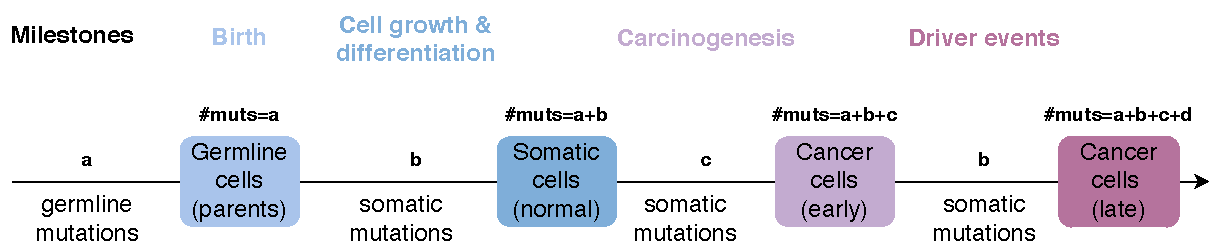
\includegraphics[scale=0.78]{graphics/drivers_demo.pdf}
    \caption{\textbf{Timeline of a carcinogenesis process.} Mutations are generally retained in the genome after each stage of carcinogenesis, even though carcinogenesis and driver events could change the phenotype of the cells. Together, all mutations available in a cancer cell make up it mutation profile. For the purpose of this project, only somatic mutations are considered because germline mutations occur prior to birth and are not the product of the environment of the differentiated cells in which cancer develop.}
    \label{fig:drivers_demo}
\end{figure}


The mutation profile reflects the mechanism of mutagenesis, which offers a great opportunity to study cancer. This project seeks to analyse the invaluable information extracted from the cancer mutation profile, with a hope that our enhanced understanding could potentially help guiding treatment. Furthermore, I seek to exploit this information to predict cancer types by training a \gls{classifier} that only relies on genomic sequencing data. In the long term, such a classifier could be an additional diagnostic tool to existing clinical approaches such as cytology or biopsy \citep{Stone1995Biopsy:Pitfalls}. In this era of next generation sequencing, liquid biopsies are gaining interest as a powerful non-invasive method for early cancer diagnosis because they involve screening for circulating tumour DNA in the blood rather than obtaining samples from a suspected local tissue \citep{Chen2019Next-generationDetection}. Developing a genome-based classifier model means that liquid biopsies could inform not only whether a cancer is present, but also where and what cancer is occurring at an early stage.  

Regarding the scope of the project, two aspects of of a cancer mutation profile were studied: where mutations tend to be found in the genome (hereafter the Genomic Location Effect, GLE) and what \gls{base} changes tend to be found in which genomic sequence context (hereafter the Sequence Context Effect, SCE). Secondly, the project is limited to point mutations, which are the most abundant type of mutations in cancer \citep{Alexandrov2020}. Thirdly, due to the different mutation rates between drivers and passengers, they should be considered separately - I focused on passenger mutations \citep{McFarland2014Tug-of-warProcesses}. Finally, I only investigated \glspl{sommut} as opposed to \glspl{germline_mut}, acknowledging that germline mutations could themselves be a risk factor of cancer. The reason for this is that germline mutations are present in effectively all the cells of a person, hence they are not the direct consequence of the mutagenic environment (Figure \ref{fig:drivers_demo}). 

To outline this chapter, section \ref{intro:gle} and \ref{intro:sce} review what is known about GLE and SCE, respectively. Section \ref{intro:ml} then briefly introduces the computational approaches used to study GLE and SCE, as well as how they can be used to train a machine learning classifier. Section \ref{intro:aims} then summarises the aims and hypotheses of the project. Section \ref{intro:findings} outlines the key findings.

\section{Genomic location effect (GLE)}
\label{intro:gle}
Certain regions of the genome are more prone to mutations than others, with the locations of these regions in the genome varying in different cell and cancer types \citep{Polak2015, Jiao2020}. This is believed to result from the fact that different cells have different chromatin structures \citep{Abascal2020ExpandedGenomes}, which determine how hidden DNA is in the chromatin complex across the genome. The accessibility of DNA to factors such as transcription, mutagens and repair systems can be measured by Dnase I hypersensitivity \citep[DHS;][]{Liu2019AApplications}. Highly accessible DNA means open chromatin status, and vice versa. Interestingly, it has been reported that open chromatin regions are less likely to harbour mutations than closed regions \citep{Polak2015,Prendergast2007ChromatinGenome}. Given that both \glspl{mutagen} and repairs determine whether mutations occur \citep{Ripley2001Mutation}, and that DNA is less accessible to both factors in closed regions, this suggests that the repair effect is generally stronger \citep[Figure \ref{fig:chromatin_demo};][]{Teng1997ExcisionSequences, Morse2002PhotoreactivationCerevisiae}. That said, the questions remain how strong chromatin structure is as a determinant of mutation genomic location, and whether there are other processes that influence how mutations are distributed across the genome. In addition, it is always equally intriguing to examine whether GLE, as a result of such determinants, can act as a distinct characteristic of the cancer mutation profile. 

\begin{figure}[h!]
    \centering
    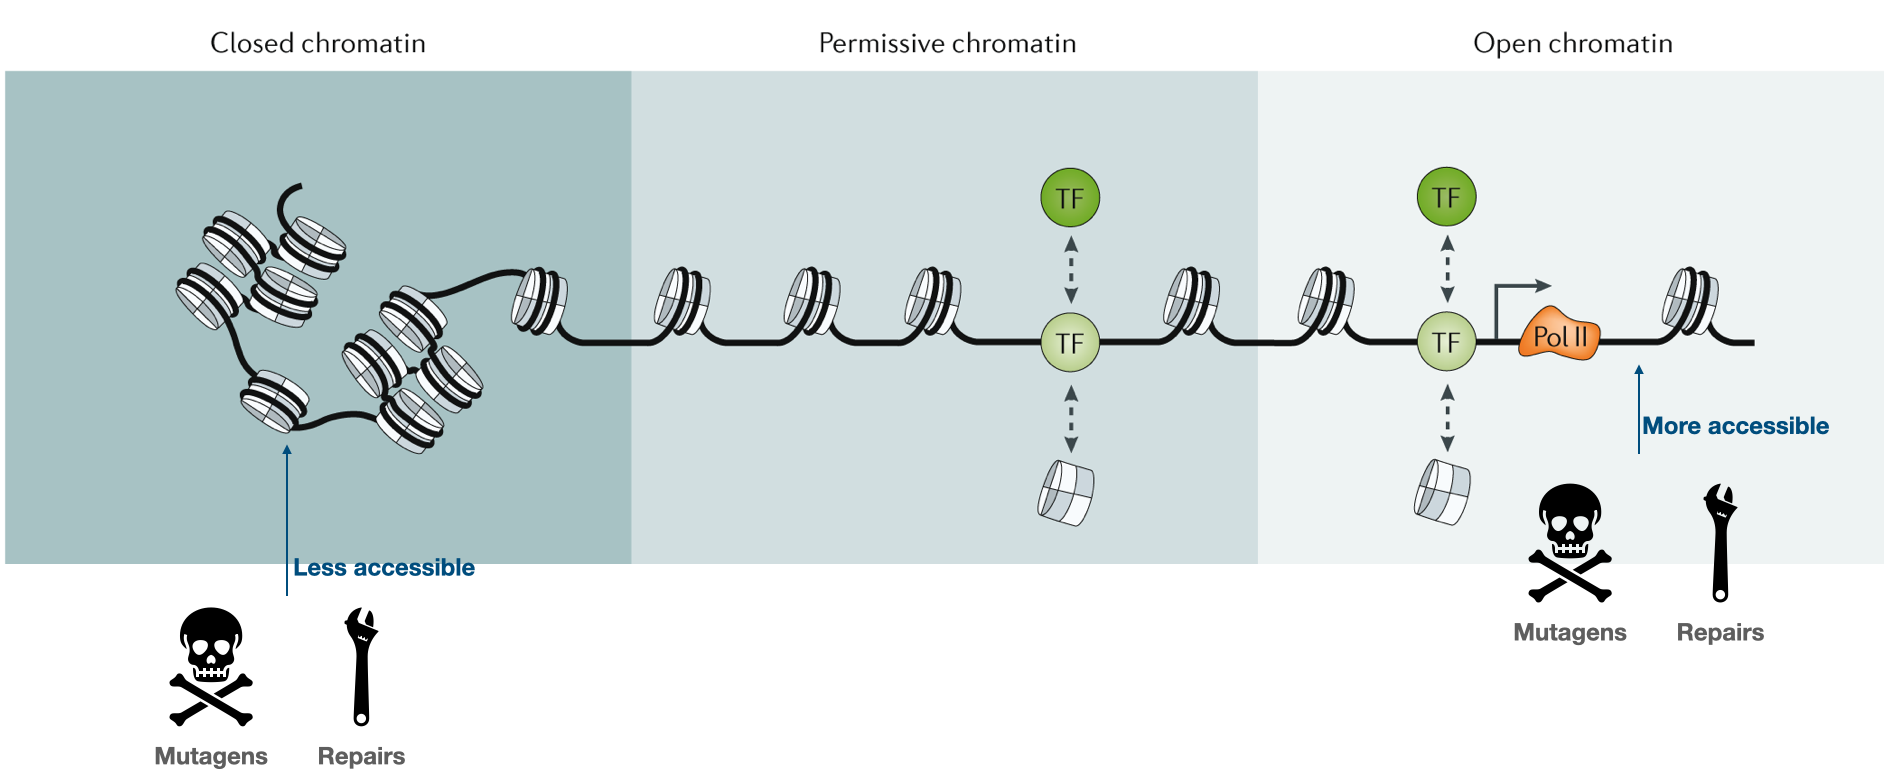
\includegraphics[scale=0.24]{graphics/chromatin_demo.png}
    \caption{\textbf{The distribution of mutations across the genome is hypothetically influenced by cell chromatin structure.} DNA in closed chromatin regions is not accessible to both mutagens and repairs, and is more prone to mutations. Different cell types have different chromatin structures as well as different repair systems, making genomic location effect (GLE) a potential factor that makes a cancer distinct from another. Figure modified from \citet{Klemm2019ChromatinEpigenome}. TF means transcription factor, Pol II means polymerase II}.
    \label{fig:chromatin_demo}
\end{figure}


To represent genomic location data, the convention is to count the number of mutations in a succession of 1 Mbp genomic segments, termed the bin method \citep{Kubler2019, Salvadores2019PassengerTumors, Chalmers2017AnalysisBurden, Salvadores2020MatchingPatterns}. However, the 1 Mbp size is picked by human, thereby imposing arbitrary boundaries to the genome. This leads to an unstable representation that is distorted when only slightly shifting the start of the bin boundaries (Figure \ref{fig:mutdistribution_demo}). As a result, my project experimented with smoothing GLE by estimating the \gls{density} at a genomic location based on the amount of data adjacent to it\footnote{details in }. The smooth representation assumes no rigid boundaries to the genome, thus less sensitive to the above pitfall. 
\begin{figure}[h!]
  \begin{minipage}[c]{0.45\textwidth}
    \caption{
      \textbf{In theory, the smoothing approach should be more robust than the bin approach.} Both panels depict the same mutation location data for a hypothetical chromosome, with the black dots below the x-axis representing the true location of mutations. By binning the genome by convention, one counts the number of mutations in each yellow bin. The obtained GLE data is then the yellow dots on top of each bin. This binned GLE data changes when shifting the bin boundaries from panel (a) to panel (b). Mutations on the right hand side of the last bin (10$^{th}$ bin) are forcefully removed. By smoothing the genome, GLE data is the same for both panels. The smoothing method also allows inclusion of mutations outside the last bins.
    } \label{fig:mutdistribution_demo}
  \end{minipage}\hfill
  \begin{minipage}[c]{0.52\textwidth}
    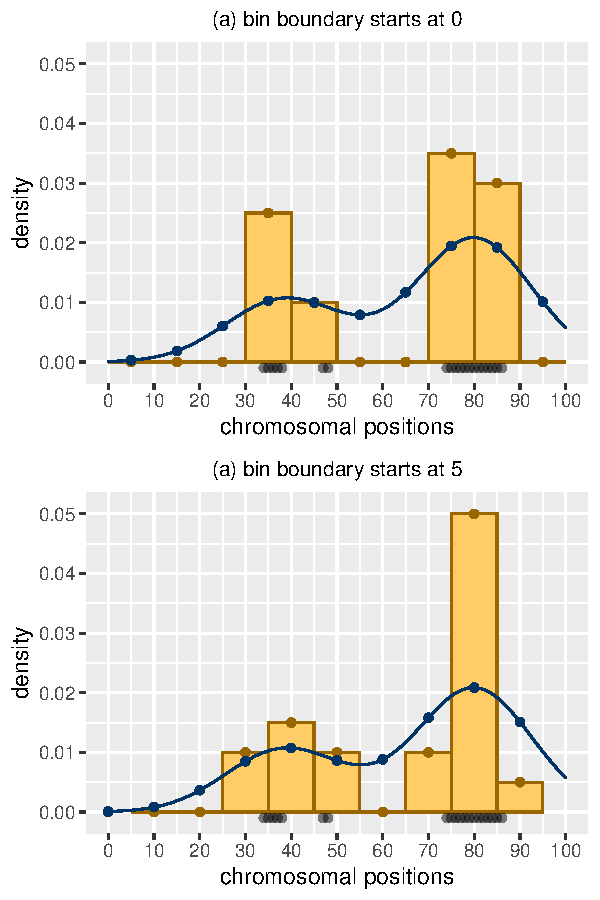
\includegraphics[width=\textwidth]{graphics/mutdistribution_demo.pdf}
  \end{minipage}
\end{figure}


\newpage
\section{Sequence context effect (SCE)}
\label{intro:sce}

Each cancer develops under the influence of different mutagenic processes, giving rise to diverse mutation compositions. These processes include, but are not limited to UV light \citep[known in skin melanoma;][]{Mohania2017}, the intrinsic cellular APOBEC deaminase activity \citep[\textit{e.g.} in B cells;][]{Kuppers2005MechanismsPathogenesis} and defective repairs \citep[\textit{e.g.} mutated \textit{BRCA} genes in breast cancer;][]{Navasardyan2021YY1TNBC}. \citet{Alexandrov2013, Alexandrov2020} showed that some processes were associated with certain mutation signatures. For instance, the signature SBS4, where there is an excess of C$\rightarrow$A mutations in the context of C[C$\rightarrow$A]A and C[C$\rightarrow$A]C over any other mutations, were only detected in tobacco smoke linked cancers such as liver hepatocellular carcinoma, lung adenocarcinoma and lung squamous cell carcinoma. As such, similar to \gls{gle}, SCE is also an important characteristic of the cancer mutation profile. 

In inspecting SCE, one should stay aware that mutations are usually closely linked with the \glspl{base} next to them \citep{Zhu2017}. A well known example is that the C$\rightarrow$T mutations tend to occur in the [C$\rightarrow$T]G context. One possible explanation is that proteins, be they repairs or mutagens, interact with DNA with high specificity (Figure \ref{fig:motif_demo}). There are two potential flaws to the standard way of representing SCE. First, while it is common practice to analyse mutation compositions in the 3-mer (3 base) context, evidence showed that bases beyond 3-mer could also influence the likelihood of mutations occurring \citep{Zhu2017,Zhu2020}. Second, base changes are generally assumed to be symmetric, meaning G$\rightarrow$A mutations are treated to be the same as their reverse complementary counterpart C$\rightarrow$T \citep{Alexandrov2013, Jiao2020}; but analyses in skin melanoma showed otherwise \citep{Zhu2017}. Accordingly, I seek to explore the information content available in different sequence context sizes, particularly outer positions to 3-mers; as well as the effect of strand symmetry/asymmetry in representing SCE.

\begin{figure}[h!]
    \centering
    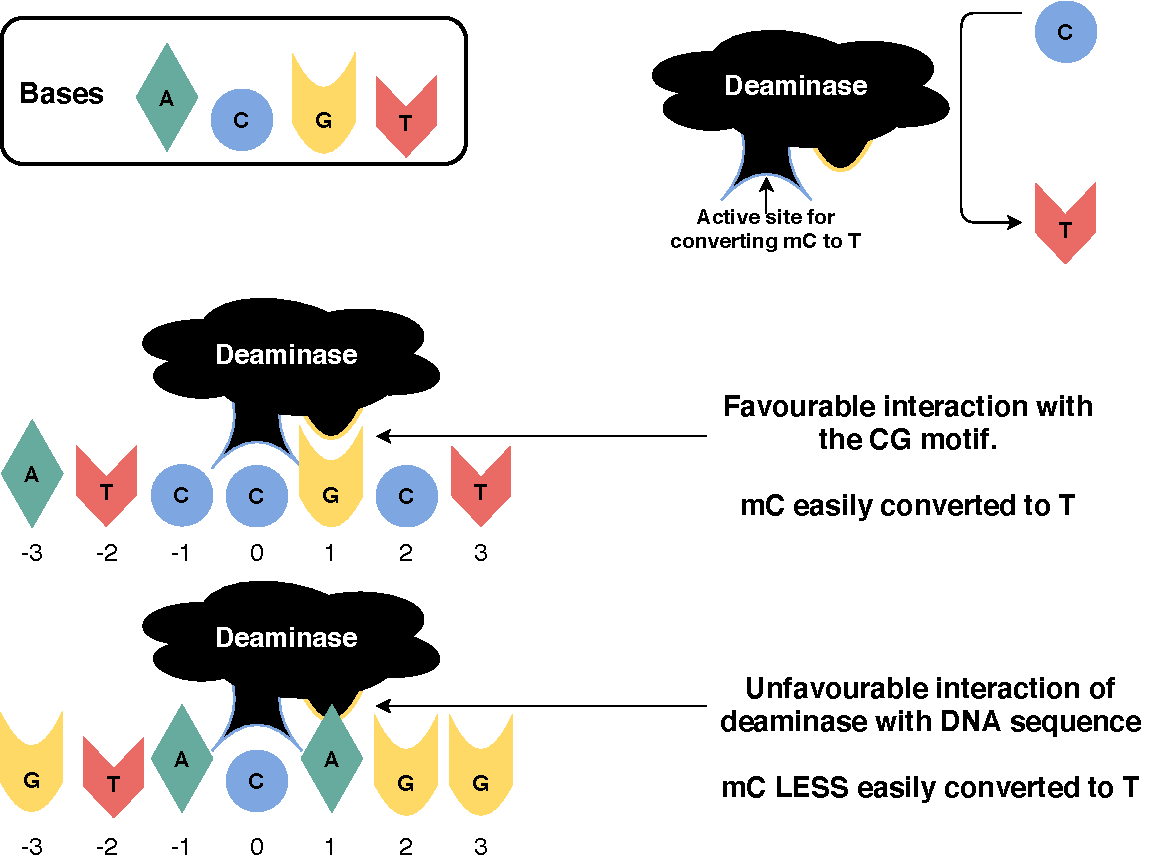
\includegraphics[scale=0.78]{graphics/motif_demo.pdf}
    \caption{\textbf{Mutations are closely linked with the bases next to them}. The schematic diagram depicts an example of hypothetical scenarios that could explain why this is the case. Here, a deaminase protein, which converts methylated C into T, interacts with DNA such that certain sequence contexts make the conversion more feasible than others. While many publications focus on the 3-mer context of mutations (pos -1, 0 and 1), which includes the base change and two bases immediately next to it, evidence shows that bases outside the 3-mer could still be influential. Part of this project seeks to explore the information content available in larger sequence contexts than 3-mers.}
    \label{fig:motif_demo}
\end{figure}


\section{Computational approaches to study GLE and SCE}
\label{intro:ml}

The release of the \gls{pcawg} project \citep{Campbell2020}, with whole genomic sequencing data for 2605 primary tumours of 38 cancer types, has made studying cancer genomics and developing cancer classification models on a large scale feasible. Nevertheless, analysing developing methods based on the PCAWG mutation data require satisfactory computational tools for data analysis. To do this, it is necessary to understand the nature of the data, which I approached on two levels, analysis on whole disease scale and classification on individual scale. First, data was investigated on the whole disease level (\gls{gle} in Chapter \ref{gle}; \gls{sce} in Chapter \ref{sce}). This means that for each cancer, mutations from all donors of that cancer were considered as a whole. This makes understanding the mutagenesis process easier as it magnifies the signals in the data if they are ``real''. Second, Chapter \ref{ml} trials different measures and data representations to train the classifiers on the individual donor level. The idea is that the more accurate the classifier, the better the assumptions imposed by its data representations could capture the nature of the data. The long term goal is to be able to apply the model to unseen data, such as the tumour genome of a new cancer patient. The analyses on two levels are complementary, in that they could be used to verify each other. Whereas whole disease analysis explores how and why a potential factor might be important, individual scale is a direct measure of how informative that factor is.  

\section{Aims and hypotheses}
\label{intro:aims}
\begin{itemize}
    \item To understand the tendency for mutations to be distributed across the genome. In particular, I seek to formally test whether mutations are distributed differently between closed and open chromatin regions; if so, how strong the bias towards closed chromatin regions is for each cancer. More importantly, I aim to investigate how informative GLE is as a result. As aforementioned, I expect if GLE is informative, then the smooth representation is the more efficient method to extract the information that the conventional bin representation.
    \item To understand how the information content available in the composition of mutations (SCE) is influenced by the base changes and their sequence contexts, especially the outer flanking positions of the 5-mer context. While it is very obvious to expect the base changes to be informative, I also expect some potential in the flanking positions. 
    \item To experiment with different measures and representations of GLE and SCE in order to improve the accuracy of the cancer classifier. This includes trialling smoothing \textit{v.s} binning GLE, different ways to integrate information from flanking bases to represent SCE, and the proposed asymmetric \textit{v.s.} the conventional symmetric representations of SCE. Finally, I examine whether combining SCE and GLE results in further accuracy improvement than each factor alone.  
\end{itemize}

\section{Key findings}
\label{intro:findings}
Overall, the project shows that both GLE and SCE are important characteristics of a cancer \gls{mut_profile}, manifesting in three aspects. First, mutations generally tend to occur in closed chromatin regions, but the degree of bias varies for different cancers. This suggests that chromatin structure is an important determinant of GLE, but there are other determining factors as well. Regardless of the driving forces, GLE was found to be distinctive of cancer types, particularly when the smoothing representation is used. Second, both components of SCE, the base changes and their sequence contexts are characteristic of cancers. Not surprisingly, information is more abundant closer to the mutations (3-mer), but the outer bases are also very informative. Additionally, there is more information in \glspl{transition} than in \glspl{transversion} for both base changes and their flanking bases. Third, when recruited to train classifiers, both GLE and SCE had a reasonably high predictive power by themselves, provided the data is represented appropriately. Specifically, as expected, smoothing GLE in any form provided a higher predictive power than binning it. Regarding SCE, incorporating the immediate neighbours within the 3-mer neighbourhood improved accuracy over the base changes alone. Moreover, classifier performance was improved when omitting the traditional assumption of strand symmetric mutations. Interestingly, while information was detected in the outer bases of the 5-mer sequence context, incorporating this information into the classifier appeared to be quite challenging. Finally, even though GLE and SCE were expected to be separate sources of information, SCE seemed to be the predominating contributor of the classifier. When training the model, I identified the problem of imbalanced design, which needs to be addressed in future research.   


\newpage

\part{Results: Exploring the features}{
    The next two chapters report the results from conventional statistical tools to analyse the two features of interest, genomic location effect (\gls{gle}) and sequence context effect (\gls{sce}), respectively. In particular, this part dwells on \textbf{whether} GLE and SCE are significantly different between different cancer types, and explores \textbf{in what way} they are different. All analyses in this part were performed on the whole disease scale. For example, data for melanoma was all the mutations aggregated from all donors diagnosed with melanoma. This acts as a basis for building the \gls{classifier} in chapter \ref{ml}.
}

\chapter{Genomic Location Effect}\label{gle}

The tendency for mutations to occur in closed \gls{chromatin} regions has been reported both in cancer and other mutagenesis processes \citep{Polak2015,Prendergast2007ChromatinGenome}. This is hypothetically because closed chromatin regions, despite being less exposed to mutagens, are harder for repair systems to reach \citep{Prendergast2007ChromatinGenome,Teng1997ExcisionSequences, Morse2002PhotoreactivationCerevisiae}. Section \ref{gle:chromatin} of this chapter shows further evidence that mutations did tend to occur in closed rather than open chromatin regions. However, the influence of chromatin structure was not discriminative between cancers. Nevertheless, section \ref{gle:bootstrap} shows that \gls{gle} was significantly different between cancers. 

\section{Mutation location was influenced by chromatin status}\label{gle:chromatin}
My analyses of GLE were motivated observations that suggests mutations tend to locate in closed chromatin regions. Figure \ref{fig:mutation_density} shows the distribution of mutations on chromosome 12 for four cancers, the rest can be found in Figure \ref{fig:apdx_mutation_density} of the appendix. The shaded DHS bars near the bottom of the plots are hypersensitive regions (open chromatin) for the original cells, which was identified by literature search and shown in Table \ref{tab:encode}. The choice to display chromosome 12 was arbitrary. By visualisation alone, it can already be seen that mutation density was greater in less dense DHS, indicating a bias towards closed chromatin regions for the cancers of interest. This pattern was particularly strong in Skin-Melanoma and Liver-HCC, and less obvious in Kidney-RCC. It is also worth noting that the chromatin structures appeared different between cancers. Looking at the density by itself, we could see a diversity in how mutations are distributed, supporting the potential of GLE in discriminating cancers. 
% \newpage

\begin{figure}[ht!]
    \begin{subfigure}{.5\textwidth}
    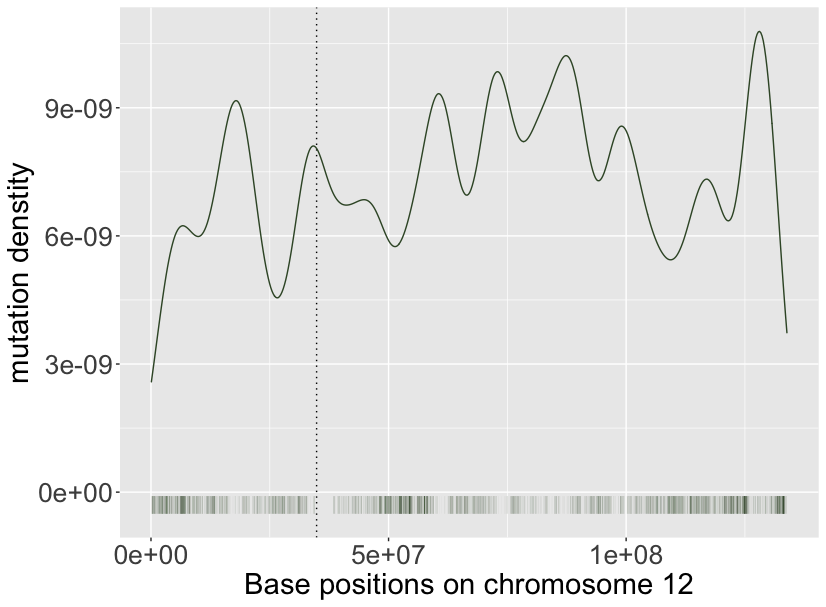
\includegraphics[width=\linewidth,height=0.7\textwidth]{graphics/mutdistribution_Skin-Melanoma.png}
    \caption{Skin-Melanoma}
    \label{fig:density_skin}
    \end{subfigure}
    ~
    \begin{subfigure}{.5\textwidth}
    
    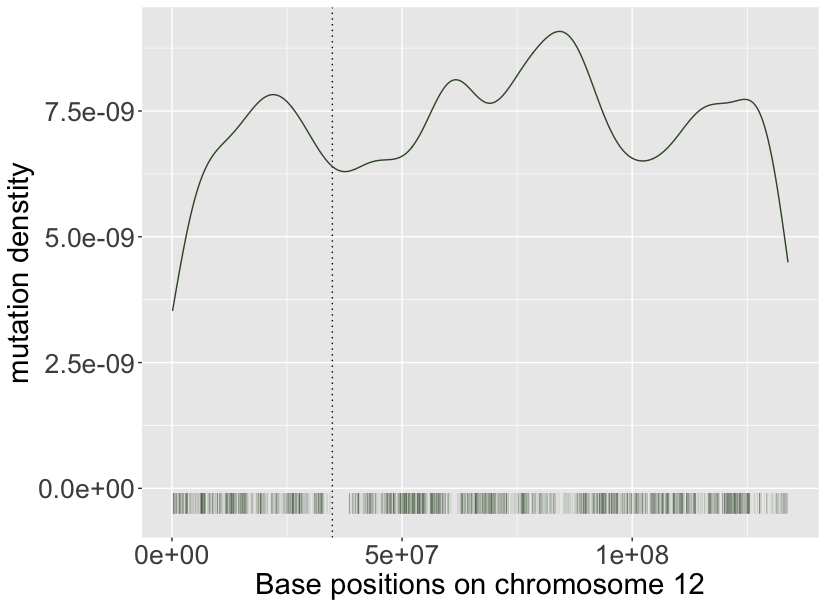
\includegraphics[width=\linewidth,height=0.7\textwidth]{graphics/mutdistribution_Kidney-RCC.png}
    \caption{Kidney-RCC}
    \label{fig:density_kidney}
    \end{subfigure} \\
    \vspace{0.5cm}
    
    \begin{subfigure}{.5\textwidth}
    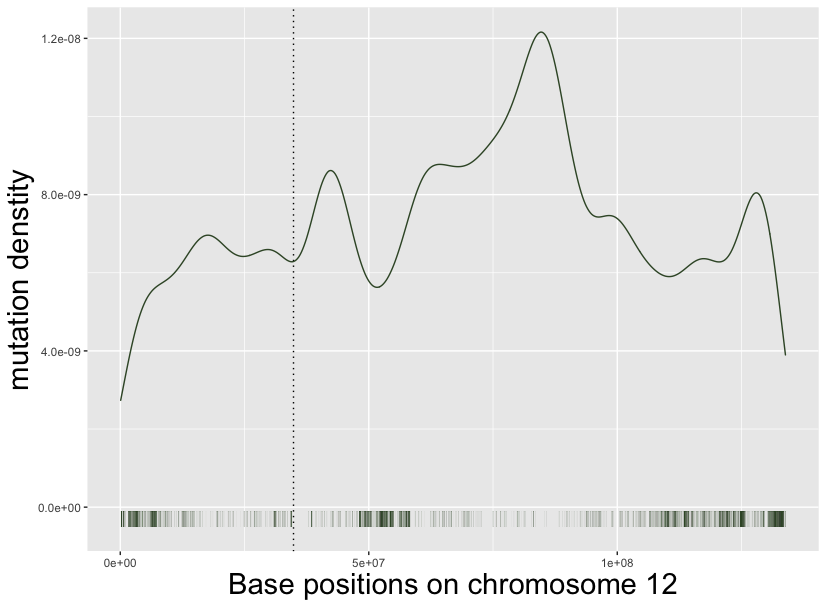
\includegraphics[width=\linewidth,height=0.7\textwidth]{graphics/mutdistribution_Liver-HCC.png}
    \caption{Liver-HCC}
    \label{fig:density_liver}
    \end{subfigure}
    ~
    \begin{subfigure}{.5\textwidth}
    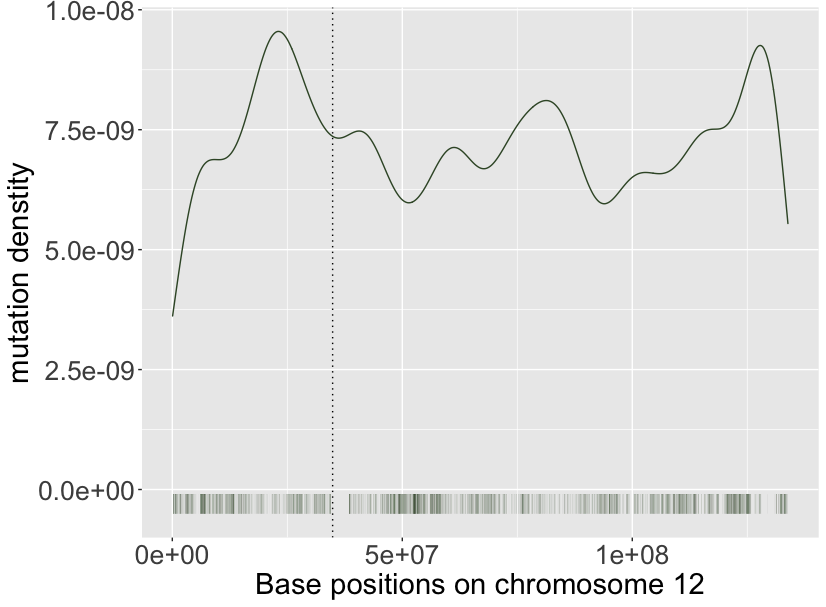
\includegraphics[width=\linewidth,height=0.7\textwidth]{graphics/mutdistribution_Panc-AdenoCA.png}
    \caption{Panc-AdenoCA}
    \label{fig:density_panc_adenoca}
    \end{subfigure} \\
    \caption{\textbf{Mutations tend to be found in closed chromatin regions.} Different cancers differ in the distribution of mutations across the genome. Here chromosome 12 is shown. (a) Skin-Melanoma (b) Kidney-RCC (c) Liver-HCC (d) Panc-AdenoCA, the other cancers are shown in Figure \ref{fig:apdx_mutation_density}. The shaded bars below the x-axis indicate open chromatin regions, the gaps indicate closed chromatin regions of the original cell types. The vertical dotted line indicates the position of the centromere.}
    \label{fig:mutation_density}
\end{figure}

\subsection{Some cancers were more similar than others in terms of chromatin structures}\label{gle:pca}
In investigating whether the diversity in GLE is influenced by chromatin structure, one factor worth considering is how cancers relate to each other by the chromatin structure of their original cells to begin with. To compute the difference between the DHS of two original cell types, I identified the span of the intersection of their open chromatin regions and converted it into a distance (details in Methods \ref{methods:encode_pca}). The distance between every pair of cells allows calculating and visualising their relative coordinates using multidimensional scaling. Figure \ref{fig:encode_pca} shows the three most informative dimensions (PC1, PC2 and PC3) for the relationship between the original cells of cancers. Melanocyte and hepatocyte had the most distinct chromatin structures as they were relatively far away from the other cell types. On the other hand, prostate epithelium (ProstEpi) and exocrine cells of the pancreatic duct (PancDuct) were very close with respect to DHS on both panels.

% \begin{figure}[h!]
%     \begin{subfigure}{.5\textwidth}
%     \centering
%     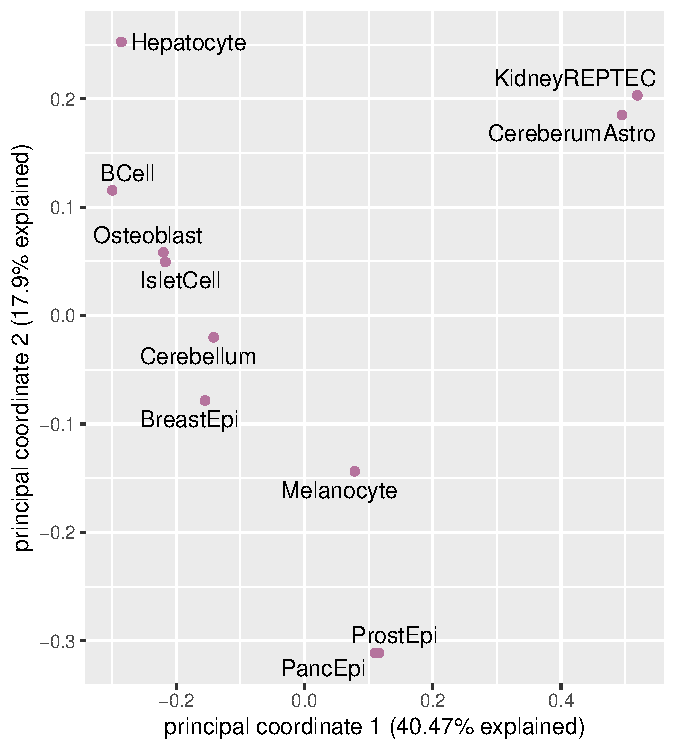
\includegraphics[scale=0.7]{graphics/encode_pca_1_2.pdf}
%     \caption{PC2 \textit{v.s.} PC1}
%     \end{subfigure}
%     ~
%     \begin{subfigure}{.5\textwidth}
%     \centering
%     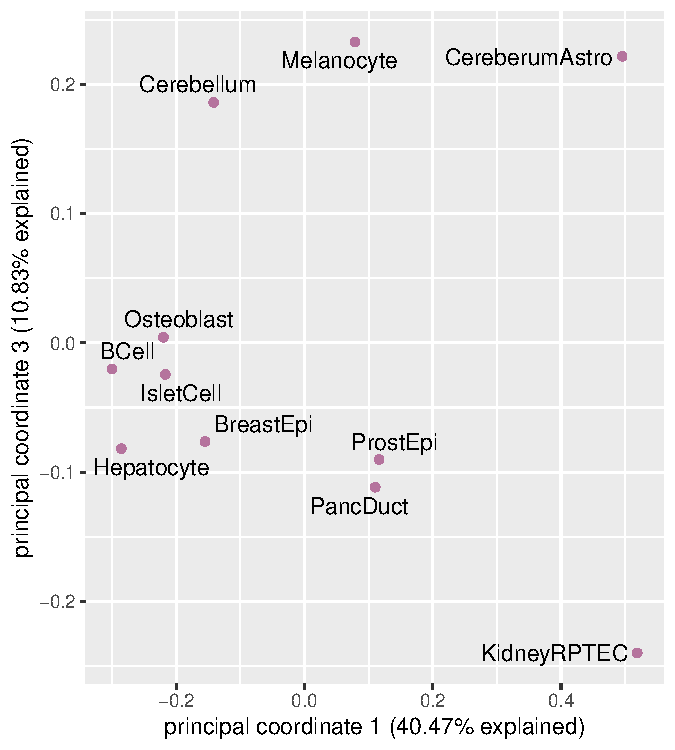
\includegraphics[scale=0.7]{graphics/encode_pca_1_3.pdf}
%     \caption{PC3 \textit{v.s.} PC1}
%     \end{subfigure} \\
%     \caption{\textbf{PCA}.}
%     \label{fig:encode_pca}
% \end{figure}

\begin{figure}[h!]
  \begin{minipage}[c]{\textwidth}
    \begin{subfigure}{.5\textwidth}
    \centering
    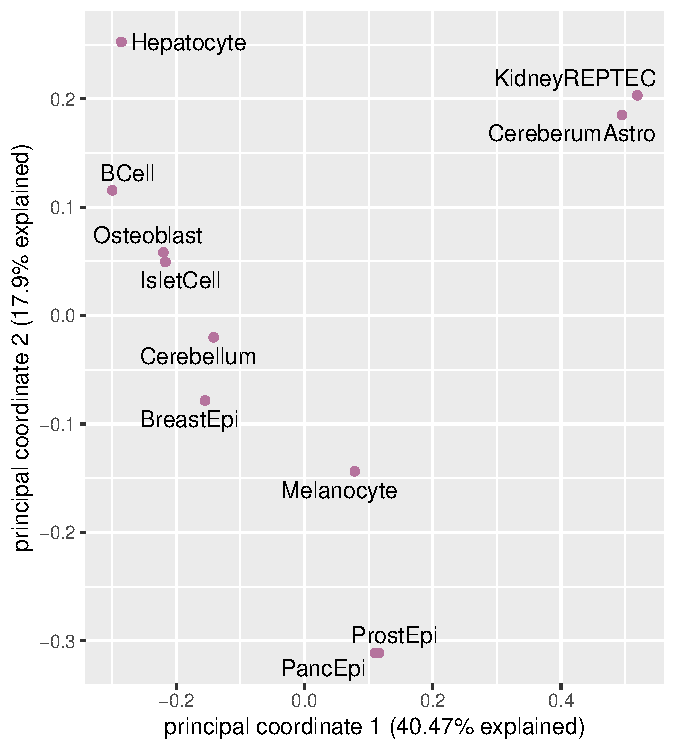
\includegraphics[scale=0.7]{graphics/encode_pca_1_2.pdf}
    \caption{PC2 \textit{v.s.} PC1}
    \end{subfigure}
    ~
    \begin{subfigure}{.5\textwidth}
    \centering
    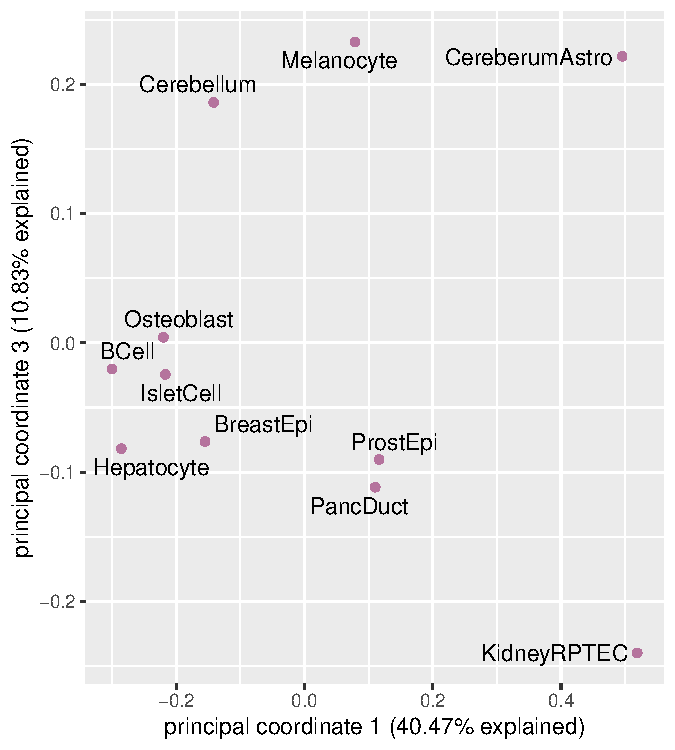
\includegraphics[scale=0.7]{graphics/encode_pca_1_3.pdf}
    \caption{PC3 \textit{v.s.} PC1}
    \end{subfigure} \\
  \end{minipage}\hfill
  \vspace{1cm}
  
  \begin{minipage}[c]{\textwidth}
    \centering
    \begin{tabulary}{\textwidth}{ ll }
    \toprule
    \textbf{Original cell abbreviation} & \bf{Cancer Type}  \\
    \toprule
    Osteoblast & Osteosarcoma \\
    
    BreastEpi & Breast-AdenoCa \\
    
    Cerebellum &  CNS-Medullo  \\
    
    CereberumAstro & CNS-PiloAstro \\
    
    KidneyRPTEC & Kidney-RCC \\
    
    Hepatocyte & Liver-HCC \\
    
    BCell & Lymph-BNHL, Lymph-CLL \\
    
    PancDuct & Panc-AdenoCa \\
    
    IsletCell & Panc-Endocrine \\
    
    ProstEpi & Prost-AdenoCa \\
    
    Melanocyte & Skin-Melanoma \\
    \bottomrule
    
    \end{tabulary}
    
    % . DHS data for these cells is downloaded from either \href{https://genome.ucsc.edu/cgi-bin/hgFileUi?db=hg19&g=wgEncodeOpenChromDnase}{Duke} or \href{https://genome.ucsc.edu/cgi-bin/hgFileUi?db=hg19&g=wgEncodeUwDnase}{UW} project
  \end{minipage}\hfill
  \vspace{0.5cm}
  
  \begin{minipage}[c]{\textwidth}
    \caption{
      \textbf{Some cancers were more related in terms of chromatin structures than others.} Here, I visualised the relative coordinates of the original cell types for cancers on the most informative dimensions (principle coordinates, PC). This was done by multidimensional scaling of the pairwise distance between cell types. The distance between two cell types was computed based on the intersection between their open chromatin regions. 
    } \label{fig:encode_pca}
  \end{minipage}
\end{figure}


\subsection{Open and closed chromatin regions have significantly different mutation rates}\label{gle:g}
Having visualised the tendency of mutation location and the relationship between the chromatin structures of the original cells, I performed a hypothesis test to confirm whether there was a difference in how mutations are distributed between open and closed chromatin regions. This was achieved using the G-test of independence (details in Methods \ref{methods:chromatin}). The p-values obtained from this were adjusted using Bonferroni multiple test correction (Table \ref{tab:g-test}, the raw inputs can be found in Appendix \ref{apdx:g-test}). To begin with, the size of the regions identified as open chromatin was considerably tiny compared to that of closed chromatin regions. Keeping that in mind, we can see that most cancers had significantly different mutation rates between open and closed chromatin regions, except CNS-PiloAstro and Panc-Endocrine. Note that these two cancers had small to modest numbers of mutations. While no direct correlation between p-values and number of mutations could be detected, no cancers with less than 1 million mutations gave a p-value $>10^{-100}$. Our conclusion remains that mutation location is not random between open and closed chromatin regions, but this implies the impact of the number of mutations on the power of the test. 

% latex table generated in R 4.1.0 by xtable 1.8-4 package
% Tue Oct 19 08:53:20 2021
\begin{table}[h]
\centering
\caption{\textbf{The chance of mutations occurring are significantly different between closed and open regions for most cancers.} The table presents }
\label{tab:g-test}
\begin{tabular}{lrr}
  \toprule
 \textbf{Disease} & \textbf{$\hat{p}$-value} & \textbf{Number of mutations} \\ 
  \hline
 Bone-Osteosarc & 5.66 $\times 10^{-35}$ & 166845 \\ 
 Breast-AdenoCa & 1.33 $\times 10^{-10}$ & 713855 \\ 
 CNS-Medullo & 2.46 $\times 10^{-34}$ & 209997 \\ 
 CNS-PiloAstro & 1.00 & 22020 \\ 
 Kidney-RCC & 2.60 $\times 10^{-06}$ & 531886 \\ 
 Liver-HCC & $<10^{-100}$ & 3321521 \\ 
 Lymph-BNHL & $<10^{-100}$ & 1124881 \\ 
 Lymph-CLL & $<10^{-100}$ & 226242 \\ 
 Panc-AdenoCA & $<10^{-100}$ & 1675781 \\ 
 Panc-Endocrine & 8.82 $\times 10^{-02}$ & 258564 \\ 
 Prost-AdenoCA & 5.49 $\times 10^{-90}$ & 1000496 \\ 
 Skin-Melanoma & $<10^{-100}$ & 7770980 \\ 
   \bottomrule
\end{tabular}
\end{table}

\subsection{Mutations were typically biased towards closed regions}\label{gle:or}
Complementary to the G-tests, which suggested that the difference in mutation location were statistically significance between closed and open chromatin regions, I computed the odds ratio ($OR$), which measures the direction of this difference. From equation \ref{eq:or} (Methods \ref{methods:chromatin}), $OR$ compares the ratios of mutated over non-mutated positions between closed and open chromatin regions. An $OR>1$ indicates a bias towards closed regions, and an $OR<1$ indicates a bias towards open regions. For each cancer, I estimated the standard error of $OR$'s using jackknife, where one donor was removed to obtain a pseudo-value for $OR$. The standard errors of the resulting $OR^{pseudo}$'s were the jackknifed standard error for $OR$. The results are shown in Figure \ref{fig:or_jackknifed}.

\begin{figure}[h!]
    \centering
    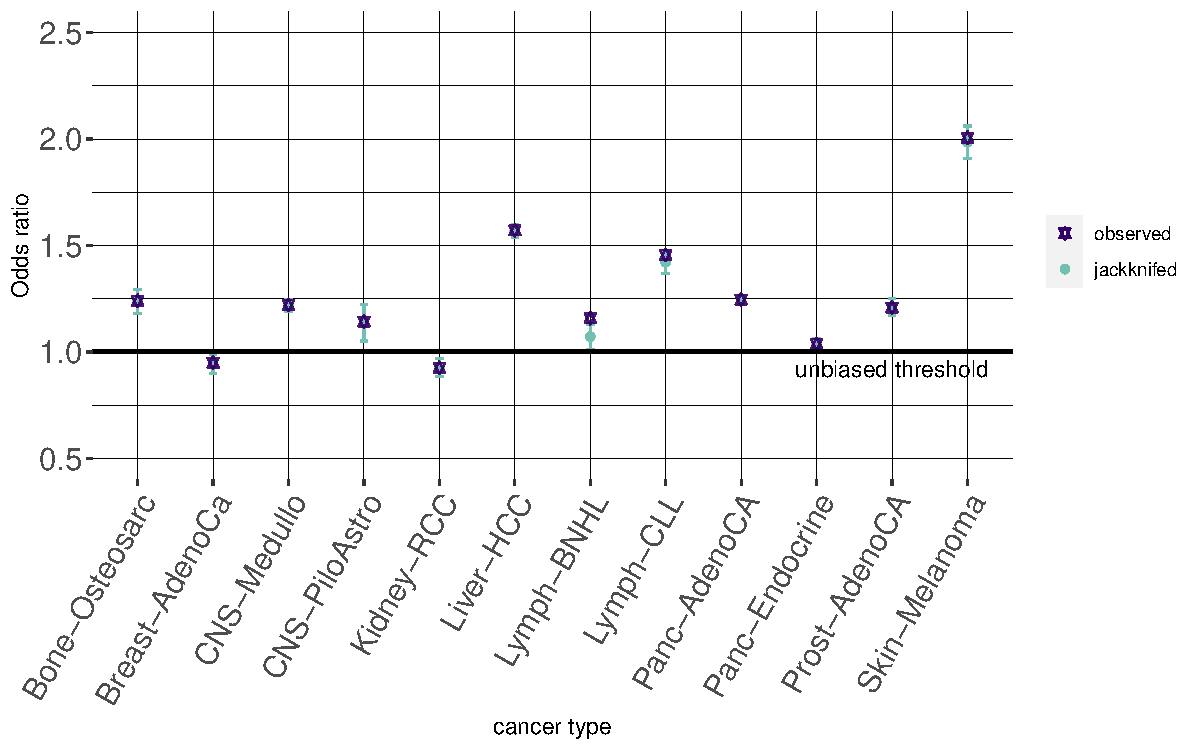
\includegraphics[scale=0.8]{graphics/jackknife_OR.pdf}
    \caption{\textbf{Mutations tend to occur in closed chromatin regions according to the odds ratio ($OR$) statistic}. $OR>1$ indicates a bias towards towards closed regions, and $OR<1$ indicates the opposite. Error bars are the standard errors of the jackknifed sample. The green circles are the means of the jackknifed pseudo-values. The purple stars are the observed $OR$.}
    \label{fig:or_jackknifed}
\end{figure}


Overall, mutations preferred to locate in closed chromatin regions, especially for Skin-Melanoma ($OR=2$). However, this bias varied between cancers. In addition, there are three other intriguing features. First, Breast-AdenoCa and Kidney-RCC had $OR<1$. Their p-values from the G-test showed a significant difference between closed and open regions, suggesting that the preference for open regions was not due to noise. On the density plots (Figures \ref{fig:mutation_density} and \ref{fig:apdx_mutation_density}), mutations still peaked at closed chromatin regions, but less clear than for example Skin-Melanoma. Second, the departure of the observed $OR$ from the mean pseudo-values in Lymph-BNHL and Lymph-CLL suggests an abnormality in these cases. This abnormality could be due to the large variance of GLE in donors with these cancers. However, it could also come from the uncertainty in identifying the original cells (B cells for both cancers, discussed in \ref{}). Third, CNS-PiloAstro had the largest standard error of $OR$. Again, this might be because its small number of mutations lowered the signal to noise ratio compared to other cancers, which is consistent with the G-test results. Regarding reliability, empirically, $OR$ seemed more robust to the number of mutations than G-test. Mathematically, it accounts for the imbalance in the size of open \textit{v.s.} closed chromatin regions. However, we need to be vigilant about the existence of this imbalance.

\subsection{Chromatin structure was influential but not discriminative}\label{gle:mixed_or}

In this subsection, I evaluated the appropriateness of $OR$ given the imbalance between the size of open and closed chromatin regions and the potential of $OR$ in discriminating cancers. The evaluation was done by calculating the $OR$'s with mislabelled DHS data. That is, mislabelled $OR$ was calculated by sorting a cancer's mutation data based on other cancers' DHS data rather than its own (Methods \ref{methods:chromatin}). 

The impact of imbalanced DHS was assessed in Figure \ref{fig:mixed_or_violin}. Specifically, I examined whether the very large size of closed chromatin regions rather than its biological properties made mutations in closed regions more likely than in open regions. If $OR$ was sensitive to the imbalance, then each violin should have had a distinctive value. A good example to illustrate this involves Skin-Melanoma and Kidney-RCC, whose ratios of closed over open chromatin regions were 65:1 and 115:1 in their original cells' DHS, respectively (Table \ref{fig:tab_g-test_contingency}). If $OR$ was sensitive, then it should have always been higher in Kidney-RCC than Skin-Melanoma, no matter what mutation data was used. This was not the case. $OR$ range was approximately the same for Kidney-RCC and Skin-Melanoma, which suggests that the effect of the imbalance in DHS data was mild for the purpose of this project.

However, it is curious that $OR$ was not typically the highest when DHS data of the correctly labelled cancer was used. This was further reinforced in Figure \ref{fig:mixed_or_heatmap}. Each column of Figure \ref{fig:mixed_or_heatmap}, representing a cancer whose DHS data was used, was coloured with respect to the rank of $OR$'s for cancers with mutation data. It is worth noting that Figure \ref{fig:mixed_or_violin} is basically the violin plot by the columns of Figure \ref{fig:mixed_or_heatmap}, where each violin contains the $OR$'s with mislabelled mutation data and a fixed DHS data. Mutation data for Skin-Melanoma almost always produced one of the highest $OR$'s, irrespective of the cancer types used for DHS data. Another way to view this is to use the violin plot by the rows rather than columns of the heatmap, where DHS data is mislabelled (Figure \ref{fig:mixed_or_byrow}). Contrary to plotting $OR$ against mislabelled mutation data (DHS data being the determinant), plotting $OR$ against mislabelled DHS data (mutation data being the determinant) showed distinctive ranges of $OR$ for most cancers, except Liver-HCC. This means that $OR$ was determined by the properties of mutation data instead of DHS data. Accordingly, chromatin structure, in the form of $OR$ is indicative of mutation location, but it is unlikely to be the main determinant of whether GLE differs between cancers. One possible explanation is the similarities in the DHS data of the original cells.

\begin{figure}[ht!]
    \begin{subfigure}{\textwidth}
    \centering
    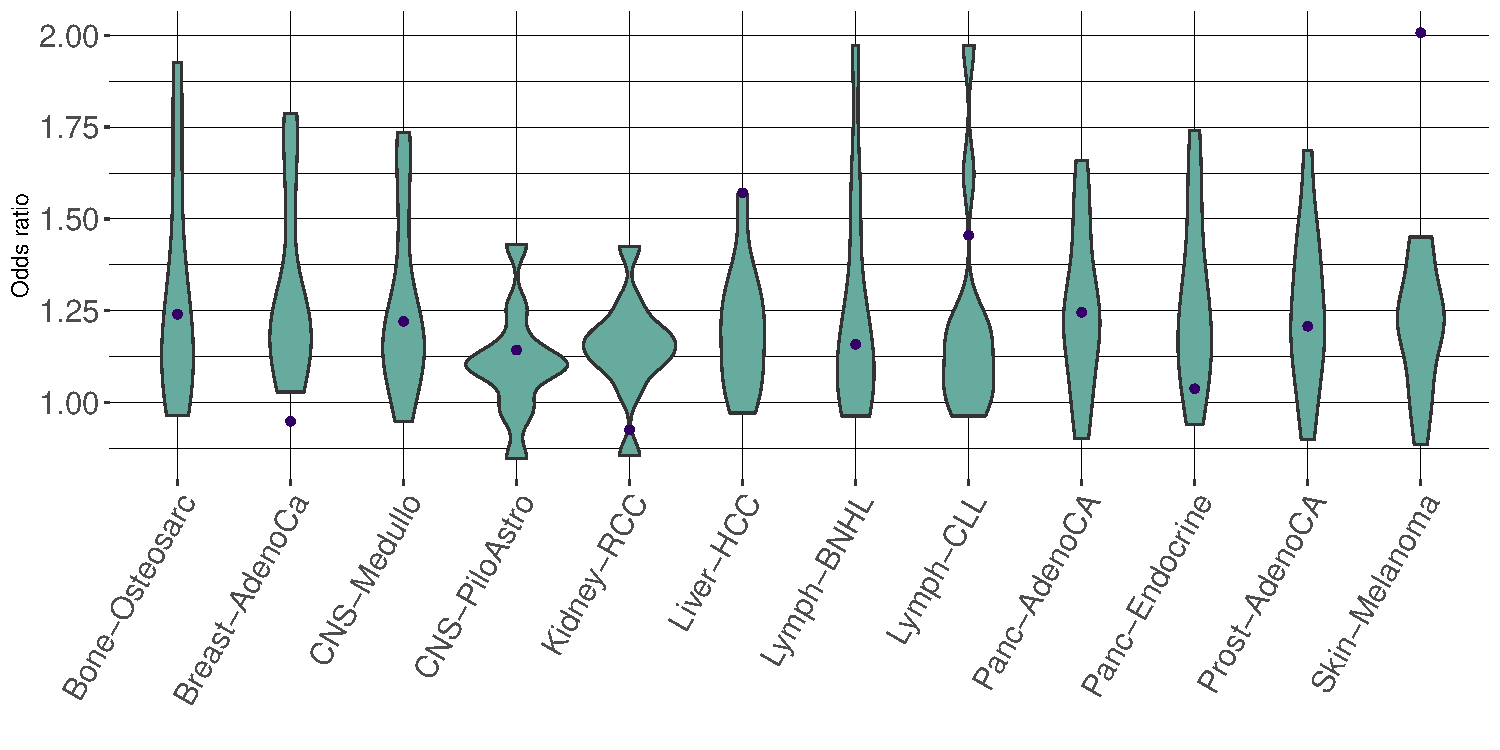
\includegraphics[scale=0.5]{graphics/mixed_or_violin.pdf}
    \caption{The impact of imbalanced DHS data on $OR$ is mild}
    \label{fig:mixed_or_violin}
    \end{subfigure} \\
    
    \vspace{0.3cm}
    \begin{subfigure}{\textwidth}
    \centering
    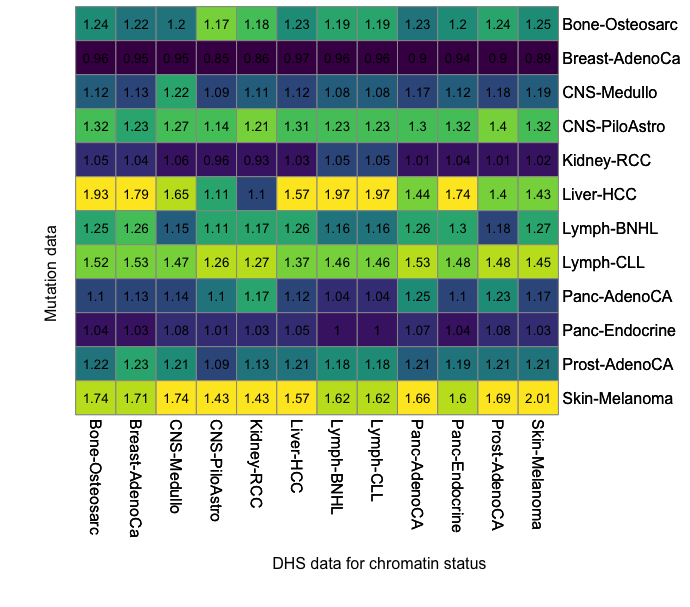
\includegraphics[scale=0.52]{graphics/mixed_or_heatmap.png}
    \caption{Chromatin structure is not discriminative of cancers}
    \label{fig:mixed_or_heatmap}
    \end{subfigure} 
\caption{}
    % \caption{\textbf{(a) The bias of mutations towards closed regions was not due to their large size compared to open regions but (b) this bias was unlikely the reason why GLE differs between cancers.} This figure shows an experiment where $OR$'s were calculated by cross-matching DHS data with mutation data of different cancers. In (a), the x-axis is the cancers whose DHS data was used, the y-axis is the distribution of $OR$ with mislabelled mutation data, with the purple dot indicating when mutation data of the correctly labelled cancer was used. In (b), the column labels are the cancers whose DHS data was used, the row labels are the cancers whose mutation data was used; each column is coloured by the rank of $OR$'s, brighter colours come from cancers whose mutation data produced the greater $OR$'s.}
    \label{fig:mixed_or}
\end{figure}

\section{GLE was significantly different between cancers}\label{gle:bootstrap}
Previously, we observed different patterns of GLE for different cancers by visualisation (Figure \ref{fig:mutation_density}). In this section, I investigated whether the difference is statistically significant and what data representations are optimal for GLE. For each pair of cancers, I used a bootstrap hypothesis test for whether their GLE are significantly different. The bootstrap involved comparing the observed distance to 1000 distances simulated under the null that assumed there was no difference between the pair, from which a p-value can be obtained (details in Methods \ref{methods:bootstrap}).

In addition to trialling the conventional bin representation \textit{v.s.} the proposed smooth representation, I also trialled two distance measures, Euclidean and Wasserstein, to see which representation/measure could best discriminate cancers. I trialled the Euclidean distance because it is the most widely used distance measures, and Wasserstein distance because it matches the nature of GLE data, which is the spatial distribution of mutations across the genome. The detailed techniques for the two distances are described in Methods \ref{methods:bootstrap} but the fundamental difference between them can be found in Methods Figure \ref{fig:wasserstein_demo}. Briefly, the Euclidean distance is rigidly the point-wise difference between two vectors whereas the Wasserstein distance allows comparing points at different coordinates of the two vectors. I reported the raw p-values rather than recruiting multiple test correction because the true purpose of this section was to detect signals in the data and to compare the performance between representations. Therefore, it was not particularly meaningful to set a rigid significance threshold. From Figure \ref{fig:gle_bootstrap}, across both representations and distance measures, GLE was generally very different for all cancer pairs. The smooth representation was more likely to output more significant p-values, with only two pairs at p-values $>0.001$ for Wasserstein and no pairs for Euclidean distance. Note that the p-value matrices in Figure \ref{fig:gle_bootstrap} are symmetric. In addition, the most common cancer with p-value $>0.001$ was CNS-PiloAstro, which might be due to its small sample size, as in the case with the G-test and the $OR$. 

\begin{figure}[ht!]
    \begin{subfigure}{.5\textwidth}
    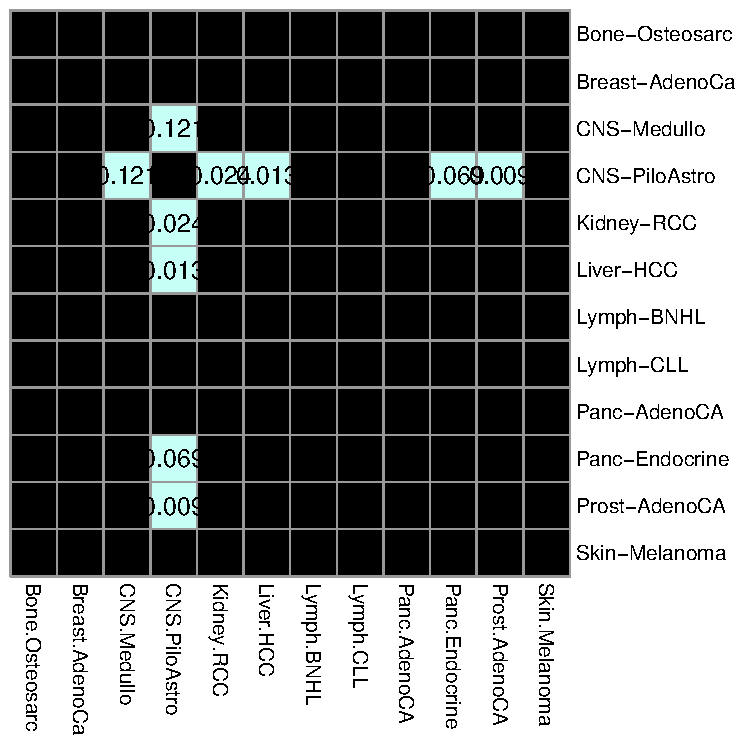
\includegraphics[scale=0.7]{graphics/bootstrap_bins_euclidean.pdf}
    \caption{Bins/Euclidean}
    \label{fig:bootstrap_bins_euclidean}
    \end{subfigure}
    ~
    \begin{subfigure}{.5\textwidth}
    
    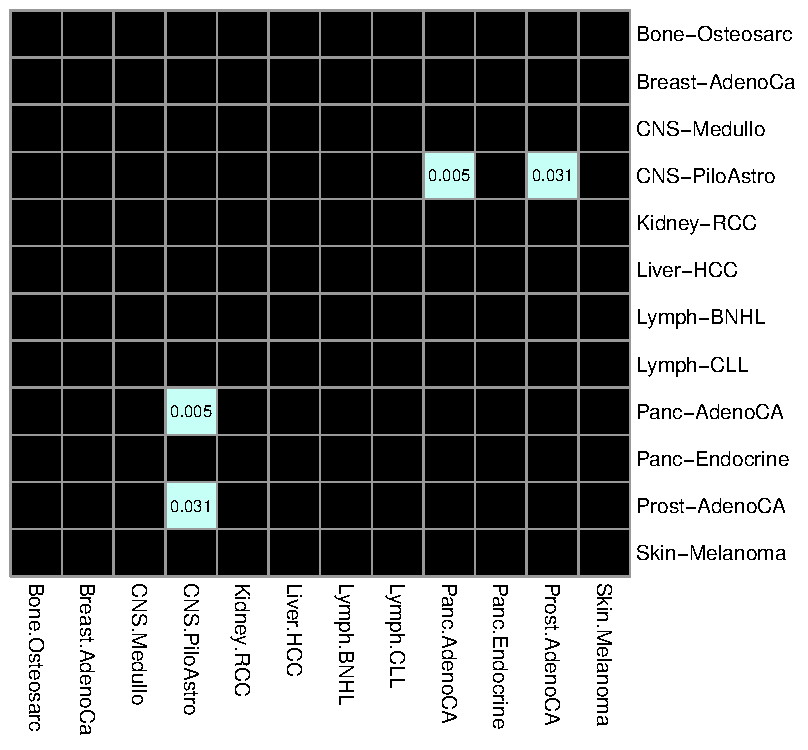
\includegraphics[scale=0.7]{graphics/bootstrap_bins_wasserstein.pdf}
    \caption{Bins/Wasserstein}
    \label{fig:bootstrap_bins_wasserstein}
    \end{subfigure} \\
    \vspace{0.5cm}
    
    \begin{subfigure}{.5\textwidth}
    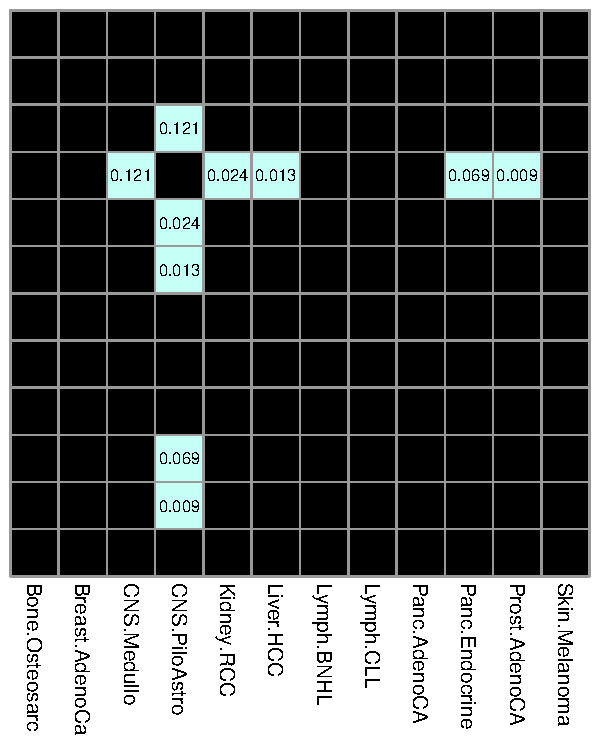
\includegraphics[width=\linewidth,height=0.7\textwidth]{graphics/bootstrap_smooth_euclidean.pdf}
    \caption{Smooth/Euclidean}
    \label{fig:bootstrap_smooth_euclidean}
    \end{subfigure}
    ~
    \begin{subfigure}{.5\textwidth}
    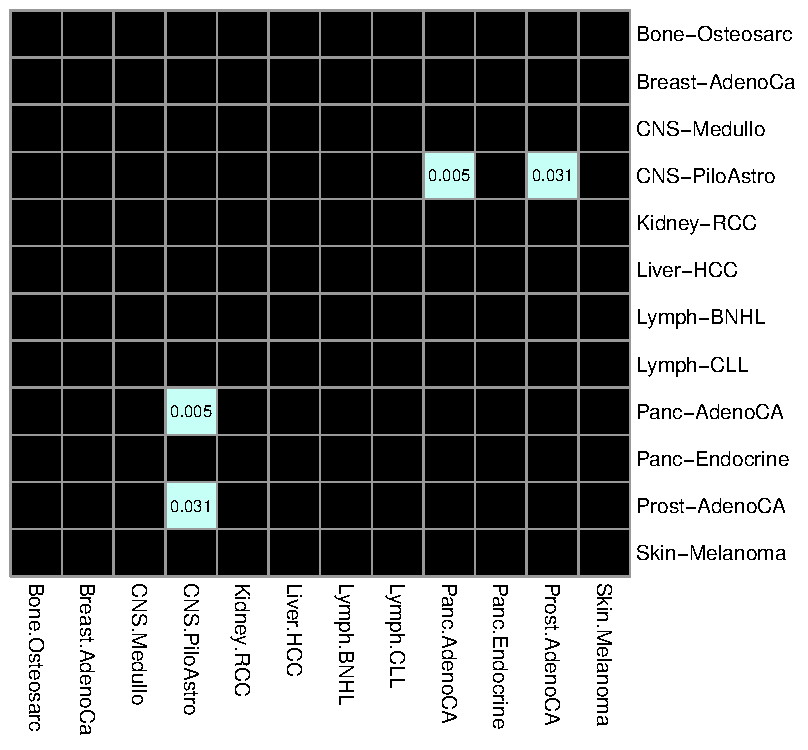
\includegraphics[width=\linewidth,height=0.7\textwidth]{graphics/bootstrap_smooth_wasserstein.pdf}
    \caption{Smooth/Wasserstein}
    \label{fig:smooth_wasserstein}
    \end{subfigure} \\
    
    \caption{\textbf{GLE was generally significantly different between cancers according to bootstrap hypothesis test using (a) Bin/Euclidean, (b) Bin/Wasserstein, (c) Smooth/Euclidean, (d) Smooth/Wasserstein.} No multiple test correction was applied. All estimated p-values were $<0.001$ unless otherwise specified.}
    \label{fig:bootstrap}
\end{figure}

\section{Chapter summary}
Overall, the analysis of GLE shows that GLE is an important characteristic of a cancer mutation profile. In particular, GLE was influenced by chromatin structure and it differed between cancers, but the former was unlikely to be causal of the latter. In section \ref{gle:chromatin}, I showed that mutations tended to occur in closed chromatin regions compared to open chromatin regions by visualisation and by formal statistical techniques. These techniques include the G-test of independence, which showed that the distribution of mutations were significantly different between open and closed regions (subsection \ref{gle:g}) and the $OR$ statistic, which showed that mutations were biased towards closed chromatin regions (subsection \ref{gle:or}). The mislabelling experiment in subsection \ref{gle:mixed_or} shows that $OR$ is an appropriate measure of mutations bias in that it was not impacted by the imbalanced sizes between open and closed chromatin regions. However, subsection \ref{gle:mixed_or} also showed that chromatin structure was unlikely to determine whether GLE differed between cancers or not. In section \ref{gle:bootstrap}, using hypothesis tests by bootstrapping, GLE was shown to significantly differ between cancers, irrespective of the driving mechanisms. More importantly, smoothing GLE was demonstrated to be better at extracting information from mutation location than binning for both Euclidean and Wasserstein distances because it produced more significant p-values for differentiating cancers.

\chapter{Sequence Context Effect}\label{sce}

Different cancers develop under the influence of different conditions, especially mutagens and repair systems, thus each cancer type possesses a distinctive mutation composition. Regarding individual mutation, each base change is closely integrated with the bases next to it \citep{Zhu2017,Zhu2020,Vinson2012CGMethylation}. The question is whether flanking bases beyond 3-mers, specifically positions -2 \& +2, have an influence on whether the mutations occur. Using a measure of information richness, \gls{re}, this chapter demonstrates the importance of both the composition of base changes and their flanking bases in characterising the carcinogenesis pattern, with evidence of strand symmetry. Above all, the chapter shows that the \gls{sce} is not just contributed by immediate flanking bases (\textit{i.e.} 3-mers). Rather, there is certain value in factoring larger sequence contexts into analysing cancer mutation composition.

\section{Base substitutions are indicative of cancers}
SCE consists of two components, the middle base substitutions and the flanking bases. This section focuses on the first component.

\subsection{Base substitutions are a rich source of information}
To explore the patterns of base substitutions and its potential contribution to SCE, I calculated $RE$'s for each mutation of every cancer. $RE$'s are essentially the information which the null cannot capture. Here, the null assumed that all mutations with the same wildtype occurred at the same rates (details in \ref{methods:re}). I plotted $RE$ as sequence logos in Figures \ref{fig:spectra} and \ref{fig:apdx_spectra}, where the height of the letter is the $RE$ of the mutation and its orientation dictates whether the mutation is in excess (up) or deficit (down). We are interested in the shape of the sequence logos. Three features stand out from the plots. First, base substitutions were strand symmetric for all cancers because the plots are point symmetric. That is, $RE$'s are similar for reverse complementary mutations (\textit{e.g.} C$\rightarrow$T and G$\rightarrow$A). Second, the heights of the up-oriented letters for transitions signifies that they were more abundant than transversions. Third, by visualisation, the patterns of base substitutions were very diverse. For example, Skin-Melanoma were predominated by C$\rightarrow$T, but this was not necessarily true in other cancers, such as Liver-HCC. Indeed, Liver-HCC was more strongly0 characterised by the A$\rightarrow$G transitions.

\begin{figure}[ht!]
    \begin{subfigure}{.5\textwidth}
    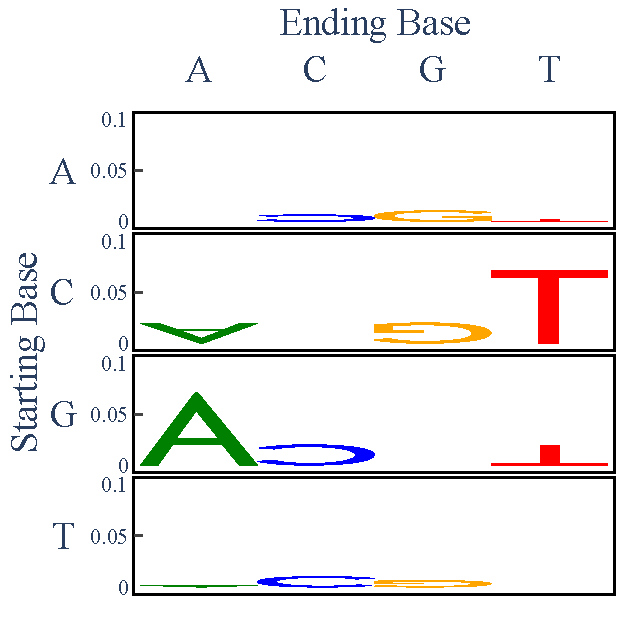
\includegraphics[scale=0.7]{graphics/spectra_Skin-Melanoma.pdf}
    \caption{Skin-Melanoma}
    \label{fig:spectra_skin}
    \end{subfigure}
    ~
    \begin{subfigure}{.5\textwidth}
    
    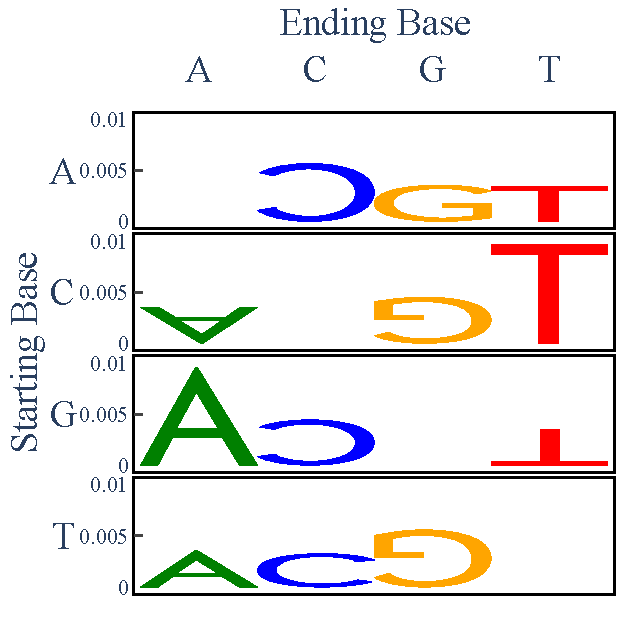
\includegraphics[scale=0.7]{graphics/spectra_Kidney-RCC.pdf}
    \caption{Kidney-RCC}
    \label{fig:spectra_kidney}
    \end{subfigure} \\
    \vspace{0.5cm}
    
    \begin{subfigure}{.5\textwidth}
    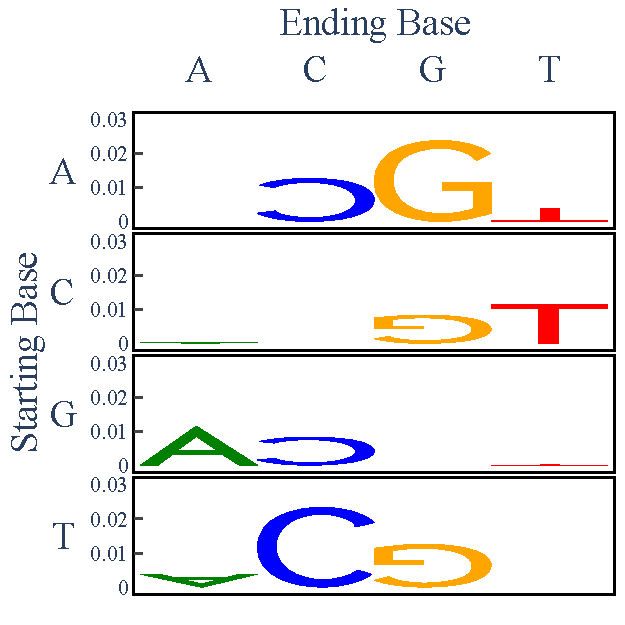
\includegraphics[scale=0.7]{graphics/spectra_Liver-HCC.pdf}
    \caption{Liver-HCC}
    \label{fig:spectra_liver}
    \end{subfigure}
    ~
    \begin{subfigure}{.5\textwidth}
    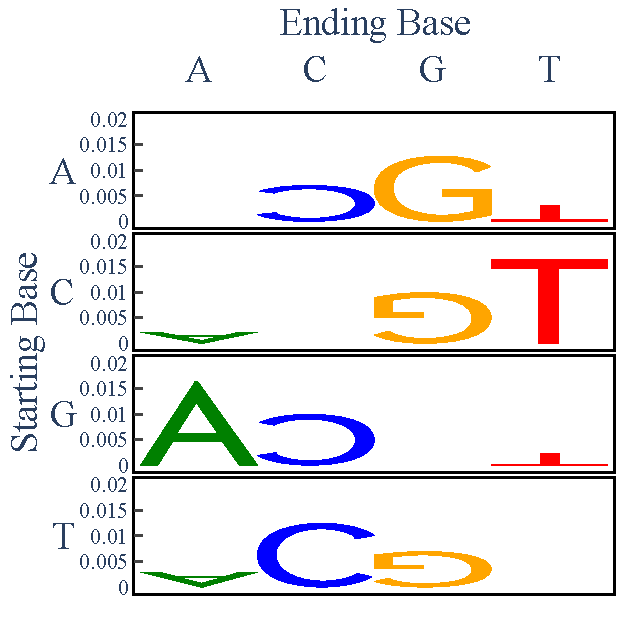
\includegraphics[scale=0.7]{graphics/spectra_Panc-AdenoCA.pdf}
    \caption{Panc-AdenoCA}
    \label{fig:spectra_panc_adenoca}
    \end{subfigure} \\
    \vspace{0.2cm}
    \caption{\textbf{Base substitutions are a rich source of information}. Here, $RE$'s as a measure of information are shown in mutation logos for (a) Skin-Melanoma (b) Kidney-RCC (c) Liver-HCC (d) Panc-AdenoCA. The other cancers can be found in Figure \ref{fig:apdx_spectra}. For each panel, each row was derived from a pair of GLMs corresponding to a wildtype base. The x-axis is the wildtype base; the y-axis is the product of the substitution. The heights of the letters are $RE$'s. An up-orientation indicates an excess while a down-orientation indicates a deficit of the mutation.}
    \label{fig:spectra}
\end{figure}

\section{Information available in flanking bases}

\part{Results: Building the classifier}{
    Based on the finding presented in chapter \ref{gle} and \ref{sce}, the following chapter will present the classifier (\gls{classifier}) built on \gls{gle} and \gls{sce}. Briefly, this part trials different distance measures to estimate the dissimilarity between each pair of individual donors. Accordingly, this part also trials different ML algorithms that directly rely on pairwise distance/similarity measures like the \gls{knn} and the \gls{svm}. The accuracy of each approach, reported as \glspl{confusion matrix}, reveals interesting characteristics of cancer mutation data.  
}

\chapter{Classification}\label{ml}

Previously, Chapters \ref{gle} and \ref{sce} demonstrate that both \gls{gle} and \gls{sce} contributed to characterising the cancer mutagenesis patterns. Chapter \ref{gle} shows that the smooth representation of GLE was better at discriminating cancers than the bin representation. Chapter \ref{sce} shows evidence that there is an informational advantage in exploiting the bases beyond 3-mers, namely flanking positions -2 and +2 with respect to the substitutions. 

Nonetheless, to manipulate the information from GLE and SCE, they have to be represented correctly. A sensible instinct is that a more suitable representation of a feature gives higher accuracy than a less suitable representation. This chapter acts as both an application and a validation for chapters \ref{gle} and \ref{sce}. In particular, section \ref{ml:gle} shows that smoothing GLE is a better representation than binning it. Section \ref{ml:sce} shows that currently strand symmetric 3-mer is the preferable representation of SCE. Additionally, section \ref{ml:both} demonstrates we can combine two factors with different units, like GLE and SCE, in a joint model in an attempt to further improve accuracy and to weigh the importance of each in the presence of the other.

While each of the next sections works on different data inputs, all sections follow the same procedure for training the classifier (Methods \ref{methods:ml_workflow}). Briefly, a small proportion of data is set aside as a test set, which is then used to evaluate model performance.

\section{Classifiers based on GLE}\label{ml:gle}
This section seeks to identify the best approach to extract information from GLE for cancer prediction. Specifically, similar to section \ref{gle:bootstrap} of Chapter \ref{gle}, I trialled the bin \textit{v.s.} smooth representations together with the Euclidean \textit{v.s.} Wasserstein distances. Again, the conventional bin representation counts mutations in discrete segments of the genome while the smooth representation computes the density of genomic locations based on how dense mutations are distributed in the neighbourhood. The Euclidean distance between two vectors aggregates the differences between points at the same coordinates on the vectors while the Wasserstein distance allows comparing points at different coordinates. More detailed comparisons between the two representations and distance measures can be found in Methods \ref{methods:bootstrap}. For each representation and distance, I trained a KNN classifier with 1/10 of the donors being used as the test set. Comparing the observations in the test set to the predictions made by the classifier allowed calculating the accuracy measure $F1$. I iterated the training procedures 10 times to estimate the range of the $F1$ scores obtained from these approaches. $F1$ was chosen as the accuracy measure as it takes into consideration both sensitivity and specificity. Details about the training procedures can be found in Methods \ref{methods:ml_workflow}.

The results are summarised in Figure \ref{fig:f1_gle}. For the Euclidean distance, the smooth representation was much better than the bin approach in predicting cancers. This is also very clear when inspecting the confusion matrices (Figure \ref{fig:confusion_bin_euclidean} \textit{v.s.} \ref{fig:confusion_smooth_euclidean}), where many more observations lay on the diagonals for the smooth representation compared to the bin representation. This is consistent with the bootstrap results from section \ref{gle:bootstrap}, where the difference in GLE between cancers was more significant for the smooth representation than the bin representation. For the Wasserstein distance, the difference between the smooth and bin approach was not obvious (Figure \ref{fig:f1_gle} and \ref{fig:apdx_ml_gle}). Besides, the $F1$ scores for both representations with the Wasserstein distance were about the same as that for the smooth representation with the Euclidean distance. This suggests that the properties of the Wasserstein distance allows it to alleviate the pitfalls introduced by the bin representation, which will be discussed in details in Section \ref{} of Chapter \ref{discussion}. 

\begin{figure}[htbp]
    \begin{subfigure}{.5\textwidth}
    \centering
    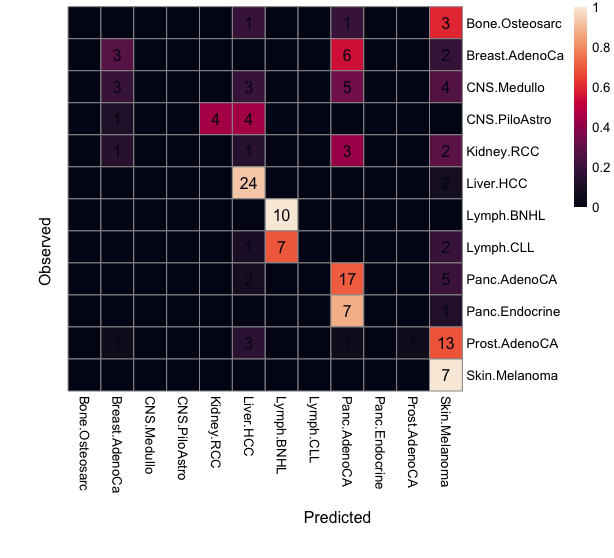
\includegraphics[width=\textwidth,height=0.9\textwidth]{graphics/confusion_matrix_bins_euclidean.png}
    \caption{Bin/Euclidean}
    \label{fig:confusion_bin_euclidean}
    \end{subfigure}
    ~
    \begin{subfigure}{.5\textwidth}
    \centering
    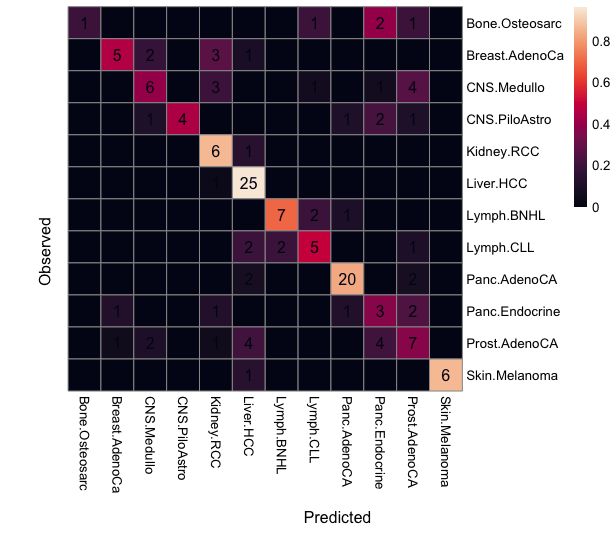
\includegraphics[width=\textwidth,height=0.9\textwidth]{graphics/confusion_matrix_smooth_euclidean.png}
    \caption{Smoothing/Euclidean}
    \label{fig:confusion_smooth_euclidean}
    \end{subfigure} \\
    \vspace{0.5cm}
    
    \begin{subfigure}{0.5\textwidth}
    \centering
    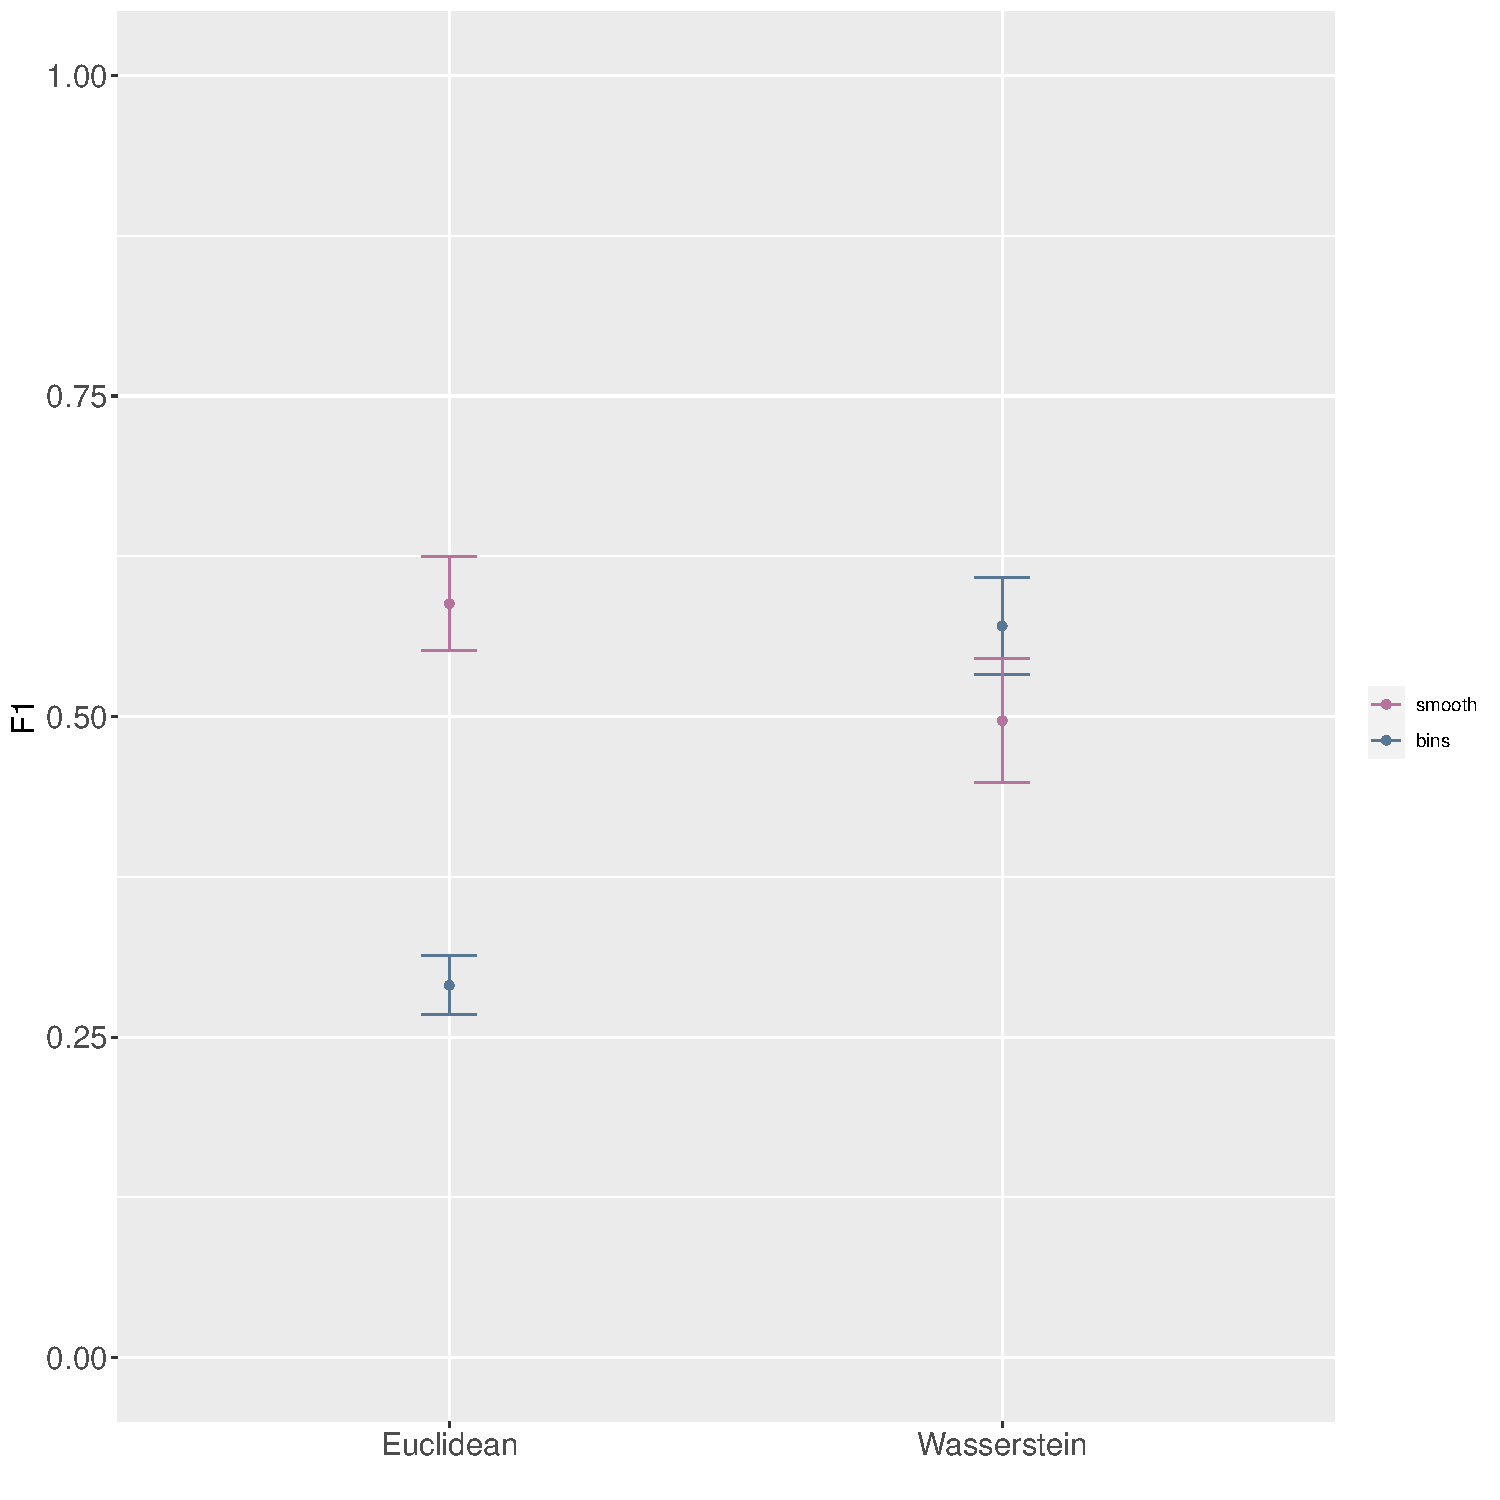
\includegraphics[scale=0.8]{graphics/f1_gle.pdf}
    \caption{F1 summary}
    \label{fig:f1_gle}
    \end{subfigure}
    
    
    \caption{\textbf{Smoothing was more accurate than binning for Euclidean distance, the difference between two representations was unclear for Wasserstein}. For each combination of representation/metric, I iterated the training procedures 10 times. Here, a representative confusion matrix, coloured by the percentage of predicted values over row total, is shown for (a) Bin/Euclidean, (b) Smooth/Euclidean. (c) shows the means of $F1$ for all representations/measures, the error bars are the standard errors for the iterated $F1$'s.}
    \label{fig:ml_gle}
\end{figure}

\section{Classifiers based on SCE}\label{ml:sce}

\subsection{3-mer was the most accurate sequence context size}
To train a classifier based on SCE, I experimented with incorporating the flanking bases to the mutation composition, including the context sizes of 1-mer, 3-mer and 5-mer, where 1-mer is the base substitution without any context. For each donor, the vector used to represent SCE was simply the counts of mutations with flanking bases incorporated divided by the total number of mutations. The detailed representation is described in Methods \ref{methods:ml_sce}, summarised in Figure \ref{}. In parallel, due to the strand symmetry observed in Chapter \ref{sce}, I also trialled imposing different levels of symmetry to SCE. These include asymmetry (no symmetry, \textit{i.e.} the normal count vector), semi-symmetry (reverse complementary base substitutions being counted as the same category) and full-symmetry (reverse complementary base substitutions being counted as the same category and flanking bases restricted to be A and C). Out of three levels of symmetry, the semi-symmetric representation was the commonly used method that was introduced in Section \ref{intro:sce}; the fully-symmetric representation was an experiment with the length of the SCE vectors. Methods \ref{methods:ml_sce} and Figure \ref{} provide a more detailed depiction of the representations for the three levels of strand symmetry. The algorithm and the accuracy measure recruited for SCE were KNN and $F1$, respectively, with Jensen-Shannon used as the distance measure. 

Figure \ref{fig:f1_sce} shows the $F1$ for different $k$-mer sizes and different levels of strand symmetry. The corresponding confusion matrices can be found in Figure \ref{}. In general, SCE was more accurate than GLE, with 3-mer being the best representation ($F1=0.78$). Asymmetry and semi-symmetry performed roughly similarly, reinforcing the evidence of strand symmetry previously seen in Chapter \ref{sce}. Assuming asymmetry and semi-symmetry are equivalent, $F1$ being lower for 5-mer than 3-mer but higher for semi-symmetry than asymmetry is very curious. Combined with the observation in section \ref{sce:nbr} of Chapter \ref{sce} that there was information in the outer positions -2 ans +2, this suggests there is an impact of splitting up mutation counts into too many elements in 5-mers (Table \ref{tab:sce_symmetric}). However, the length of the input vector was not the only determinant of accuracy as the fully symmetric representation, despite its short vector, severely dropped in accuracy. This suggests that the fully symmetric representation introduced noise to the data.

\begin{figure}[h!]
    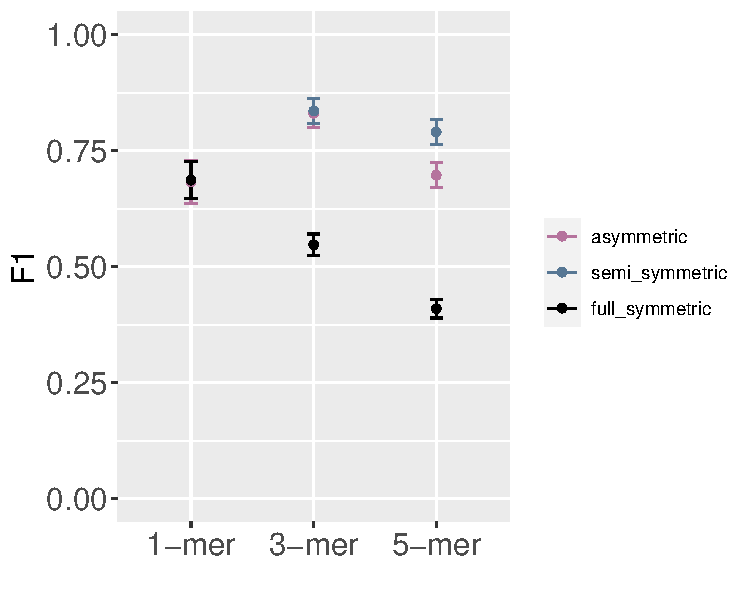
\includegraphics[scale=0.75]{graphics/f1_sce.pdf}
    \caption{\textbf{SCE classifiers using the 3-mer context  were the most accurate}. For each combination of representation/metric, I iterated the training procedures of the KNN classifier 10 times using Jensen-Shannon distance. The performance of the classifier was computed based on a previously held out test data set and reported as confusion matrices and $F1$'s. The y-axis is the means of $F1$ for 1-mer, 3-mer \& 5-mer and asymmetry, semi-symmetry \& full-symmetry; the error bars are the standard errors for the iterated $F1$’s. The corresponding confusion matrices are shown in Figure \ref{fig:apdx_ml_sce}.}
    \label{fig:f1_sce}
\end{figure}


\subsection{Dissecting 5-mer into submotifs could potentially improve accuracy}
Suspecting that the poor performance of 5-mer was due to the long vector that represented it, I tried splitting up 5-mers into smaller vectors that incorporate fewer flanking positions. To demonstrate, for 2-submotifs, I split the long 5-mer vector into 4 shorter vectors that only involved 2 positions, the base substitution and one flanking position. Similarly, 3-submotifs are 3 short vectors, each involving the base substitution and two flanking positions. The component short vectors provided pairwise distance matrices, which were averaged to make a final distance matrix as input to the KNN classifier. This is described in details in Methods \ref{methods:ml_sce}. The subsequent steps were the same as the normal training procedures.

Figure \ref{fig:f1_sce_submotif} shows that the splitting did improve $F1$ compared to the original whole 5-mer vector, particularly the 3-submotif representation. The corresponding confusion matrices can be found in Figure \ref{}. This is very promising, but at this point it is uncertain whether it was the information from outer flanking positions or the 3-mer incorporated in the 3-motifs that drove this accuracy improvement.

\begin{figure}[h!]
    \centering
    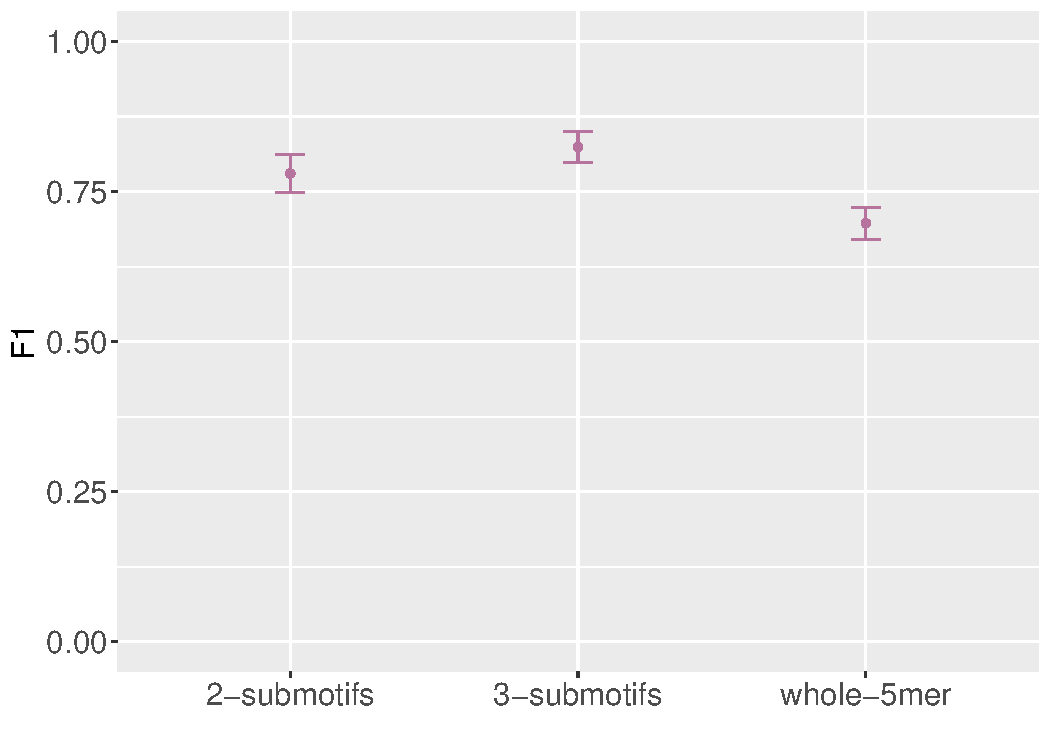
\includegraphics[scale=1]{graphics/f1_sce_submotif.pdf}
    \caption{\textbf{Dissecting 5-mer into multiple submotifs can potentially improve prediction accuracy compared to whole 5-mer}. For each combination of representation, I iterated the training procedures 10 times. The y-axis is the means of $F1$ for all representations/measures, the error bars are the standard errors for the iterated $F1$'s.}
    \label{fig:f1_sce_submotif}
\end{figure}


\section{Classifiers based on the combination of GLE and SCE}\label{ml:both}
In this section, I attempted to combine GLE and SCE to see whether the combination could improve the accuracy over each factor by itself. In terms of representation, I used two approaches, the conventional and the proposed approach. The conventional approach combined the bin representation for GLE and the semi-symmetric 3-mer representation for SCE. The proposed approach combined the smooth representation for GLE and the asymmetric 3-mer representation for SCE. For both approaches, I used the Euclidean distance for GLE and Jensen-Shannon distance for SCE. To combine GLE and SCE, I converted the distance matrices for the two factors into the kernel matrices, during which their scales and units were normalised. I then combined the kernel matrices, trialling different weights and converted the resulting kernel matrix into a joint distance matrix (details in Methods \ref{methods:ml_both}). The subsequent steps were the same as the normal training procedures.

I reported $F1$ in Figure \ref{fig:f1_combined} and the corresponding confusion matrices in Figure \ref{}. For both approaches, $F1$ improved for GLE but not SCE. In fact, the accuracy was predominated by SCE, which is particularly true for the bin/semi-symmetry combination. Since both GLE and SCE were previously normalised, the influence of SCE on $F1$ shows that it was the stronger predictor of cancers than GLE.

\begin{figure}[h!]
    \centering
    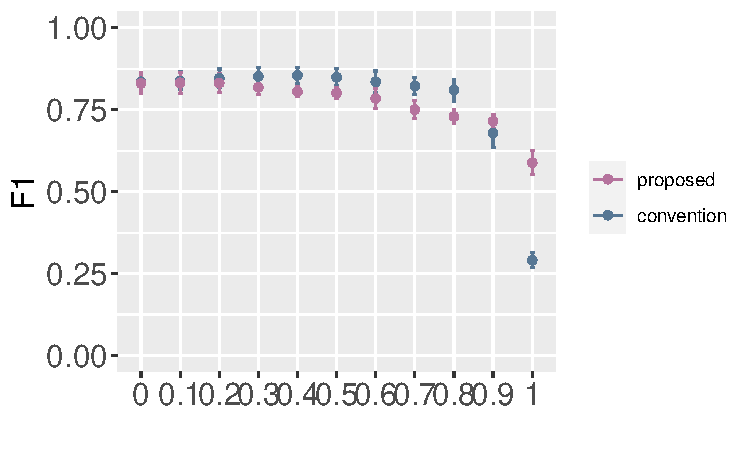
\includegraphics[scale=0.7]{graphics/f1_combined.pdf}
    \caption{\textbf{SCE was the stronger predictor of cancer prediction}. I combined GLE and SCE using two approaches: the conventional approach (bin for GLE and semi-symmetric 3-mer for SCE) and the proposed approach (smooth for GLE and asymmetric 3-mer for SCE). I used Euclidean distance for GLE and Jensen-Shannon distance for SCE. The x-axis is the weight given to GLE $g$, the weight given to SCE is accordingly $1-g$. For each weight combination, I iterated the training procedures 10 times. The y-axis is the means of $F1$ for all representations, the error bars are the standard errors for the iterated $F1$'s.}
    \label{fig:f1_combined}
\end{figure}


\section{Chapter summary}
In accordance with Chapters \ref{gle} and \ref{sce}, this chapter shows that both GLE and SCE are good predictors of cancers, with SCE being the stronger factor. All classifiers used the KNN algorithm with $F1$ as the measure of accuracy. Section \ref{ml:gle} shows that the smooth representation of GLE was more accurate than the bin representation. However, the Wasserstein distance had properties that allowed it to alleviate the pitfalls from the bin representation. Section \ref{ml:sce} shows that the information from flanking bases were useful for cancer classification, using the Jensen-Shannon distance. In particular, the 3-mer representation with three positions involved, the base substitution and positions -1 and +1, performed best. That said, the length of the SCE vector had an impact on the performance of the classifier. This manifests in that 5-mer was less accurate than 3-mer, even though information was shown to be available in positions -2 and +2 in Chapter \ref{sce}. Besides, the accuracy for 5-mer improved when splitting it up into shorter vectors. Evidence of strand-symmetry was again present, as the semi-symmetric representation was at least as accurate as the asymmetric representation. Finally, Section \ref{ml:both} shows that SCE was the stronger predictor of cancers than GLE, because the accuracy was mostly determined by SCE even after both GLE and SCE were normalised.


\chapter{Conclusion and Discussion}\label{discussion}

This project has shown that both mutation location in the genome and the composition of mutations were important characteristics of the cancer mutation profile. Regarding the genomic location effect (GLE), mutations were shown to preferably occur in closed chromatin regions over open chromatin regions. GLE helped characterise the mutation profile because it differed significantly between cancers. More importantly, the smooth representation was better at extracting information from GLE than the bin representation for cancer classification (Chapter \ref{gle}). Regarding the sequence context (SCE) for mutation composition, this project has shown that SCE contributes a considerable amount of information to the cancer mutation profile. Cancers had very different composition of mutations and the difference came from both the base substitutions and the flanking bases. Mutation composition was strand-symmetric and there was more information from transitions than there was from transversions (Chapter \ref{sce}). The project also developed a mutation-based classifier of cancer using the distance-based algorithm KNN. In general, I found that both GLE and SCE were shown to be predictive of cancers, SCE was the dominating predictor (Chapter \ref{ml}).

\section{Genomic location effect}
\subsection{Speculation of the mechanisms driving GLE}
My conclusion that mutations tend to occur in closed regions agree with previous observations \citep{Polak2015,Fujimoto2016Whole-genomeCancer,Prendergast2007ChromatinGenome}. Notably, \citet{Polak2015} used different measures of chromatin structure, including DHS and histone marks such as H3K4me1, to predict mutation density in Mbp bins. While the $OR$ mislabelling experiment of this project found that chromatin structure of the original cells was influential on GLE but unlikely to determine whether GLE differed between cancers (Section \ref{gle:mixed_or}), \citet{Polak2015} showed that chromatin structure data from correct cell types of origin were more correlated with the mutation density of the cancer than mislabelled cell types. The two results were not directly compatible, as the difference might have come from the different set of cancers investigated and the different types of data representing chromatin status (explained below). However, looking at the reported variance explained $R^2$ from \citet{Polak2015}, their claim was only really convincing for skin melanoma (Skin-Melanoma) and hepatocellular carcinoma (Liver-HCC), which are two distinctive cancers even in my project. 

Several factors could potentially interfere with the reliability of the DHS data recruited to represent chromatin status. First, for simplicity, I used the binary representation of DHS that treats genomic regions as either open or closed regions. However, the accessibility of DNA is actually more complicated, as there is variation in the openness of open chromatin regions \citep{Boyle2008High-ResolutionGenome}. A continuous representation instead of the binary representation used in this project would therefore be more accurate. Second, there was a degree of uncertainty in the identification of the cells of origin. This is particularly true for medulloblastoma (CNS-Medullo), whose cell types of origin is still just a speculation \citep{Penas2015TheMedulloblastoma} but less true in skin melanoma, whose original cell type is quite established to be melanocyte \citep{Lin2007MelanocytePigmentation}. Besides, each DHS data for a cell type provided by ENCODE came from just one individual \citep{Thurman2012TheGenome}. Third, chromatin structure could be modified during carcinogenesis, for example due to mutations in chromatin modifier genes \citep{Makova2015TheGenome}. While this is an identified problem, there is no easy way to account for this given the availability of accessible data that I am aware of. I expect that using DHS data for the cancer itself rather than its original cell type is unlikely the solution because the modifications in chromatin structure differ between samples of similar cancer type across different stages of cancer.

Assuming DHS data is reliable, I hypothesise another explanation for the ability of GLE to predict cancers: the interaction between chromatin structure and the distribution of base compositions across the genome rather than the chromatin structure itself. This is explained in Figure \ref{fig:discussion_gle}. Essentially, I hypothesise that some genomic regions have higher mutation density not only because they are in the closed chromatin but also because they contain bases that are prone to be targeted by a specific mutagen. Given that chromatin structure affects GLE, this explanation will make sense if the variation in chromatin structure is not great enough to shape the diversity of GLE \textit{per se}. Indeed, \citet{Gilbert2004ChromatinFibers} showed that open chromatin regions contain gene clusters, hypothetically for expression and protection of genes \citep{Gilbert2004ChromatinFibers,Gazave2005DoesDamage}. This suggests a certain degree of conservativeness in chromatin structure as genes universal to all cell types will be more likely located in open chromatin regions. My proposed explanation can be evaluated by examining the association between the types of substitutions (whether the wildtype is A/T or C/G) and their location (whether they locate in closed or open chromatin regions) as well the association between the cancer type (whether mutations with wildtype A/T are from cancer A or B) and their genomic location with respect to the cancers (closed or open regions). 

\begin{figure}[h!]
  \begin{minipage}[c]{\textwidth}
    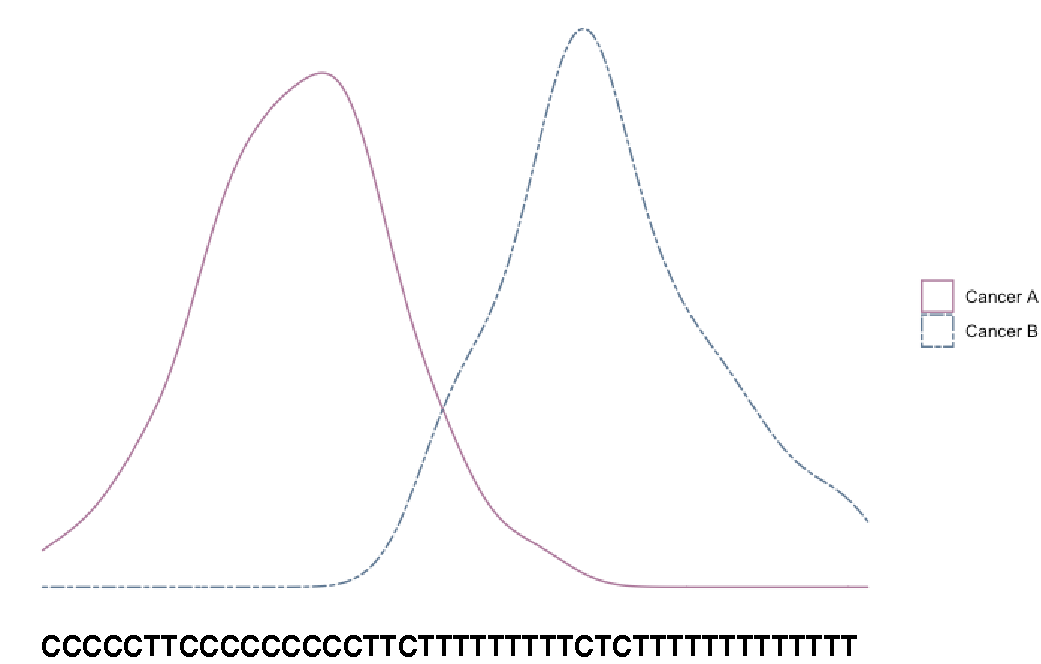
\includegraphics[scale=0.9]{graphics/discussion_gle.pdf}
  \end{minipage}\hfill
  \vspace{1cm}
  
  \begin{minipage}[c]{0.48\textwidth}
  \centering
    \begin{tabulary}{\columnwidth}{rRR}
    \toprule
        & \textbf{A/T mutated (Cancer A)} &  \textbf{C/G mutated (Cancer A)} \\
    \hline
        \textbf{closed} &  &   \\
        \textbf{open} &  &   \\
    \bottomrule
    \end{tabulary}
  \end{minipage}\hfill
  \begin{minipage}[c]{0.48\textwidth}
    \begin{tabulary}{\columnwidth}{rRR}
    \toprule
        & \textbf{A/T mutated (Cancer A)} &  \textbf{A/T mutated (Cancer B)} \\
    \hline
        \textbf{closed} &  &   \\
        \textbf{open} &  &   \\
    \bottomrule
    \end{tabulary}
  \end{minipage}
  \vspace{0.5cm}
  
  \begin{minipage}[c]{\textwidth}
    \caption{
      \textbf{Proposed explanation for why GLE differ between Cancer A and Cancer B.} Cancer A is under the influence of a mutagen that targets the base C; Cancer B is under the influence of a mutagen that targets the base T. Some regions of the genome are more enriched in C, other are enriched in T. The distribution of bases combines with chromatin structure to influence GLE. This could be evaluated by assessing whether certain substitutions are enriched in closed/open chromatin regions, or whether two cancers differ in how mutations with wildtype A/T are distributed between closed/open chromatin regions.
    } \label{fig:discussion_gle}
  \end{minipage}
\end{figure}


\subsection{Representing GLE}
In this work, I showed that the smooth representation of GLE was better than the bin representation for both the bootstrap hypothesis testing (Section \ref{gle:bootstrap}) and the GLE-based classification (Section \ref{ml:gle}). For the bootstrap study, the p-value was not necessarily contrasted against a significance threshold, but it really was an indication of the ``extremity'' of the observed distance between cancers against the null. Interestingly, the Wasserstein distance somehow redeemed the performance of the bin representation compared to the smooth representation. As previously mentioned (Figure \ref{fig:mutdistribution_demo} of Section \ref{intro:gle}), the drawback of the bin representation is that it imposes arbitrary rigid boundaries to the genome. However, looking at its definition (Methods Figure \ref{fig:wasserstein_demo}), the Wasserstein allows comparisons of bins with different coordinates, thereby ``breaking'' the rigid boundaries. In other words, the Wasserstein distance itself has a smoothing effect. Regarding the 1 Mbp bin size, \citet{Hodgkinson2012TheGenomes} stated that the variation in GLE was detected at the 1 Mbp scale, but blurred out at 10 Mbp scale. Although the two scales are quite different, and the Mbp scale was not demonstrated to be the lower limit, this established that the use of 1 Mbp was reasonable. Accordingly, the choice of using the smooth representation or the bin representation combined with Wasserstein distance should therefore depend on computing performance. 

\section{Sequence context effect}
\subsection{Patterns of mutation composition}
Using the measure of information $RE$, I detected patterns of mutation composition that were compatible with previous work \citep[Chapter \ref{sce};][]{Alexandrov2020}. In particular, \citet{Alexandrov2020} decomposed the composition of mutations using non-negative matrix factorisation to identify the so-called ``mutation signatures''. They established that signature SBS7a, presumably associated with UV exposure, was found in all skin melanoma samples and was only found in skin melanoma. This signature is predominated by the C$\rightarrow$T substitution, especially when there is a T at flanking position -1. This is consistent with my observation in Figures \ref{fig:spectra_skin} and \ref{fig:transitions_skin}. Likewise, signature SBS12 detected only in hepatocellular carcinoma was enriched in the T$\rightarrow$C substitution, which is in line with the observation in Figure \ref{fig:spectra_liver}. The work of \citet{Alexandrov2020} is a detailed decomposition of mutation compositions, where each cancer can have multiple signatures. In the meantime, my work, developed on top of \citet{Zhu2017}, was analogical to a general summary of mutation composition. 

\subsection{Strand symmetry}
Both $RE$ (Chapter \ref{sce}) and the SCE-based classifier (Section \ref{ml:sce}) of my project showed evidence of strand symmetry, in the sense that reverse complementary mutations are counted as the same category (introduced in Figure \ref{fig:motif_symmetric_demo} of Section \ref{intro:sce}). This representation, which I referred to as semi-symmetry, was adopted by most publication that I am aware of \citep{Alexandrov2020,Jiao2020,Zhang2020}. However, \citet{Zhu2017} showed that the compositions of flanking bases to a substitution significantly differed between two DNA strands in skin melanoma. This is not necessarily contradictory with my finding, but it reflects the fact that the data I used did not specify what mutations occurred on which DNA strand. Nevertheless, this shows that given this type of data, which is often the case, the semi-symmetry representation should be sufficient to capture information.

\subsection{Flanking bases beyond 3-mers}
There was inconsistency in the $RE$ of flanking positions (Section \ref{sce:nbr}) and the SCE-based classifier (Section \ref{ml:sce}) with respect to the importance of bases at positions -2 and +2. Even though information was observed in these positions using $RE$, incorporating them into the classifier (5-mer) led to a drop in accuracy. I attributed this to the size of the vector representing 5-mers. Both the attempt to break the 5-mer vector down into shorter vectors and the introduction of semi-symmetry improved accuracy for 5-mers, which supports my speculation. It is worth noting that the fully symmetric representation decreased accuracy instead of improving it. This representation was an attempt to shorten the SCE vector without a biological basis; therefore, its results indicate that the length of the representation vector was not a determinant of accuracy without a good biological rationale. In comparison with the literature, \citet{Zhu2020} showed that it was possible to identify the origin of a single mutation based on its flanking bases. \citep{Zhang2020} showed that using the sequence context of the 9-mer context was the best at predicting cancers, both for simulated data and for breast cancer subtypes. Their results were obtained using the support vector machines, which is a kernel based classifier algorithm. As described in Methods \ref{methods:ml_both}, one way to compute pairwise kernel matrices is via pairwise distance matrices.  This is a great support for the potential of incorporating bases beyond 3-mers. However, while \citet{Zhang2020} also split up large context sizes, their representation forced bases of the same distance to the substitution (\textit{e.g.} positions -1 and +1) to have the same weight. As previously seen from Figure \ref{sce:nbr}, for a mutation (\textit{e.g.} C$\rightarrow$T), the contribution of position +1 to the information context was different from that of position -1.

\section{Misclassification and improvement of accuracy}
\subsection{Common patterns of misclassification}
Some patterns of misclassification can be observed for the GLE-based classifiers, but there was no obvious patterns for the SCE-based classifiers. Prior to the project, I had expected the GLE-based classifiers to misclassify epigenetically similar cancers due to the influence of chromatin structures on GLE. However, it is important to notice that epigenetically similar cells are also likely to be under the influence of chemically similar environments (\textit{e.g.} similar mutagens). This expectation was true for the two lymphocyte related cancers, chronic lymphocytic leukaemia (Lymph-CLL) and B-cell non-Hodgkin's lymphoma for all representations and distance measures (Figures \ref{fig:confusion_smooth_euclidean}, \ref{fig:confusion_bin_euclidean} and \ref{fig:apdx_ml_gle}). From the the multidimensional scaling plot (Figure \ref{fig:encode_pca}), which groups epigenetically similar cell types together, because Skin-Melanoma and Liver-HCC were far away from other cancers, they were expected to be distinctive cancers. This was generally the case, with the exception of the bin representation using the Euclidean distance. Almost all donors with Skin-Melanoma and Liver-HCC were correctly identified, and donors predicted to have these cancers really did. From Figure \ref{fig:encode_pca}, we would expect prostate adenocarcinoma (Prost-AdenoCA) and pancreatic adenocarcinoma to be misclassified because they seemed very similar in terms of chromatin structure. This expectation was only partly met when using the Wasserstein distance (Figure \ref{fig:apdx_ml_gle}). Regarding the SCE-based classifiers, the misclassified cancers were not consistent between different representations. One vague pattern was that CNS-Medullo was sometimes mistaken for Prost-AdenoCA (for the 3-mer and the submotif classifiers, Figures \ref{fig:confusion_3mer}, \ref{fig:confusion_3mer_symmetric}, \ref{fig:confusion_2-submotifs} and \ref{fig:confusion_3-submotifs}). At this point, it is uncertain whether this suggests some interesting common patterns of mutation compositions between the two cancers or just an artefact. 

In comparison with the previous study by \citet{Jiao2020}, it was also found that misclassification was common between Lymph-CLL and Lymph-BNHL and between the brain cancers CNS-Medullo and pilocytic astrocytoma (CNS-PiloAstro). The former was consistent but the latter was not observed for our project. \citet{Jiao2020} attributed the misclassification patterns to the similarity in the epigenetics of the cancers. Based on my analysis of the chromatin structure, I only partly agree with this speculation. I propose that chromatin structure has some contribution to the misclassification but there are other parallel factors involved. An example of such factors is illustrated in Figure \ref{fig:discussion_gle}.

\subsection{Classification accuracy}
The best performing classifier for GLE was the smooth representation using Euclidean distance (mean $F1=0.59$; Section \ref{ml:gle}); the best performing classifier for SCE was the 3-mer representation (mean $F1=0.83$; Section \ref{ml:sce}). Combining GLE and SCE did not improve accuracy, but the accuracy was mostly determined by SCE (Section \ref{ml:both}). \citet{Jiao2020} also attempted to develop classifiers of cancers based on mutation data. Using the Random Forest (RF) classifier algorithm \citep{Lindner2017AutomatedModels}, they found that the classifiers by either GLE or SCE individually produced $F1\approx0.7$. Their attempt to combine GLE, SCE and other factors (such as the genomic distribution of copy number variations or structural variation) resulted in a median $F1=0.86$. Because GLE and SCE were the best predictors in their examined predictors, it can be assumed that $F1=0.86$ was mostly contributed by the two factors. The improvement of accuracy when combining GLE and SCE over the individual classifier in the case of \citet{Jiao2020} might be because their individual classifiers were compatible with respect to accuracy. In the meantime, the level of accuracy for the combined classifier in our case only depended on SCE, but our SCE-based classifier was much more accurate than the GLE-based classifier in the first place. 

\subsubsection{Improving accuracy by data representations}
There are several tweaks to the representation of both GLE and SCE that could potentially improve accuracy over the models developed during my project. For GLE, I have computed the distances between donors by summing up the distances for all chromosomes. Knowing that chromosomes vary in lengths, we could trial weighing different chromosomes according to their lengths. For SCE, because the evidence supporting the usefulness of flanking bases beyond 3-mers was plenty, including the measure of information in Section \ref{sce:nbr} and the results reported by \citet{Zhang2020}, further effort should focus on incorporating larger $k$-mer sizes. We have seen that information was available in positions -2 and +2, but less than in positions -1 and +1 (Section \ref{sce:nbr}). In this project, I gave all flanking positions the same weights. In future project, we could experiment with imposing weights on different components of the submotif representation for SCE. Finally, based on the speculation in Figure \ref{fig:discussion_gle}, it is also worth considering a way to represent the interaction between GLE and SCE. This could be in the form of an interaction term between the two factors, or a single factor that simultaneously accounts for both factors.

\subsubsection{Addressing imbalanced data}
One issue that has not been addressed in my project and \citet{Jiao2020} is the imbalanced data for classification. In my project, some cancers had more than 200 donors (\textit{e.g.} Liver-HCC) and some only had fewer than 80 donors (\textit{e.g.} bone osteosarcoma, Bone-Osteosarc). This could lead to biased predictions, described in Figure \ref{fig:imbalanced}, in which new observations of the minor class are misclassified as the major class because there are not enough data points supporting the minor in the training set. For my project, this was most obvious in Bone-Osteosarc (44 donors), which tended to be identified as another cancer in a seemingly random manner. Established methods to address the issue of imbalanced classification worth taken into consideration include under-sampling and over-sampling. Both methods attempt to make the number of data points roughly similar between the major and the minor class. Under-sampling involved excluding data from the major class and keeping the number of data points from the minor class, which is quite straightforward \citep{Kubat1997AddressingSelection}. Over-sampling involved simulating more data from the minor class and keeping the number of data points from the major class \citep{Chawla2002SMOTE:Technique}. The over-sampling simulation introduced by \citet{Chawla2002SMOTE:Technique} is a distance-based algorithm that creates new observations that are closer to the minor class than the major class. 

\begin{figure}[ht!]
    \centering
    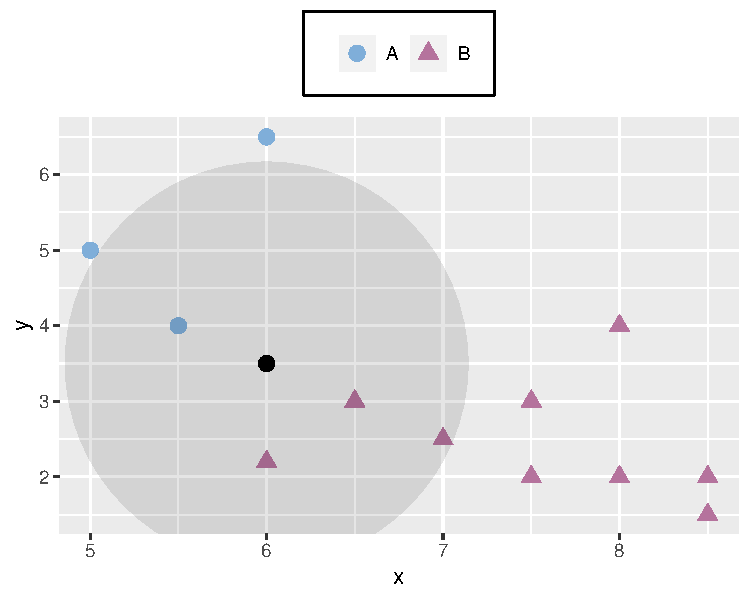
\includegraphics[scale=0.9]{graphics/imbalanced.pdf}
    \caption{\textbf{Impact of imbalanced design.} Cancer A (circle) is the minor cancer with fewer observations. Cancer B (triangle) is the major cancer with more observations. When a new data point representing Cancer A (black circle) is to be predicted, it tends to be misclassified as Cancer B because there is not enough confidence for the classifier to predict it to be Cancer A.}
    \label{fig:imbalanced}
\end{figure}


\subsubsection{Choosing the machine learning algorithms}
The choice of the machine learning algorithms could also affect accuracy. For example, when training a classifier combining GLE and SCE, \citet{Jiao2020} reported that the deep neural network (DNN) classifier was better than the RF classifier (DNN was not used to train GLE and SCE individually). Even though there are known strengths and drawbacks for each classifier \citep{Susmita2019AAlgorithms}, the performance can be very context dependent. In this project, I chose the KNN because it is convenient for my distance-based representation of data and because of its interpretability. By contrast, DNN is often thought of as a ``black box'' that is hard to understand and manipulate \citep{Shwartz-Ziv2017OpeningInformation}. However, in future work, it is worth experimenting with different algorithms and establishing which algorithms are suitable for mutation-based classifiers of cancers. 

\section{Cancer diagnosis and mutation based classifiers}
Cancer diagnosis is an important step in cancer management \citep{Tobias2014CancerManagement}. Early diagnosis is one of the keys to cancer treatment \citep{Hawkes2019CancerDiagnosis}. For this reason, several schemes for cancer screening have been employed to detect certain cancers in high risk individuals on a population scale \citep{Tobias2014CancerManagement}. For example, women aged 20-65 in the UK are encouraged to have a Papanicolaou test \citep{Bharadwaj2013HumanTreatment} for cervical cancers every three years \citep{Tobias2014CancerManagement}. It would be beneficial to be able to detect cancers systematically at an early stage. As mentioned in Section \ref{intro:significance}, with the development of liquid biopsy, it might be possible in the long term that we could predict what cancer is present based on circulating tumour DNA in the blood upon successful development of a mutation-based classifier. In terms of diagnosis, multiple evaluations are usually required to reach a conclusion \citep{Tobias2014CancerManagement,Stone1995Biopsy:Pitfalls}. Two important tools for cancer diagnosis are biopsy and immunohistochemistry (IHC), which require manual interpretation of trained pathologists \citep{Stone1995Biopsy:Pitfalls,Ahmed200615Cancer}. However, it can sometimes be challenging even for trained pathologists to correctly identify cancers from IHC without prior knowledge of other factors such as the patients' clinical history, particularly when given a \gls{metastasis} of unknown primary \citep{Sheahan1993MetastaticStatus,Rassy2020ExploringToday}.  

As a result, it is always desirable to have an additional diagnostic tool, particularly a quantitative one with explicit statistical confidence. Whilst there is a long way to go, my project is a demonstration of the feasibility of such a tool. The classifiers trained in this project were completely based on mutation data. Both aspects of the mutation examined were backed up by statistical analyses. The performance of the classifiers I developed was certainly better than random prediction (a rough estimation of the random threshold in this case is an accuracy score $<\frac{1}{12}$ because 12 cancers were analysed). If such a classifier is successfully developed in real life, it can act as either an exploratory evaluation or a validation tool for cancer diagnosis because it approaches the problem from a different perspective to a pathologist's. 

\section{Concluding remarks and summary of future directions}
\chapter{Methods}\label{methods}

For this project, I am interested in two factors that help characterise the cancer mutation profile: genomic location effect (GLE) and sequence context effect (SCE; Figure \ref{fig:workflow}). I examined each factor on two complementary scales: analysis of whole disease (section \ref{methods:gle} and \ref{methods:sce}) and cancer classification for individuals (section \ref{methods:ml}). The former was partly used to interrogate the biological basis for the latter, whereas the latter could validate the patterns detected by the former.

\begin{figure}[h!]
    \centering
    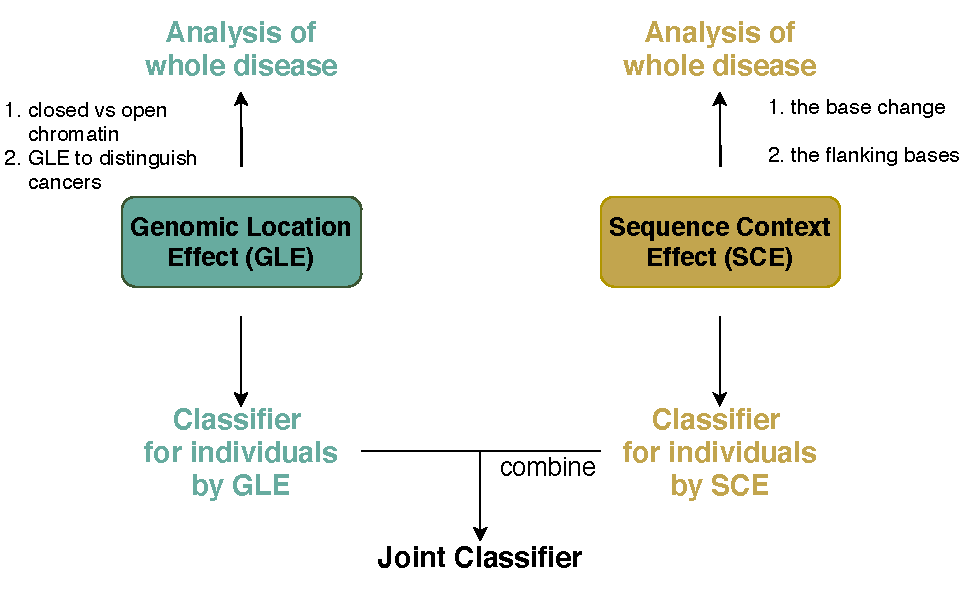
\includegraphics[scale=0.85]{graphics/workflow.pdf}
\caption{}
    % \caption{\textbf{Project workflow for understanding cancer mutagenesis data and exploiting it for cancer classification.} On one hand, cancers were analysed on the whole disease scale, which considered mutations from all donors of the same diseases as a whole. This magnified the signals in the data and made it easier for understanding the mutagenesis process. On the other hand, the information from the factors analysed above was used for training a classifier on the individual donor scale, meaning that this classifier could potentially be applied to a new patient's mutation data to predict their cancer. This followed a standard machine learning training procedure, outlined in Section \ref{methods:ml}.}
    \label{fig:workflow}
\end{figure}


\section{Data description}
\subsection{PCAWG - Mutation data} 
The critical source of data for the project was the mutation data provided by the Pan-Cancer Analysis of Whole Genome (PCAWG) project \citep{Campbell2020}. This data consisted of whole genome sequencing of both cancerous and healthy tissues (mostly blood) for all cancer patients, covering 2658 cancer samples from 28 cancer types. PCAWG relied on contrasting the cancerous against healthy tissues to determine whether a mutation was a \gls{sommut}. Mutations were identified by combining three established pipelines (Sanger \citep{Jones2016CgpCaVEManWrapper:Data}, EMBL/DKFZ \citep{Rimmer2014IntegratingApplications}, and Broad \citep{Cibulskis2013SensitiveSamples}).

This project was limited to analysing somatic \glspl{point_mut}. I sampled 12 cancers whose DHS data for the putative original cells was also available (Table \ref{tab:encode}). A summary of the mutations for the 12 cancers can be found in the appendix (Table \ref{tab:mutation_summary}, Figure \ref{fig:mutation_summary}). Mutation data for all individuals and all mutations was downloaded as a MAF file from the \href{https://dcc.icgc.org/releases/PCAWG/consensus_snv_indel}{International Cancer Genome Consortium (ICGC)}. Driver mutations were filtered out based on \href{https://dcc.icgc.org/releases/PCAWG/driver_mutations}{the PCAWG's driver mutation project} because driver mutations are under selection pressure and have different mutation rates to passenger mutations. Selection pressure was a confounder as the question of interest concerned the informativeness of the mutagenesis process. The information this project utilised from PCAWG was the mutations, their genomic locations, their donor ID and the donor's cancer. 

\subsection{Reference genome} 
To reconstruct the cancer genome, both mutation data and a standard human reference genome are required. The human reference genome was downloaded from the \href{http://hgdownload.soe.ucsc.edu/goldenPath/hg19/chromosomes}{UCSC genome browser}. As PCAWG used Human Genome Assembly 37, the same version of genomic coordinates was used for this project. As an additional check, I also established that the wildtype base at each mutated position and its local reference sequence context provided by PCAWG matched the sequence at that position from the reference genome. 

\subsection{DHS data for chromatin status} 
Part of my project investigated the relationship between mutation distribution and chromatin status. Based on literature search, I identified the most likely tissue of origin for the cancer of interest. These are summarised in Table \ref{tab:encode}. DNase I hypersensitivity (DHS) data for these tissues of origin, as a canonical measure for chromatin status, was from the ENCODE study \citep[downloaded from either \href{https://genome.ucsc.edu/cgi-bin/hgFileUi?db=hg19&g=wgEncodeOpenChromDnase}{Duke} or \href{https://genome.ucsc.edu/cgi-bin/hgFileUi?db=hg19&g=wgEncodeUwDnase}{UW};][]{Thurman2012TheGenome,Klemm2019ChromatinEpigenome}. Specifically, ENCODE measured the level of Dnase hypersensitivity across the genome and identified Dnase hypersensitive regions based on a threshold set by an established algorithm \citep{Boyle2008High-ResolutionGenome}. I used ENCODE identification of Dnase hypersensitive spatial ranges in the genome as open chromatin regions and the rest of the genome as closed chromatin regions.

\section{Algorithm development}\label{methods:code}
\subsection{Reproducibility} 
\href{http://git-scm.com}{Git} was used as a Version Control tool. Accordingly, the entire code history has been recorded and stored on \href{https://github.com}{GitHub}.

The entire project was done iteratively, which means that most analyses were repeated on increasing scales. This not only increased the opportunity for code efficiency to be improved but also helped ensure that the algorithms are reproducible. 

The code projects are available in the GitHub repositories \href{https://github.com/GavinHuttley/PhuongAnalysis}{PhuongAnalysis}, \href{{https://github.com/GavinHuttley/PhuongData}}{PhuongData}, \href{https://github.com/GavinHuttley/PhuongLibrary}{PhuongLib} and \href{https://github.com/Phuong-Le/PhuongR}{PhuongR}. All code is available upon request for now, but will be made public when more thorough testing is complete. 

\subsection{Developing packages}
Most core functions were written in Python v3.8.6 \citep{van1995python}, with visualisation and some analyses written in R v4.1.0 \citep{r}. Python libraries directly involved in data analysis were \texttt{numpy} v1.20.0 \citep{harris2020array}, \texttt{scipy} v1.6.0 \citep{2020SciPy-NMeth}, \texttt{sklearn} v0.24.2 \citep{scikit-learn}, \texttt{cogent3} v2021.5.7a \citep{pycogent3} and \texttt{MutationMotif} v0.3 \citep{Zhu2017}. R libraries directly involved in data analysis were base R \citep{RCoreTeam2019R:Computing}, \texttt{pheatmap} v1.0.12 \citep{pheatmap} and packages from the \texttt{tidyverse} collection such as \texttt{ggplot2} \citep{tidyverse}. Code was written as packages that can be installed and utilised by anyone.

All core functions were tested under explicit hypothetical scenarios for correctness before being applied. This process is called unit testing. Each of the analyses required multiple core functions. For each analysis, core functions were combined in one commmand line application \texttt{\href{https://click.palletsprojects.com/en/8.0.x/}{click}} that can be run either in a terminal or a Jupyter Notebook. The \href{https://github.com/HuttleyLab/scitrack}{Scitrack} Python package was applied to these commands so all code, and  data inputs and outputs of the commands were tracked and saved as log files.

\subsection{Parallelisation}
When analysing large data sets, some steps could be considerably time-consuming, particularly the initial data filtering step and the simulation steps. Therefore, for several steps, I have written scripts for code parallelisation based on the original command line functions. For example, for an analysis that executes the same processes multiple times on independent data objects, the objects were ``distributed'' across different computer cores instead of being processed sequentially on a single computer. Parallelisation was done using OpenMPI \citep{gabriel04:_open_mpi} and \texttt{mpi4py} \citep{Dalcin2011ParallelPython}. This was performed using resources provided by the National Computational Infrastructure Australia.


\section{Whole disease analysis of GLE}\label{methods:gle}

The variation in chromatin structures of different cell types is believed to shape where mutations occur in the genome, giving rise to the genomic location effects (\gls{gle}) that are characteristic of cancers \citep{Polak2015}. The methods in this section serve two purposes: to formally test the presumed biological connection between chromatin structure and mutation locations, and to weigh the importance of GLE as a characteristic of the cancer mutation profile irrespective of the its driving mechanism.  

\subsection{Visualising DHS by multi-dimensional scaling}\label{methods:encode_pca}
Before establishing the relationship between mutation location and chromatin structure, I examined whether and how the relevant original cells were related in terms of chromatin structure using DHS data. The rationale was that if chromatin structure was a true determinant of mutation location, then tissues that were epigenetically similar should have roughly similar patterns of GLE. Furthermore, such similarity might interfere with the informativeness of the GLE as a predictor of cancer when training the classifier.

For each pair of cell types, the intersections of their open chromatin regions were identified. The difference between the pair was then calculated as:

\begin{equation}
    d = 1 - \frac{2i}{o_1 + o_2}
\end{equation}

where $d$ is the difference/distance, $i$ is the total lengths of the genomic regions covered by the intersections, $o_1$ and $o_2$ are the length of the open chromatin regions. Essentially $d$ is the ``complement'' of the ratio between the intersection $i$ and the average length of the open regions $o_1$ and $o_2$. 

Once the distances for all possible pairs of cell types were obtained, I decomposed these distances into their relative coordinates by multi-dimensional scaling. This was done by the R function \texttt{cmdscale}. The coordinates for the 3 most informative dimensions are reported in Figure \ref{fig:encode_pca}, Subsection \ref{gle:pca} of Chapter \ref{gle}.

\subsection{Mutation location in relation to chromatin status}\label{methods:chromatin}
To establish the relationship between the mutation location of a cancer and the chromatin status of its original cell type, I sorted mutations into open and closed chromatin regions as per Figure \ref{fig:gle_workflow}. I then used (1) the G-test for whether we could reject the null that mutations occur without any preference for closed or open regions and (2) the odds ratio statistic to measure the bias towards closed regions.

\begin{figure}[h!]
    \centering
    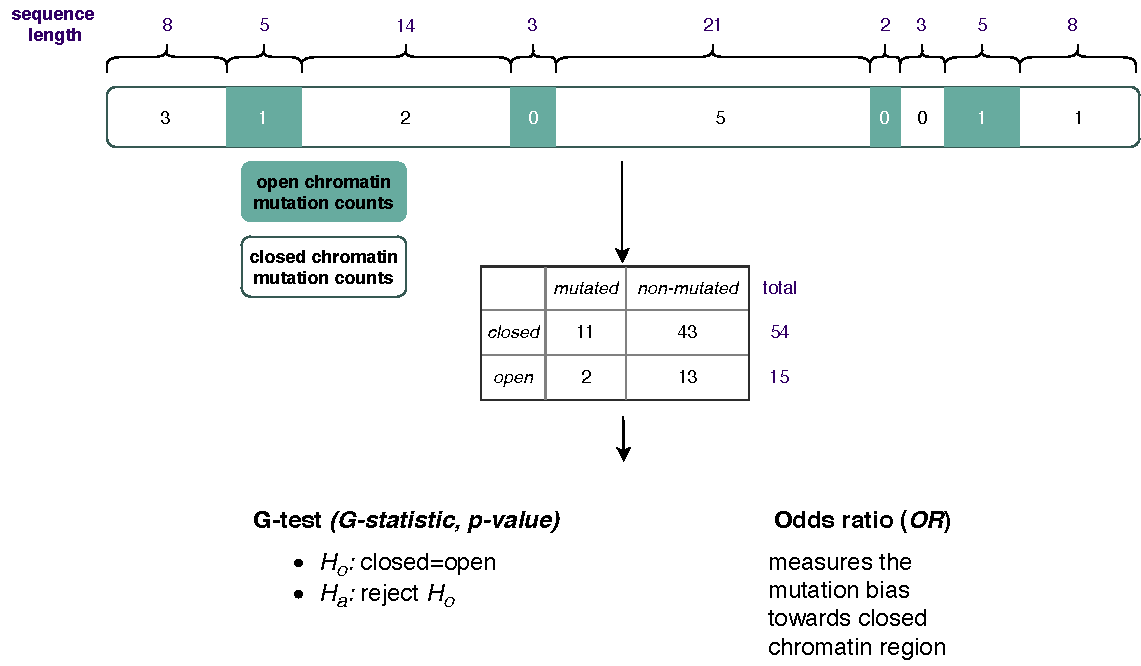
\includegraphics[scale=0.82]{graphics/mutdistribution.pdf}
\caption{}
    % \caption{\textbf{Establishing the relationship between cancer mutation and chromatin structure of the original cell type.} Mutations were sorted into open and closed regions to make a contingency table, from which a G-test can be performed and an Odds-ratio ($OR$) statistic can be calculated. The G-test establishes whether there is a significant bias in mutation location; $OR$ measures the degree of bias towards closed chromatin regions.}
    \label{fig:gle_workflow}
\end{figure}


\subsubsection{Homogeneity test for mutation location between closed and open regions}
I used the G-test of independence \citep{McDonald2014GtestStatistics} to examine the hypothesis whether the distribution of mutations are random across the genome. More formally:

\begin{itemize}
    \item $H_o (Null)$: Mutation abundance is independent of the chromatin status
    \item $H_a (Alternate)$: Mutation abundance is biased by the chromatin status
\end{itemize}

First, the expected number of observations for each cell assuming the null was true was calculated as per Table \ref{tab:count_exp_demo}. For example, the expected number of mutated bases in the closed regions $e_i$ is proportional to the number of bases available in the closed regions $c$ and the number of mutations $m$. The departure of the observed count $o_i$ from the expected $e_i$ was measured by the $G$ statistic, calculated as:
\begin{equation}
    G = 2 \underset{i}{\sum} o_{i} \ln \frac{o_{i}}{e_{i}}
    \label{eq:g}
\end{equation}
where $o_{i}$ are the observed values (\textit{i.e.} entries from Table \ref{tab:count_obs_demo}) and $e_{i}$ are the expected values (\textit{i.e.} entries from Table \ref{tab:count_obs_demo}) and the p-values were obtained by contrasting $G$ against the $\chi^2_1$ distribution. I used Bonferroni method on the p-values for multiple test correction as per equation \ref{eq:bonferroni} in the Appendix \citep{Armstrong2014WhenCorrection}.

\vspace{0.2cm}
\begin{table}[ht!]
\caption{}
    % \caption{Demo contingency tables. Panel (a) contains the observed counts, each of the entries $c_m$, $c_n$, $o_m$ and $o_n$ represents an $o_i$ in equation \ref{eq:g}. Panel (b) contains the expected counts, each of the elements represents an $e_i$ in equation \ref{eq:g}.}
    \begin{subtable}[!h]{.5\textwidth}
        \centering
        \begin{tabular}{r|rr|r}
             & Mutated & Non-mutated & Total  \\
        \hline
            Closed & $c_m$ & $c_n$ & $c$ \\
            Open & $o_m$ & $o_n$ & $o$ \\
        \hline    
             & $m$ & $n$ & $t$ \\
        \end{tabular}
        \vspace{0.2cm}
    \subcaption{Observed counts}
    \label{tab:count_obs_demo}
    \end{subtable} 
    \quad % for side by side tables
    \begin{subtable}[!h]{.5\textwidth}
        \centering
        \begin{tabular}{r|rr|r}
             & Mutated & Non-mutated & Total  \\
        \hline     
            Closed & $c*m/t$ & $c*n/t$ & $c$ \\
            Open & $o*m/t$ & $o*n/t$ & $o$ \\
        \hline    
             & $m$ & $n$ & $t$ \\
        \end{tabular}
        \vspace{0.2cm}
    \subcaption{Expected counts}
    \label{tab:count_exp_demo}
    \end{subtable}    
\end{table}

\subsubsection{Odds ratio for the bias in GLE}
To complement the G-test, I used the odds ratio \citep[$OR$;][]{Hoppe2017OddsRatios} as a measure of preference for mutations to occur in closed chromatin regions compared to open regions. The formula for $OR$ of the contingency Table \ref{tab:count_obs_demo} is as follows:

\begin{equation}
    OR = \frac{c_m/c_n}{o_m/o_n}
    \label{eq:or}
\end{equation}

where $c_m$, $c_n$, $o_m$ and $o_n$ are all observed values that comes from Table \ref{tab:count_obs_demo}.

\subsubsection{Jackknife for the variation of $OR$}
It is worth noting that even within one cancer type, different donors might vary in the number of mutations they carry and the locations of the mutations (\textit{e.g.} if they are an outlier). If a donor has a very distinctive mutation pattern, their data might bias the $OR$ statistic for their whole cancer cohort, especially when the cohort is small. To address this, I performed a jackknife analysis on this measure for each disease \citep{Miller1974TheReview}. An illustration of the jackknife workflow is shown in figure \ref{fig:jackknife_demo}. Specifically, to see how influential a donor $i$ is on $OR$, I removed that donor, recomputed $OR_i$ and computed a pseudo-value for $OR$ as per equation \ref{eq:jackknife}. 

\begin{equation}
    OR^{pseudo}_i = nOR - (n-1)OR_i
    \label{eq:jackknife}
\end{equation}
where $OR^{pseudo}_i$ is the jackknifed pseudo-value for donor $i$, $OR_i$ is the recomputed $OR$ without donor $i$, $n$ is the number of donors.

Applying this to every donor generates a new set of $OR$ that reflects the potential range of the true $OR$. The result for this is shown in Subsection \ref{gle:or}.

\begin{figure}[h!]
    \centering
    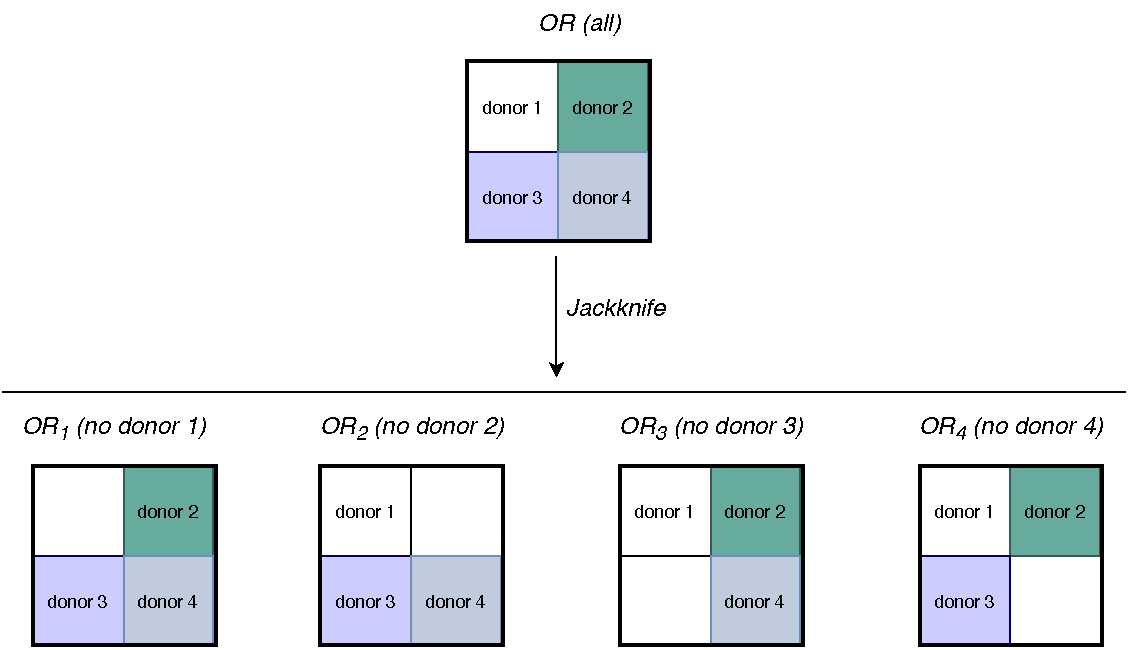
\includegraphics[scale=0.8]{graphics/jackknife_demo.pdf}
\caption{}
    % \caption{\textbf{Illustration of jackknife analysis}. For a hypothetical cancer with 4 donors, the original odds ratio $OR$ was computed. Donor 1 was then omitted and a new odds ratio $OR_1$ was recomputed and a pseudo value $OR^{pseudo}_1$ was obtained. The same was applied to every other donor. The end result was a set of odds ratio statistics $\{OR_1^{pseudo}, \ldots, OR_4^{pseudo}\}$ that were used to estimate the possible range of the true $OR$ statistic}
    \label{fig:jackknife_demo}
\end{figure}


\subsubsection{Mislabelling DHS data}
It is a very natural concern that the calculation of $OR$ is itself biased towards closed chromatin regions purely due to its large size compared to open regions. Besides, if chromatin status is a determinant of mutation location, then cells that have similar DHS should have somewhat similar GLE patterns. To address both of these, I considered all possible combinations of DHS data for the original cell types and mutation data for cancers. Next, instead of calculating $OR$ for the matching DHS/mutation data, I calculated all mislabelled $OR$'s. Eventually, for each cancer, 11 mislabelled $OR$'s and one correctly matched $OR$ were obtained. The result for this is presented in Subsection \ref{gle:mixed_or}.

\subsection{Hypothesis testing of GLE between cancer pairs by bootstrap}\label{methods:bootstrap}

I examined whether GLE could discriminate cancers and what approaches to represent GLE could yield the most resolution. This includes the conventional bin \textit{v.s.} smooth representation and the Wasserstein \textit{v.s.} Euclidean distance measures. 

\subsubsection{Bin \textit{v.s.} smooth representation}
\paragraph{Bin} As briefly described in Figure \ref{fig:mutdistribution_demo}, the bin representation segmented the genome into non-overlapping bins of 1 million bases in length. The number of mutations in each bin was recorded for each chromosome, then divided by the total mutations in that chromosome to get the bin density. 
\paragraph{Smooth} To address the issue with arbitrary boundaries introduced by the discrete bins approach, I proposed a smoothing representation that computes a sliding window of mutation density across each chromosome (Figure \ref{fig:mutdistribution_demo}). This was done using a kernel function \citep[equation \ref{eq:density};][]{Silverman1986DensityAnalysis}. The idea is that the density at a certain location $x$ should be proportional to the distance from $x$ to all other locations $X_i$ where mutations are observed. The closer $x$ is to the observed data $X_i$, the higher the mutation density at $x$.

\begin{equation}
    \hat{f}(x) = \frac{1}{nh} \underset{i=1}{\overset{n}{\sum}} K\Big(\frac{x- X_i}{h}\Big)
    \label{eq:density}
\end{equation}

where $\hat{f}$ is the density for location $x$, $n$ is the total number of mutations, $X_i$'s are all genomic locations where mutations occur, $K$ is the kernel function - here the Gaussian kernel was used (appendix equation \ref{eq:gaussian}), $h>0$ is the bandwidth and determines the level of smoothing to be done. Scott's rule \citep[appendix equation \ref{eq:bandwidth};][]{Scott1992MultivariateEstimation} was used to determine the bandwidth. This was done using the python class \texttt{gaussian\_kde} from \texttt{scipy.stats} \citep{2020SciPy-NMeth}.

\subsubsection{Euclidean \textit{v.s.} Wasserstein distance measure}
I separately used the Euclidean \citep{ONeill2006FrameFields} and Wasserstein \citep{Kolouri2017OptimalApplications} distances for both the bin and the smooth representations to compare the GLE from two cancers. The basic difference between two is depicted in Figure \ref{fig:wasserstein_demo}. In a simple sense, Euclidean measures the distance between two densities in a point-wise manner and in the vertical direction while Wasserstein uses both the vertical and horizontal directions. 

\begin{figure}[h!]
    \centering
    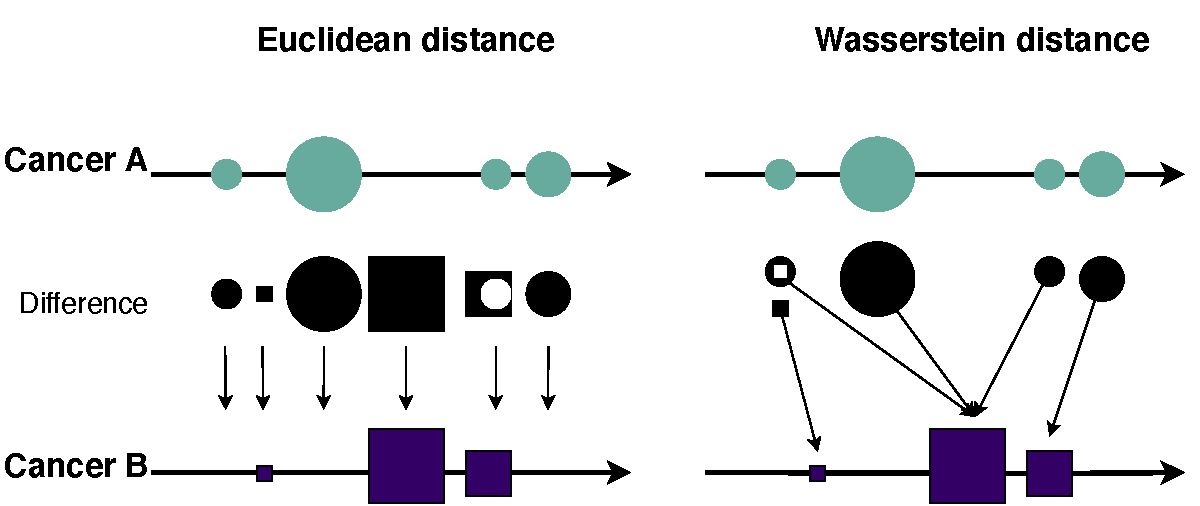
\includegraphics[scale=0.8]{graphics/wasserstein_demo.pdf}
    \caption{\textbf{Schematic diagram for Euclidean and Wasserstein distance between two vectors.} The green circles are data points on the GLE vector for Cancer A, the purple squares are data points on the GLE vector for Cancer B. The black shapes and the arrows combined represent the difference between Cancers A and B. Euclidean is the point-wise difference between the same location on vectors A and B, and is strictly in the vertical direction. In other words, the Euclidean distance between A and B only depends on how different points of similar coordinates are. Wasserstein takes into account both the vertical and horizontal directions; it is intuitively the minimal amount of work required to transport mass from A to B. The Wasserstein distance between A and B depends on both the difference between the magnitude of data points and the path it takes to move data points from A to B.}
    \label{fig:wasserstein_demo}
\end{figure}


\paragraph{Euclidean} The Euclidean distance is also known as the Pythagorean distance. The squared Euclidean distance is the sum of squares of the differences between the two corresponding coordinates of each vector \citep[equation \ref{eq:euclid};][]{ONeill2006FrameFields}.

\begin{equation}
    d_E(a,b) = \sqrt{\sum_{i=1}^n (a_i - b_i)^2}
    \label{eq:euclid}
\end{equation}

where $d_E(a,b)$ is the distance between two vectors $a$ and $b$ that represent the densities of Cancers A and B; $a_i$ and $b_i$ are the $i^{th}$ elements of $a$ and $b$, respectively. This was executed by the python function \texttt{scipy.spatial.distance.euclidean}.

\paragraph{Wasserstein} It is reasonable to view mutation densities as masses of data spatially distributed across a 1-D axis (Figure \ref{fig:wasserstein_demo}). From this viewpoint, Wasserstein appears a well suited measure of distance between two densities. Intuitively, it measures the minimal amount of work required to move mass from Cancer A to B. Mathematically, it does so by searching for the minimum distance with respect to all the joint distributions $\gamma(x,y)$ of random variables $(X,Y)$ that have \glspl{marginal} $a$ and $b$, as follows.

\begin{equation}
    d_W(a,b) = \underset{\gamma \in \mathcal{J}(a,b)}{\inf} \int |x-y| d \gamma(x,y) 
    \label{eq:wassertein}
\end{equation}

where $d_W$ is the Wasserstein distance; $a$ and $b$ are the vectors that represent the densities of Cancers A and B, respectively; $\mathcal{J}$ is the set of all joint distributions $\gamma$. (There are infinite number of joint distributions $\gamma$). The $\gamma(x,y)$ terms represent the transport plans to move data from A to B and the $|x-y|$ term measures the distance to move from A to B to execute that transport plan. The smallest value that takes into account the two terms (selected by the infimum operator $\inf$) is the Wasserstein distance. The Wasserstein distance assumes that A and B have the same masses, which was satisfied because by definition, the area under the curve for densities is always 1. This was done using the python function \texttt{scipy.stats.wasserstein\_distance}.


\subsubsection{The bootstrap}

Having established the representations and distance measures, the next questions are whether the distance is significantly large enough to conclude that the cancer types have different patterns of GLE, and which representation can extract the most information for doing so. For this, I used the bootstrap method \citep{Singh2010BootstrapMethod}, which is based on random re-sampling. For a pair of cancers A and B, the formal hypotheses are

\begin{itemize}
    \item $H_o (Null)$ GLE for A is the same as B
    \item $H_a (Alternate)$ GLE for A is different from B
\end{itemize}

The bootstrap procedure is illustrated in Figure \ref{fig:bootstrap_demo}. For a pair of cancer types A and B with distance $d$, I first aggregated all mutations from the two cancers to create a pool of mutations. I then simulated 2 imaginary cancers 1 and 2 by randomly drawing mutations from that previously constructed mutation pool. The constraint on the simulation was that the total number of mutations in Cancer 1 had to be the same as either A or B - likewise for Cancer 2. This constraint was so that the simulated cancers are as close to the original as possible. I then measured the simulated distance $d_i$ between 1 and 2. This process was repeated 1000 times. To conclude that A and B are significantly different from each other, $d_{obs}$ should be larger than most of the simulated $d_i$. In the end, the number of the simulated distances that are greater than the observed distance between A and B, divided by 1000 was the estimated p-value the hypothesis test. The result for bootstrap hypothesis testing is presented in Section \ref{gle:bootstrap} of Chapter \ref{gle}.

\begin{figure}[h!]
    \centering
    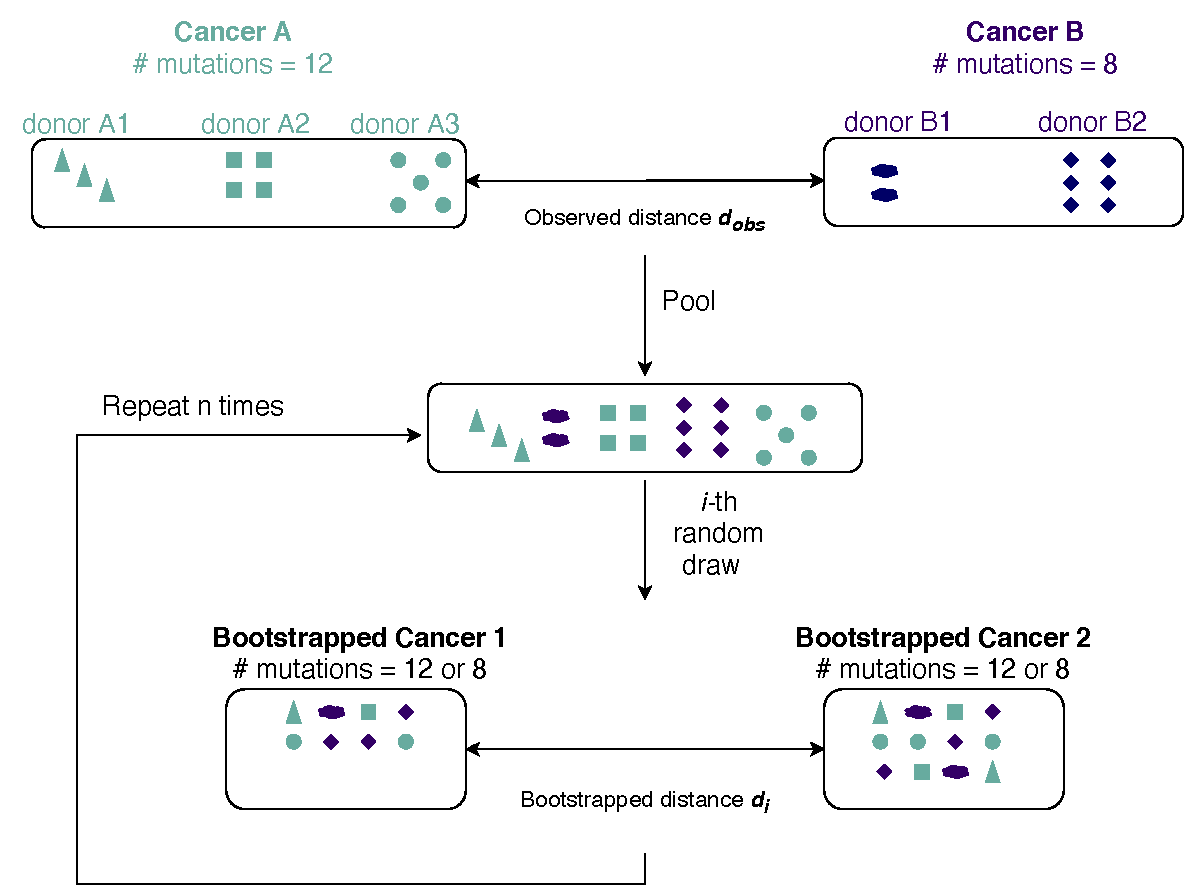
\includegraphics[scale=0.6]{graphics/bootstrap_demo.pdf}
    \caption{\textbf{Testing the hypothesis that two cancers share the same genomic distribution of mutations using bootstrap.} Mutations are pooled from 2 original cancers A and B, the distance between A and B is $d_{obs}$. 2 bootstrapped cancers 1 and 2 are then simulated by randomly drawing mutations from the pool, the number of mutations in 1 and 2 must be the same as either A or B. The distance $d_i$ between cancers 1 and 2 is then measured. This process is repeated 1000 times for each of the representations introduced. The estimated p-value is the number of times $d_i > d_{obs}$ divided by $n$.}
    \label{fig:bootstrap_demo}
\end{figure}


\section{Whole disease analysis of SCE}\label{methods:sce}
Cancers are known to have distinctive compositions of mutations, which themselves consist of two components: the base substitution and the flanking bases. Together, the two components are called sequence context effect (SCE). This section describes the statistical techniques  to measure the information content available in both components.

\subsection{Overview of the techniques to measure information}
The nature of SCE for both the base substitutions and the flanking bases is simply count data determined by categorical variables, which can be displayed on a contingency table. It is straightforward to assign this type of data to have a multinomial distribution. To establish whether or not one categorical variable (\textit{e.g.} the cancers) is deterministic of another (\textit{e.g.} the types of mutations), we can assume product multinomial sampling. Due to the mathematical connection between the product multinomial and Poisson distributions, one could execute this  via a generalised linear model (GLM) under the Poisson distribution \citep{Nelder1974LOGSQUARES.}. This project used the MutationMotif package previously developed in the Huttley lab, whose key function is \texttt{glm} from R \citep{Zhu2017}.

\subsubsection{Generalised linear model}
Table \ref{tab:glm_demo} illustrates how GLM can be used to evaluate whether one categorical variable is associated with another. Specifically, the example tests whether the composition of base substitutions from the wildtype \textbf{T} differs for cancer A and B. Answering this question requires a null model ($H_o$) that assumes no relationship and a saturated model ($H_a$) that assumes an association between cancer types ($\lambda_{cancer}$) and the substitution types ($\lambda_{sub}$). This association manifests through the $\lambda_{cancer:sub}$ that is present in $H_a$ but absent in $H_o$. By measuring the deviance statistic $D$ (equation \ref{eq:deviance}), \textit{i.e.} how much information the null is missing from the saturated model, and contrasting $D$ against the $\chi^2$ distribution, a p-value can be obtained. A small enough p-value (usually $<0.05$) is taken to imply that $\lambda_{cancer}$ is predictive of $\lambda_{sub}$.

\begin{equation}
D = -2 \ln \frac{\hat{L}(saturated)}{\hat{L}(null)}
\label{eq:deviance}
\end{equation}
where $D$ is the deviance statistic; $\hat{L}$ is the estimated maximum likelihood for the parameters in the corresponding models.

\begin{figure}[h!]
  \begin{minipage}[c]{0.5\textwidth}
    \captionof{table}{\textbf{Example of how GLM and RE can be used for categorical data in a contingency table}. In this example, the categorical variable for cancer type $\lambda_{cancer}$ takes values cancer A or cancer B; the variable for the composition of base substitution $\lambda_{sub}$ takes values T$\rightarrow$A, T$\rightarrow$C and T$\rightarrow$G. To establish whether $\lambda_{cancer}$ is explanatory of $\lambda_{sub}$, one can perform a hypothesis test based on a null and a saturated model (formulae \ref{eq:spectra_demo}; the $counts$ corresponds to the $count$ term in equation \ref{eq:spectra_demo}). The hypothesis test outputs a p-value; if p-value is small enough, it can the explanatory relationship. The test also allows estimating $RE$, which measures how much information is contributed by each entry in the table.} 
    \label{tab:glm_demo}
  \end{minipage}\hfill
  \begin{minipage}[c]{0.48\textwidth}
    \begin{tabulary}{\columnwidth}{rRRR}
    \toprule
        & \textbf{T$\rightarrow$A} & \textbf{T$\rightarrow$C} & \textbf{T$\rightarrow$G}  \\
    \hline
        \textbf{Cancer A} & $count_{T>A}$ & $count_{T>C}$ & $count_{T>G}$  \\
        \textbf{Cancer B} & $count_{T>A}$ & $count_{T>C}$ & $count_{T>G}$  \\
    \bottomrule
    \end{tabulary}
    \vspace{1cm}
    \begin{equation}
        \begin{aligned}
            H_o: \ln{count} =& \lambda_{cancer} + \lambda_{sub}  & \\
            H_a: \ln{count} =& \lambda_{cancer} + \lambda_{sub} + \lambda_{cancer:sub}
        \end{aligned}
        \label{eq:spectra_demo}
    \end{equation}
  \end{minipage}
\end{figure}


\subsubsection{Relative entropy}\label{methods:re}
To measure the amount of information contributed by each entry in the contingency table ($count$ in Table \ref{tab:glm_demo}), I used relative entropy ($RE$). $RE_i$ for the entry $i$ can be calculated via the deviance residual $r_i$ of the entry \citep[$r_i$ obtained using appendix equation \ref{eq:dev_res};][]{Zhu2017}, as follows

\begin{equation}
    RE_i = \frac{r_i}{2n} 
    \label{eq:re}
\end{equation}
where $RE_i$ is the relative entropy for entry $i$ of the contingency table; $r_i$ is its deviance residual and $n$ is the total counts. 

Note that while the deviance $D$ measures the departure of the null from the saturated, $r_i$ is the contribution from entry $i$ to this departure, and the sum of all $r_i^2$ is equal to $D$. I chose $RE$ to be the measure of information because it scales the deviance residuals by its sample size, thereby making comparison across hypothesis tests with different amount of data valid. 

\subsection{Base substitutions}\label{methods:spectra}
\subsubsection{Composition of base substitutions for individual cancers}
To examine the patterns of base substitution in a cancer, I calculated the $RE$'s when comparing that cancer to a ``null cancer'', where all mutation counts are the same (Table \ref{tab:glm_spectra}). Due to the difference in the abundance of nucleotides (\textit{e.g.} only about 41\% of the human genome is C+G, the rest is A+T), I separately calculated four $RE$ sets for substitutions that involved different wildtype bases. Table \ref{tab:glm_spectra} illustrates the set whose wildtype base is T. The results for this are available in Subsection \ref{sce:spectra}.

\vspace{0.2cm}
\begin{figure}[h!]
  \begin{minipage}[c]{0.4\textwidth}
    \captionof{table}{\textbf{Contingency table to examine the composition of base substitutions in Cancer A}. Cancer A is compared to a null cancer where all counts are the same. The resulting $RE$'s represent the excess/deficit of certain substitutions. This particular table computes the $RE$ set for substitutions whose wildtype is T. $\lambda_{cancer}$ is a categorical variable taking values \textbf{Cancer A} or \textbf{Null}. $\lambda_{sub}$ indicates whether the counted substitution is \textbf{T$\rightarrow$A}, \textbf{T$\rightarrow$C} or \textbf{T$\rightarrow$G}. For each cancer, three similar tables are required for substitutions of A, C and G.} 
    \label{tab:glm_spectra}
  \end{minipage}\hfill
  \begin{minipage}[c]{0.59\textwidth}
    \begin{tabulary}{\columnwidth}{lCCCR}
    \toprule
        & \textbf{T$\rightarrow$A} & \textbf{T$\rightarrow$C} & \textbf{T$\rightarrow$G}  & \textbf{total} \\
    \hline
        \textbf{Cancer A} & $count_{T>A}$ & $count_{T>C}$ & $count_{T>G}$ & $count_{tot}$ \\
        \textbf{Null} & $count_{tot}/3$ & $count_{tot}/3$ & $count_{tot}/3$ & $count_{tot}$ \\
    \bottomrule
    \end{tabulary}
    \vspace{0.9cm}
    \begin{equation}
        \begin{aligned}
            H_o: \ln{count} =& \lambda_{cancer} + \lambda_{sub}  & \\
            H_a: \ln{count} =& \lambda_{cancer} + \lambda_{sub} + \lambda_{cancer:sub}
        \end{aligned}
        \label{eq:spectra}
    \end{equation}
  \end{minipage}
\end{figure}


\subsubsection{Base substitutions across cancers}
Having looked at the base substitutions for individual cancers, I examined how well base substitutions can be used to discriminate cancers. To compare two cancers, the contingency table for this analysis is similar to the example in Table \ref{tab:glm_demo}. Similar to the case of individual cancers, I analysed mutations from different wildtype bases separately using the so-called mutation spectrum test of \citet{Zhu2017}. In addition to the $RE$'s, also looked at the p-values from the hypothesis tests. Since there are four hypothesis tests, there are four p-values, which I combined these p-values into one p-value using the Fisher's method \citep[details in \ref{apdx:fisher};][]{Fisher1992StatisticalWorkers}. Briefly, Fisher's method adds up all the logs of the member p-values, this value is doubled and contrasted against the $\chi^2$ distribution to obtain the final joint p-value. 66 joint p-values were obtained and adjusted using Bonferroni multiple test correction \citep[equation \ref{eq:bonferroni};][]{Armstrong2014WhenCorrection}.

\subsection{Flanking bases}\label{methods:nbr}
In this subsection, we are interested in the information content available in the flank base component of SCE, including positions -1, +1, -2 and +2 with respect to the mutation. This is the neighbour analysis from \citet{Zhu2017}. As for the base substitution analyses, I separated the analysis for different mutations due to their different frequencies of occurrence. Figure \ref{fig:nbr_demo} illustrates how information can be measured for position +1 of the C$\rightarrow$T mutation in some cancer A. Specifically, the analysis measures the extent to which bases found next to the C$\rightarrow$T mutation tend to differ from bases next to a randomly selected C in the genome. To do this, for each C$\rightarrow$T substitution, a random C within the neighbourhood of 500 bases to each side of the substitution was selected and its flanking base at position +1 was recorded. I then received a contingency table. Using the models in formulae \ref{eq:nbr_demo}, I obtained the $RE$'s, as described in subsection \ref{methods:re}, whose total is the desired measure of information. I measured the total $RE$ for all other flank positions of the 5-mer context and all other mutations.

\begin{figure}[h!]
  \begin{minipage}[c]{0.48\textwidth}
    \caption{
      \textbf{The smoothing approach is expected to be more robust than the bin approach.} Both panels depict the same mutation location data for a hypothetical chromosome, with the black dots below the x-axis representing the true location of mutations. By binning the genome by convention, one counts the number of mutations in each green bin. The obtained GLE data is then the green dots on top of each bin. This binned GLE data changes when shifting the bin boundaries from panel (a) to panel (b). On the contrary, the smooth representation of GLE, which adopts \gls{density} estimation, is depicted by the purple dots on the purple line. By smoothing the genome, GLE data is the same for both panels. 
    } \label{fig:mutdistribution_demo}
  \end{minipage}\hfill
  \begin{minipage}[c]{0.55\textwidth}
    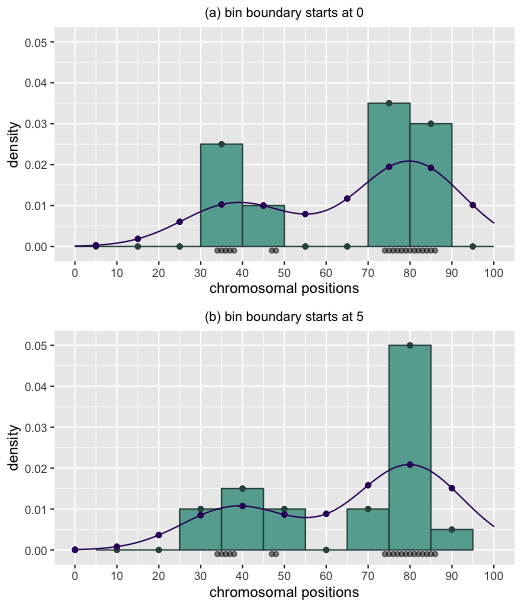
\includegraphics[width=\textwidth]{graphics/mutdistribution_demo.png}
  \end{minipage}
\end{figure}


\section{Mutation-based classifier for cancers}\label{methods:ml}
Based on the premise that GLE and SCE are important aspects of a cancer mutation profile, this section explores how we could exploit the information from GLE and SCE for cancer classification. Because I trialled different approaches to represent data, I expect the known properties of the best performing approach should reveal important characteristics of the data. More critically, it should validate the findings from whole disease analyses, thereby consolidating our understanding of cancer mutagenesis.

\subsection{Machine learning workflow}\label{methods:ml_workflow}
For all classifiers trained in the subsequent subsections, I followed the same training procedures \citep{Zengyou2015DataApplications}. 

\subsubsection{$K$-nearest neighbours}
One algorithm that uses pairwise distances between observations to describe both GLE and SCE is the $K$-nearest neighbours \citep[KNN;][]{Neath2010DiscriminationClassification}. There are two reasons there was a preference for distances over raw feature vectors (\textit{i.e.} the bin/smooth vector of density for GLE or the mutation count vector for SCE). First, as in the case for most biological data, our data suffered from the curse of dimensionality \citep{Banks2003DataStatistics}, meaning there were more parameters than there were observations, making inference less robust. For example, the bin representation for GLE alone has about 3000 parameters corresponding to $\approx$3000 bins, while there are only about hundreds of donors available. Describing data in terms of distances is therefore a way to escape the curse of dimensionality (training $\approx$3000 parameters on a few hundred observations). Second, I was interested in experimenting with different types of metrics that might better describe the data than the typically default Euclidean distance, such as the Wasserstein and Jensen-Shannon distance. The principle of the KNN algorithm is straightforward (Figure \ref{fig:knn_demo}). The input into the classifier is a pairwise distance matrix between all donors. When prediction on an unknown donor needs to be made, KNN calculates the distances from the unknown to all known donors in the training set and identifies the nearest training points (known neighbours) to the unseen donor. The predicted cancer will be the predominant cancer within these neighbours. This was done using \texttt{sklearn.neighbors.KNeighborsClassifier} \citep{scikit-learn}.

\begin{figure}[ht!]
    \centering
    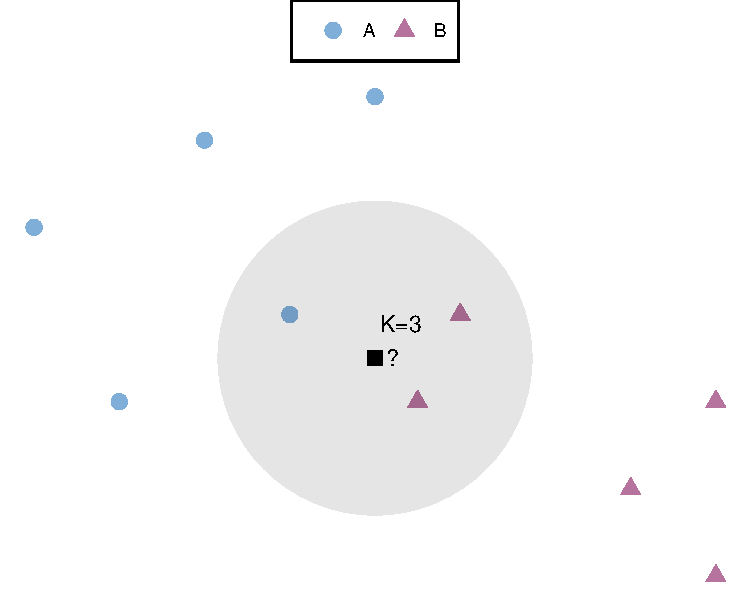
\includegraphics[scale=0.8]{graphics/knn_demo.pdf}
    \caption{\textbf{Illustration of K-nearest neighbours (KNN) algorithm.} When K=3, 3 neighbours to the new donor are identified based on the pre-calculated distances. The 3 neighbours get to ``vote'' for the prediction made on the new donor. Because there are 2 B's and 1 A, the new donor has cancer B.}
    \label{fig:knn_demo}
\end{figure}


\newpage
\subsubsection{F1-score}
I used F1-score to measure the accuracy of the models in the validation step \citep{Kulkarni2020FoundationsDemocracy}. $F1$ is a typically recommended measure of accuracy as it is the combination of sensitivity and specificity of the predictions (equation \ref{eq:f1}). Taking Cancer A as an example, sensitivity refers to how well a model can recognise Cancer A (equation \ref{eq:sensitivity}), and specificity refers to how likely a sample is Cancer A if it is predicted to be Cancer A (equation \ref{eq:specificity}). To get the overall $F1$ for the model, I calculated $F1$ for each cancer and averaged them, weighing by the true instances in each cancer.

\begin{equation}
    F1 = 2\frac{sensitivity \times specificity}{sensitivity + specificity}    
    \label{eq:f1}
\end{equation}

\subsubsection{Cross validation}
Training a KNN classifier where inputs are distances, as in our case, simply means choosing the number of neighbours $K$ used for prediction. This process is also called hyper-parameter tuning, illustrated in Figure \ref{fig:cv_demo}. Specifically, I saved 1/10 of the data to be the test set. I then split the remaining training set (9/10 of the data) into five folds (or sections). Note that the proportions of different cancers were the same for all splits. The first four folds were visible to the model and are called the training set; meanwhile, the 5$^{th}$ fold was not seen by the model and is called the validation set. The ``$K$'' in KNN represents the number of neighbouring observations used for prediction. I trialled $K$ from 1 to $n$, where $n$ was the number of donors available in the cancers with fewest donors in the validation set. By contrasting the prediction made by the test set against the validation set, each trial outputs an $F1$. I then repeated the 5-fold cross validation procedure by sequentially replacing the 5$^{th}$ fold with the other folds. Eventually, I was able to pick the $K$ with the highest average $F1$. I then applied this $K$ to the test set to obtain the final $F1$. The whole process was repeated 10 times to establish a sense of variation in the final accuracy evaluation.

\begin{figure}[h!]
    \centering
    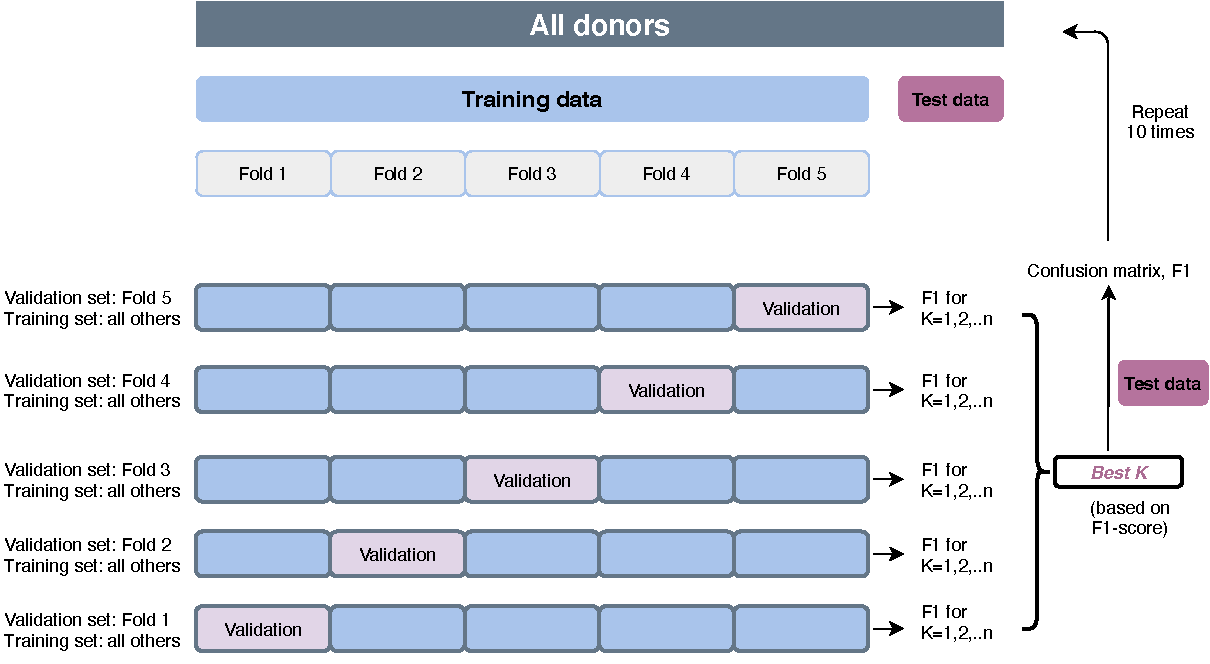
\includegraphics[scale=0.78]{graphics/ML_demo.pdf}
    \caption{\textbf{Illustration of machine learning cross validation workflow.} Data was split into a test set (1/10) and a training set (9/10). The training set was divided into 5 folds, each fold was sequentially used as a validation set to select the parameter $K$ of the model. From the set of $F1$'s for each $K$, I selected the best $K$. This $K$ was then applied to the test set for final evaluation (1/10 of the data). The whole process was repeated 10 times to evaluate the possible range of the accuracy, reported in the form of confusion matrices or $F1$.}
    \label{fig:cv_demo}
\end{figure}


\subsection{Classifier by GLE}
To classify cancers based on GLE, I experimented with two representations: bin \& smoothing and two distance measures: Euclidean \& Wasserstein distance. Details about the techniques of these representations and measures have been described in subsection \ref{methods:bootstrap}. The difference is that this section is on the individual donor scale. Briefly, for each donor, GLE was represented in the form of either the bin or the smoothing approach. For each representation, Euclidean or Wasserstein distances were then calculated for each pair of donors. The classifier was then trained as per the procedure outlined above. The results for this are available in Section \ref{ml:gle} of Chapter \ref{ml}.

\subsection{Classifier by SCE}\label{methods:ml_sce}
In this subsection, I trialled different representations of SCE, all representations used the Jensen-Shannon distance. 

\subsubsection{Jensen-Shannon distance}
I used Jensen-Shannon distance \citep[JSD;][]{Osterreicher2003} as the measure of distance to classify cancers based on SCE. JSD is an appropriate measure for composition data like SCE because it gives weights to the more dominant elements. For example, the contribution of C$\rightarrow$T mutations to the JSD between two donors depends on both the difference in  C$\rightarrow$T and the abundance of C$\rightarrow$T in the two donors. Additionally, JSD is the symmetric version of the Kullback-Leibler divergence \citep{Kullback1951}. It is calculated as follows:

\begin{equation}
    d_{JS}(P,Q) = \sqrt{\frac{1}{2} (d_{KL}(P|M) + d_{KL}(Q|M))}
\end{equation}
where $d_{JS}(P,Q)$ is the JSD between the SCE of donors P and Q; M is the average between P and Q: $M = \frac{P+Q}{2}$; $d_{KL}(P|M)$ is the Kullback-Leibler divergence of M from P, likewise for Q. $d_{KL}$ can be calculated as per equation \ref{eq:kl} in the appendix.

The representations of the vectors to train the KNN classifier based on JSD are described below.

\subsubsection{Comparing 1-mer, 3-mer and 5-mer}
Due to SCE's nature as composition data, one obvious way to represent SCE is the proportion of mutations. To be precise, the vector that represents SCE for a donor is the count of different mutation types, divided by the total number of mutations. The generation of the count vector is illustrated in Figure \ref{fig:get_sce}. However, it is worth noting that as the k-mer size increases, the number of elements in the SCE vector increases very rapidly, according to equation \ref{eq:sce_counts} (Figure \ref{fig:sce_size}).

\begin{figure}[ht!]
    \begin{subfigure}{\textwidth}
    \centering
    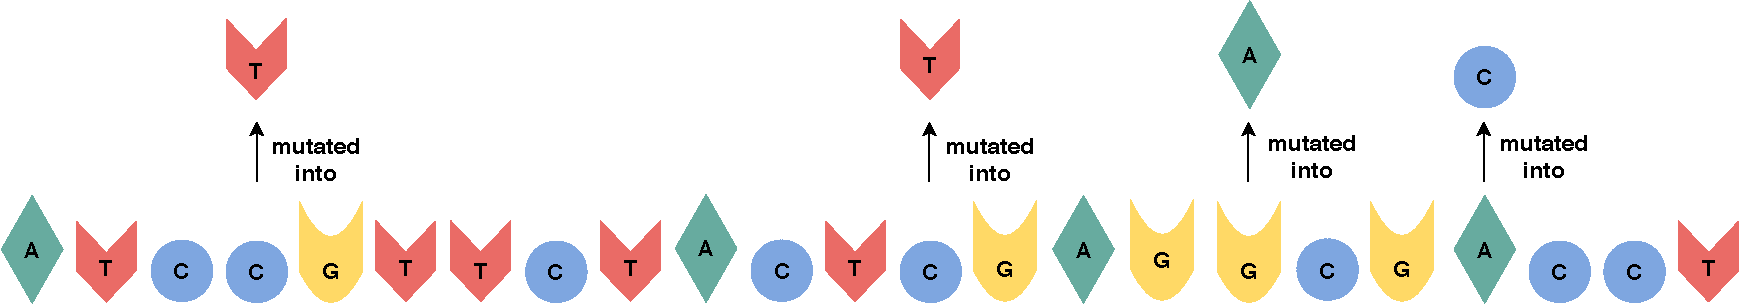
\includegraphics[scale=0.5]{graphics/sce_counts.pdf} \\
    \vspace{0.9cm}
    \begin{tabulary}{\columnwidth}{cc|cc|cc}
    \toprule
        \multicolumn{2}{c}{\textbf{1-mer}}  & \multicolumn{2}{c}{\textbf{3-mer}} & \multicolumn{2}{c}{\textbf{5-mer}} \\
        \hline
        mutation & count vector & mutation & count vector & mutation & count vector \\
    \hline
        [A$\rightarrow$C] & 1 & G[A$\rightarrow$C]C & 1 & CG[A$\rightarrow$C]CC & 1 \\
        
        [C$\rightarrow$T] & 2 & C[C$\rightarrow$T]G & 1 & TC[C$\rightarrow$T]GT & 1 \\
        
         &  & T[C$\rightarrow$T]G & 1 & CT[C$\rightarrow$T]GA & 1 \\
         
        [G$\rightarrow$A] & 1 & G[G$\rightarrow$A]C & 1 & AT[G$\rightarrow$A]CG & 1 \\
        
        ... & 0 & ... & 0 & ... & 0 \\
    \bottomrule
    \end{tabulary}
    \caption{Generating the count vector for 1-mer, 3-mer and 5-mer}\label{fig:get_sce}
    \end{subfigure} \\

  \vspace{1cm}
  \begin{subfigure}{\textwidth}
  \begin{minipage}{0.65\textwidth}
    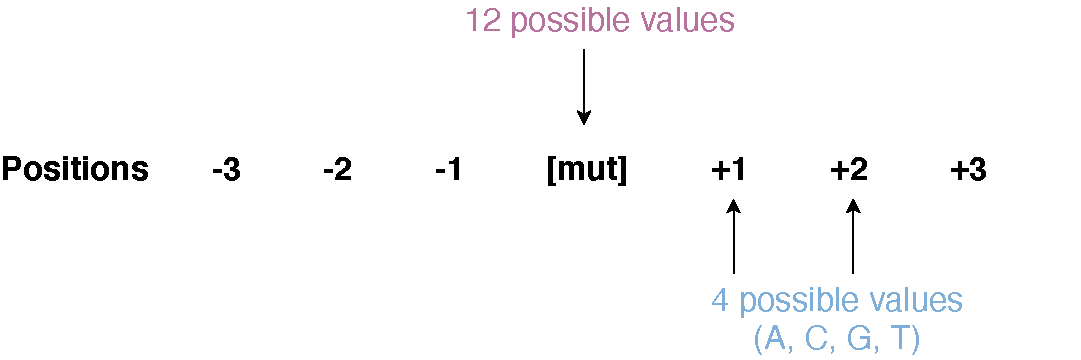
\includegraphics[width=\textwidth]{graphics/sce_counts_demo.pdf}
  \end{minipage}
  \begin{minipage}{0.3\textwidth}
    \begin{equation}
    l = 12 \times 4^{k-1}
    \label{eq:sce_counts}
    \end{equation}
    where $l$ is the number of elements and $k$ is the k-mer size, so $k-1$ is the number of flanking bases involved
  \end{minipage}
    \caption{Total number of elements for SCE incorporating flanking positions}\label{fig:sce_size}
  \end{subfigure} \\
  \vspace{0.2cm}
  \caption{
%   \textbf{The number of elements increases extremely rapidly with increasing k-mer size.} This is because there are 12 possible mutations, and for each flanking position, there are 4 possible bases. Panel (a) gives an example of how the count vector for SCE is generated for 1-mer, 3-mer and 5-mer for a DNA sequence with 4 mutations. The elements in the count vector were then divided by the total number of mutations to obtain the SCE vector. Panel (b) illustrates how to calculate the number of elements given the $k$-mer size. 
} \label{fig:sce_counts}
\end{figure}


\subsubsection{Strand asymmetric, semi-symmetric and fully-symmetric representations}
The rapid growth in the number of mutations when incorporating more flanking positions inevitably results in sparse vectors with many 0 values, as some donors only have hundreds of mutations. Accordingly, I investigated whether introducing strand symmetry, at the expense of some information loss, could address this issue. Therefore, this analysis could also reveal a mechanism of mutagenesis in cancer, which is whether mutation strand symmetry exists or not. There are three levels of strand symmetry involved, asymmetry, semi-symmetry and full-symmetry. Specifically, asymmetry is the normal mutation counts described above. For semi-symmetry, as described in Figure \ref{fig:motif_symmetric_demo}, whatever mutations that start with G or T were counted as part of the mutations on their reverse complementary strand. This is the representation adopted by the common literature such as \citet{Jiao2020}. The fully symmetric representation is even more stringent, it restricts the alphabet of the flanking bases to be A and C rather than A, C, T and G. This means that on the flanking base components, T was counted as A and G was counted as C. Table \ref{tab:sce_symmetric} summarises the properties of the three representations.

\begin{table}[ht!]
\centering
\caption{}
% \caption{\textbf{Summary of the number of elements available in the vectors for three levels of strand symmetry imposed on SCE.} Similarly to equation \ref{eq:sce_counts}, $l$ is the number of elements in the SCE vector, $k$ is the k-mer size}
\label{tab:sce_symmetric}
\begin{tabulary}{\textwidth}{ lrrr }
\toprule
 & \textbf{asymmetry} & \textbf{semi-symmetry} & \textbf{full-symmetry} \\
 $k$(-mer) & $l = 12 \times 4^{k-1}$ & $l = 6 \times 4^{k-1}$ & $l = 6 \times 2^{k-1}$ \\
\hline

1 & 12 & 6 & 6 \\
3 & 192 & 96 & 24 \\
5 & 3072 & 1536 & 96 \\

\bottomrule

\end{tabulary}
\end{table}


\subsubsection{Dissecting the 5-mer sequence context}
A second approach to reduce the sparsity of large sequence contexts (in this case 5-mer), without loss of information, is to dissect them into smaller submotifs. Specifically, instead of one count vector that incorporates all substitutions flanking positions of 5-mer, I computed multiple submotif vectors that incorporate 1 (2-submotif) or 2 (3-submotif) flanking positions with the mutations. A summary of these representations is presented in table \ref{tab:submotif}. While my previous approaches approaches used one single type of vector to generate a single pairwise distance matrix. The approach in this subsection computed pairwise distance matrices for all submotif vectors, and amalgamated these matrices by averaging all their elements. The resulting pairwise distance matrix was used to train the classifier for submotifs. 

\begin{table}[hp!]
\centering
\caption{\textbf{Summary of the properties of the representations that dissect 5-mer into smaller submotifs.} 2-submotif has 4 component vectors; 3-motif has 3 component vectors. \textbf{\#elements} are the number of elements available in each component vector.}
\label{tab:submotif}
\begin{tabulary}{\textwidth}{ lllllL }
\toprule
 & \textbf{vector 1} & \textbf{vector 2} & \textbf{vector 3} & \textbf{vector 4} & \textbf{\#elements} \\
\hline
2-submotif & (mut, pos-2) & (mut, pos-1) & (mut, pos+1) & (mut, pos+2) & 48 \\
3-submotif & (mut, pos-2,-1) & (mut, pos-1,+1) & (mut, pos+1,+2) & & 192 \\
whole-5mer & (mut, all 4 pos) & & & & 3072 \\
\bottomrule
\end{tabulary}
\end{table}


\subsection{Combining GLE with SCE in a joint classifier}\label{methods:ml_both}
Because GLE and SCE are distinct types of information, in this section, I attempted to combine the two factors to see if it could further improve the predictive power compared to each factor by itself.

\subsubsection{Kernel normalisation}
GLE and SCE have different units, leading to the need to normalise them. By normalising the data, the joint classifier can simultaneously avoid one factor being dominated by the other purely due to their mismatched numerical scales and assess which factor was the stronger predictor of cancer type. For each factor, the normalisation step was done while converting its pairwise distance matrix into a pairwise kernel matrix. It is worth noting that intuitively, the distance matrix measures the difference between data points and kernel matrix measures the similarity between them. I used the Laplacian kernel function for each element of the distance matrix \citep{Wang2016ApplicationFunction}, as follows:

\begin{equation}
    k(x,y) = \exp\bigg( - \frac{d(x,y)}{\sigma}\bigg)
    \label{eq:laplacian}
\end{equation}
where $k$ is an entry of the resulting kernel matrix corresponding to the pair of data points (\textit{i.e.} donors) $x$ and $y$; $d(x,y)$ is the distance between $x$ and $y$ in the distance matrix; $\sigma$ is intuitively the scale parameter. I set $\sigma$ as the median of the distance matrix, excluding the case where $x$ and $y$ were the same. The division by $\sigma$ ensured that the distances in the normalised matrices were numerically on the same scale.

After the normalisation step, I obtained a normalised pairwise kernel matrix $G$ for GLE and $S$ for SCE.

\subsubsection{Weighted combination of GLE and SCE}
I trialled different weights on the linear combination of the kernel matrices $G$ and $S$ according to equation \ref{eq:joint}

\begin{equation}
    J = gG + (1-g)S
    \label{eq:joint}
\end{equation}
where $J$ is the joint kernel matrix; $G$ and $S$ are the kernel matrices for GLE and SCE; $g$ is the weight given to $G$, $1-g$ is the weight given to $S$, $g$ and $1-g$ take values 0, 0.1, 0.2,..., 1. I then converted the joint kernel matrix $J$ into a joint distance matrix $D_J$ using the standard generic approach \citep[more in the appendix equation \ref{eq:k2d_ori};][]{Phillips20112Distance}

\begin{equation}
    d_J(x,y) = \sqrt{2 - 2k(x,y)}
    \label{eq:k2d}
\end{equation}
where $d_J(x,y)$ is the entry for $x$ and $y$ to the joint distance matrix $D_J$; $k(x,y)$ is the entry to the joint kernel matrix $J$.

The subsequent training step proceeded as described in subsection \ref{methods:ml_workflow}. Figure \ref{fig:joint} summarises the procedure for training the joint classifier.

\begin{figure}[ht!]
    \centering
    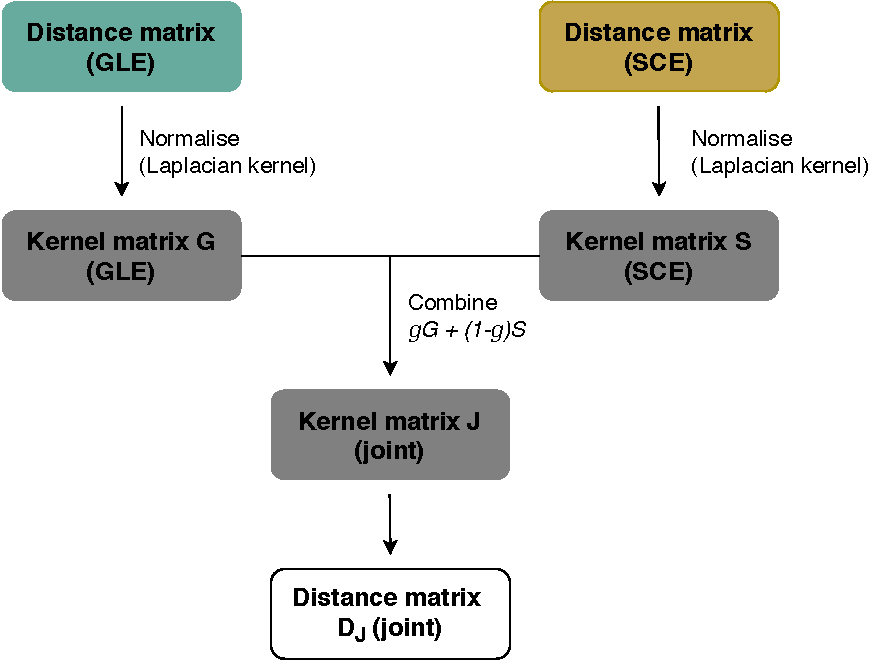
\includegraphics[scale=0.8]{graphics/joint_classifier.pdf}
    \caption{\textbf{Summary of the methods to train the joint classifier for GLE and SCE}. The pairwise distance matrix for each factor was converted to a kernel matrix, normalised and linearly combined with weights $g$ and $1-g$ to get the joint kernel matrix $J$ (equation \ref{eq:joint}). $J$ was then converted back to a distance matrix $D_J$ using equation \ref{eq:k2d}. $D_J$ was subsequently used for model training.}
    \label{fig:joint}
\end{figure}




\bibliographystyle{geneticsstyle}
\bibliography{references,references_extended}
\addcontentsline{toc}{chapter}{Bibliography}

\end{document}
